\documentclass[openany]{book}
\input{notes_white}
\usepackage{mathtools}
\usepackage{pgfplots}
\begin{filecontents*}{temp.dat}
1 1 1
1 2 0.8
1 3 0.5
1 4 0.3
1 5 0.1
2 1 0.8
2 2 1
2 3 0.6
2 4 0.4
2 5 0.2
3 1 0.5
3 2 0.6
3 3 1
3 4 0.7
3 5 0.3
4 1 0.3
4 2 0.4
4 3 0.7
4 4 1
4 5 0.5
5 1 0.1
5 2 0.2
5 3 0.3
5 4 0.5
5 5 1
\end{filecontents*} 
\settitle{Probability and Stats 1  Notes and Solutions}
\begin{document}
\title{\Large{\underemphasise{Probability and Statistics Notes}} \\ \vspace{5pt}
\large{Prob Stats 1: Notes, Exercises and PYQs}}
\author{Eklavya Raman \\ \vspace{5pt} er24ms024@iiserkol.ac.in \\ \vspace{5pt}}
\date{\today}
\maketitle
\tableofcontents
\listoftheorems[
    show=mytheorem,
    title={List of Theorems}]
\part{Probability}
\chapter{Basic Definitions and Concepts}
\section{Sample Spaces and Random Experiments}
\subsection{Definitions}
\begin{mydefinition}{Random Experiment}
A random experiment is a process or action that leads to one or more outcomes that cannot be predicted with certainty. The conditions for a experiment to be classified as a random experiment are: 

\begin{enumerate}
    \item All possible outcomes of the experiment must be known in advance.
    \item The experiment must be repeatable under the same conditions.
    \item The outcome of the experiment must be uncertain, that is we cannot predict its outcome with certainty.
\end{enumerate}
\end{mydefinition}
\begin{example}
    The classic example of a random experiment is the tossing of a fair coin. The possible outcomes are heads or tails, and we cannot predict with certainty which outcome will occur on any given toss. The experiment can be repeated multiple times under the same conditions. 
\end{example}

\begin{example}
    Another example of a random experiment is rolling a fair six-sided die. The possible outcomes are the numbers 1 through 6, and we cannot predict with certainty which number will appear on any given roll. The experiment can be repeated multiple times under the same conditions.
\end{example}

\begin{example}
    A third example of a random experiment is drawing a card from a standard deck of 52 playing cards. The possible outcomes are the 52 individual cards, and we cannot predict with certainty which card will be drawn. The experiment can be repeated multiple times under the same conditions.
\end{example}


\begin{mydefinition}{Sample Space}
The sample space is the set of all possible outcomes of a random experiment. We denote the sample space by the symbol $S$ or $\Omega$.
\end{mydefinition}

\begin{example}
    Consider the random experiment of tossing a fair coin. The sample space for this experiment is $S = \{H, T\}$, where $H$ represents heads and $T$ represents tails.
\end{example}

\begin{example}
    Consider the random experiment of rolling a fair six-sided die. The sample space for this experiment is $S = \{1, 2, 3, 4, 5, 6\}$.
\end{example}

\begin{example}
    Consider the random experiment of drawing a card from a standard deck of 52 playing cards. The sample space for this experiment is $S = \{A\heartsuit, 2\heartsuit, \ldots, K\spadesuit\}$.
\end{example}


\begin{mydefinition}{Event}
    An event is a subset of the sample space. It can consist of one or more outcomes. We denote an event by a capital letter, such as $A$, $B$, or $C$.
\end{mydefinition}

\begin{example}
    Consider the random experiment of rolling a fair six-sided die. The sample space for this experiment is $S = \{1, 2, 3, 4, 5, 6\}$. An example of an event could be $A = \{2, 4, 6\}$, which represents the event of rolling an even number.
\end{example}
\begin{example}
    Consider the random experiment of drawing a card from a standard deck of 52 playing cards. The sample space for this experiment is $S = \{A\heartsuit, 2\heartsuit, \ldots, K\spadesuit\}$. An example of an event could be $B = \{A\heartsuit, 2\heartsuit, 3\heartsuit\}$, which represents the event of drawing a heart with a value of 1, 2, or 3.
\end{example}

\begin{mydefinition}{Exhaustive Sample Space}
A sample space is said to be exhaustive if it includes all possible outcomes of a random experiment.
\end{mydefinition}
\begin{example}
    Consider the random experiment of rolling a fair six-sided die. The sample space for this experiment is $S = \{1, 2, 3, 4, 5, 6\}$. This sample space is exhaustive because it includes all possible outcomes of the experiment.
\end{example}

\begin{mydefinition}{Equilikely Events and Mutually Exclusive Events}
\underemphasise{Equilikely Events:} Two or more events are said to be equilikely if they have the same probability of occurring. For example, when rolling a fair six-sided die, the events of rolling a 1, 2, 3, 4, 5, or 6 are all equilikely because each event has a probability of $\frac{1}{6}$. \\
\underemphasise{Mutually Exclusive Events:} Two or more events are said to be mutually exclusive if they cannot occur at the same time. For example, when rolling a fair six-sided die, the events of rolling a 1 and rolling a 2 are mutually exclusive because both outcomes cannot happen simultaneously. In set theoretic notation, we can define mutually exclusive events as follows: \\
$$A \cap B = \emptyset$$
\end{mydefinition}
We give a few examples of mutually exclusive events and events which are not below: \\
\begin{example}
    Consider the random experiment of rolling a fair six-sided die. The events of rolling a 1 and rolling a 2 are mutually exclusive because both outcomes cannot happen simultaneously.
\end{example}

\begin{example}
Consider the example of events which are not mutually exclusive. Consider the random experiment of drawing a card from a standard deck of 52 playing cards. The events of drawing a heart and drawing a face card are not mutually exclusive because it is possible to draw a card that is both a heart and a face card, such as the King of Hearts.
\end{example}

\section{Probability}
\subsection{Classical Definition of Probability}
\begin{mydefinition}{Classical Probability}
The classical definition of probability states that the probability of an event is the ratio of the number of favorable outcomes to the total number of possible outcomes, provided that all outcomes are equally likely. \\
Let $A$ be an event in the sample space $\Omega$. Let $N$ be the total number of exhaustive, mutually exclusive and equilikely outcomes in $\Omega$. Let $N_A$ be the number of favorable outcomes for the event $A$. Then, the probability of the event $A$, denoted by $P(A)$, is given by:
$$P(A) = \frac{N_A}{N}$$
\end{mydefinition}
\begin{mynote}
The classical definition of probability is applicable in situations where all outcomes are equally likely, such as rolling a fair die or drawing a card from a well-shuffled deck. Furthermore, the classical definition of probability is not applicable in situations where the outcomes are not equally likely, such as in real-world scenarios where certain outcomes may be more probable than others. \\
The classical definition of probability also does not consider infinite sample spaces, where the number of possible outcomes is infinite. In such cases, other definitions of probability, such as the frequentist or Bayesian definitions, may be more appropriate.
\end{mynote}
\begin{example}
    Let us consider the experiment of drawing a card from a standard deck of 52 playing cards. We want to find the probability of drawing an Ace. \\
    By the classical definition, say we repeat the experiment of drawing a card from the deck a large number of times. Let $N$ be the total number of times we draw a card, and let $N_A$ be the number of times we draw an Ace. Then, the probability of drawing an Ace is given by:
    $$P(Ace) = \frac{N_A}{N}$$
    However, we might get different results every time we repeat the experiment if we only follow the classical definition. \\ 
    For example, consider that we first do the experiment and draw cards repeatedly 50 times, out of which we get 5 Aces. Then, the probability of drawing an Ace is given by:
    $$P(Ace) = \frac{5}{50} = \frac{1}{10}$$
    Let's say we repeat the experiment again and this time we draw cards repeatedly 100 times, out of which we get 20 Aces. Then, the probability of drawing an Ace is given by:
    $$P(Ace) = \frac{20}{100} = \frac{1}{5}$$
    This tells us that the classical definition of probability is not very reliable, especially if the number of trials is small.
\end{example}

\subsubsection{Conditions for Classical Definition of Probability}
The classical definition of probability is based on the following conditions:
\begin{itemize}
    \item The sample space must be finite or at most countably infinite.
    \item All outcomes in the sample space must be equally likely.
    \item All events must be exhaustive that is must be subsets of $\Omega$.
\end{itemize}
\begin{mydefinition}{Complement of an Event}
The complement of an event $A$, denoted by $A^C$ or $\overline{A}$, is the event that includes all outcomes in the sample space $\Omega$ that are not in $A$. Formally, it can be defined as:
$$A^C = \Omega \setminus A$$
\end{mydefinition}
\begin{example}
    Consider the random experiment of rolling a fair six-sided die. The sample space for this experiment is $S = \{1, 2, 3, 4, 5, 6\}$. Let $A$ be the event of rolling an even number, that is $A = \{2, 4, 6\}$. The complement of the event $A$, denoted by $A^C$, is the event of rolling an odd number, that is $A^C = \{1, 3, 5\}$.
\end{example}
\subsubsection{Properties of Classical Probability}
We can define the probability function as follows: 
\begin{align*}
P: \Omega \to [0, 1] \\ \sum_{i=1}^{n} P(A_i) = 1
\end{align*}
Therefore, we can write the properties of the probability set function as follows:
\begin{itemize}
\item $0 \leq P(A) \leq 1$ for any event $A$.
\item $\sum_{i=1}^{n} P(A_i) = P(\Omega) =1$ for a exhaustive set of mutually exclusive events.
\item $P(\emptyset) = 0$
\item Impossible event has probability 0, since it has no favorable outcomes.
\end{itemize}
\subsection{Properties of Events and their probabilities}
\begin{mytheorem}[Probability of union - Inclusion Exclusion Formula]
    Let $A$ and $B$ be two events. Then, the probability of the union of $A$ and $B$ is given by:
    $$P(A \cup B) = P(A) + P(B) - P(A \cap B)$$
    For two mutually exclusive events, we have:
    $$P(A \cup B) = P(A) + P(B)$$ since $P(A \cap B) = 0$.
\end{mytheorem}
\begin{proof}
    We give a proof using Venn diagrams. \\
    \begin{figure}[H]
        \centering
    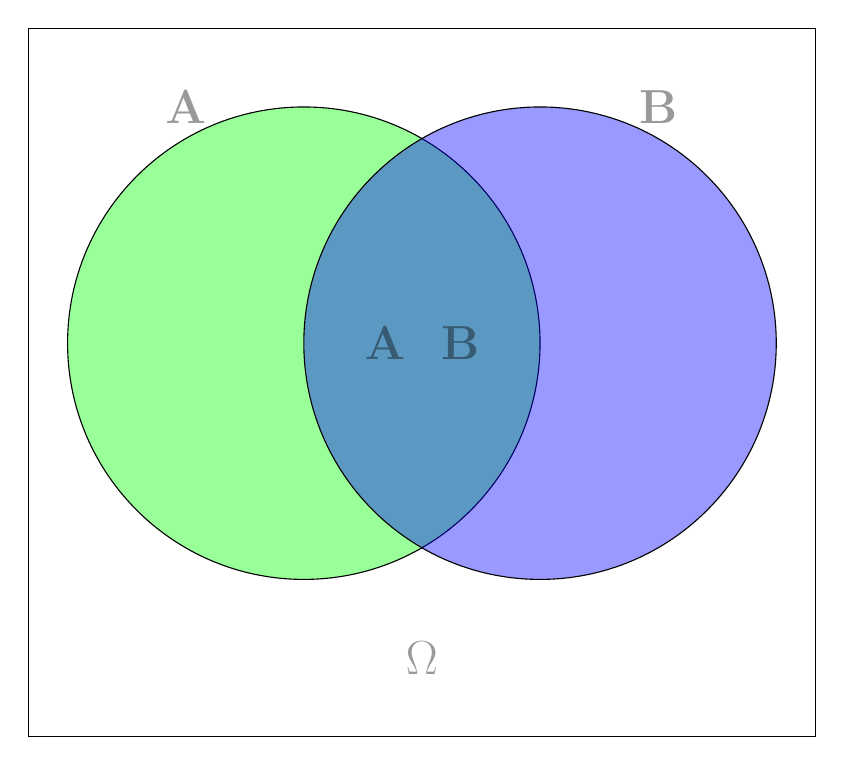
\begin{tikzpicture}
	\begin{scope} [fill opacity = .4]
    \draw (-5,5) rectangle (5,-4);
    \draw[fill=green, draw = black] (-1.5,1) circle (3);
    \draw[fill=blue, draw = black] (1.5,1) circle (3);
    \node at (0,-3) {\LARGE\textbf{$\Omega$}};
    \node at (-3,4) {\LARGE\textbf{A}};
    \node at (3,4) {\LARGE\textbf{B}};
    \node at (0, 1) {\LARGE\textbf{A $\intersect$ B}};
    \end{scope}
\end{tikzpicture}
\end{figure}
We can see from the Venn diagram that the union of two events $A$ and $B$ can be expressed as:
$$A \cup B = A + B - A \cap B$$
Therefore, the probability of the union of two events can be expressed as:
$$P(A \cup B) = P(A) + P(B) - P(A \cap B)$$
Hence proved. For mutually exclusive events, we have $P(A \cap B) = 0$. Therefore, the result follows.
\end{proof}
\begin{corollary}
    In general for events $A_1, A_2, \ldots, A_n$, we have:
    $$P\left( \megaunion{i=1}{n}A_i \right) = \sum_{i=1}^{n} P(A_i) - \sum_{1\leq i < j\leq n} P(A_i \cap A_j) + \sum_{1\leq i < j < k \leq n} P(A_i \cap A_j \cap A_k) - \ldots + (-1)^{n+1}P \left( \megaintersect{i=1}{n}A_i \right)$$
\end{corollary}
\begin{mytheorem}[Probability of the complement of an event]
    Let $A$ be an event. Then, the probability of the complement of $A$, denoted by $A^C$, is given by:
    $$P(A^C) = 1 - P(A)$$
\end{mytheorem}
\begin{proof}
    We have $A \cup A^C = \Omega$ and $A \cap A^C = \emptyset$. Therefore, by the previous theorem, we have:
    $$P(A \cup A^C) = P(A) + P(A^C) - P(A \cap A^C)$$
    $$\implies 1 = P(A) + P(A^C) - 0$$
    $$\implies P(A^C) = 1 - P(A)$$
    Hence proved.
\end{proof}
\begin{mytheorem}[Probability of a subset of an event]
Let $A$ be an event and $B$ be a subset of $A$. Then, the probability of $B$ is given by:
$$P(B) \leq P(A)$$
\end{mytheorem}
\begin{proof}
    We have $B \subseteq A$. Then - \\
    $$A = B \union (A \intersect B^C)$$
    $$\implies P(A) = P(B) + P(A \intersect B^C) \geq P(B)$$
    Hence proved.  
\end{proof}

\begin{mytheorem}[Boole's Inequality]
    Let $A_1, A_2, \ldots, A_n$ be a finite collection of events. Then, the probability of the union of these events is bounded by:
    $$P\left( \megaunion{i=1}{n}A_i \right) \leq \sum_{i=1}^{n} P(A_i)$$
\end{mytheorem}
\begin{proof}
    We prove the above through induction. 
    \textbf{Base Case:} For $n=1$, we have:
    $$P(A_1) \leq P(A_1)$$
    \textbf{Induction Hypothesis:} Assume that the result holds for $n=k$, that is:
    $$P\left( \megaunion{i=1}{k}A_i \right) \leq \sum_{i=1}^{k} P(A_i)$$
    \textbf{Induction Step:} For $n=k+1$, we have:
    \begin{align*}
    P\left( \megaunion{i=1}{k+1}A_i \right) &= P\left( \megaunion{i=1}{k}A_i \cup A_{k+1} \right) \\
    &\leq P\left( \megaunion{i=1}{k}A_i \right) + P(A_{k+1}) \\
    &\leq \sum_{i=1}^{k} P(A_i) + P(A_{k+1}) \\
    &= \sum_{i=1}^{k+1} P(A_i)
    \end{align*}
    Hence proved. 
\end{proof}
\subsection{Conditional Probability}
\begin{mydefinition}{Conditional Probability}
    The conditional probability of an event $A$ given an event $B$ is defined as:
    $$P(A|B) = \frac{P(A \cap B)}{P(B)}$$
    for $P(B) > 0$.
\end{mydefinition}
\begin{example}
    Let $A$ be the event that it rains today, and let $B$ be the event that I carry an umbrella. Then, the conditional probability $P(A|B)$ is the probability that it rains today given that I carry an umbrella.
\end{example}
\begin{example}
    Let $A$ be the event that I study for the exam, and let $B$ be the event that I pass the exam. Then, the conditional probability $P(A|B)$ is the probability that I study for the exam given that I pass the exam.
\end{example}
\begin{mytheorem}[Generalized Bayes' Theorem]
    Let $A_1, A_2, \ldots, A_n$ be a partition of the sample space $\Omega$, and let $B$ be any event such that $P(B) > 0$. Then, the conditional probability of an event $A_i$ given $B$ is given by:
    $$P(A_i|B) = \frac{P(B|A_i)P(A_i)}{\sum_{j=1}^{n} P(B|A_j)P(A_j)}$$
\end{mytheorem}
\begin{proof}
    We have:
    $$P(A_i|B) = \frac{P(B|A_i)P(A_i)}{P(B)}$$
    By the law of total probability, we can express $P(B)$ as:
    $$P(B) = \sum_{j=1}^{n} P(B|A_j)P(A_j)$$
    Therefore, we can rewrite the conditional probability as:
    $$P(A_i|B) = \frac{P(B|A_i)P(A_i)}{\sum_{j=1}^{n} P(B|A_j)P(A_j)}$$
\end{proof}
\begin{mynote}
This proof is not a part of the syllabus, but is included for completeness.
\end{mynote}
\subsection{Independence of Events}
\begin{mydefinition}{Independent Events}
    Two events $A$ and $B$ are said to be independent if the occurrence of one event does not affect the occurrence of the other event. Formally, two events $A$ and $B$ are independent if:
    $$P(A \cap B) = P(A)P(B)$$
    Equivalently, we can say that two events $A$ and $B$ are independent if:
    $$P(A|B) = P(A) \quad \text{and} \quad P(B|A) = P(B)$$
    provided that $P(B) > 0$ and $P(A) > 0$.
\end{mydefinition}
\begin{example}
    Consider the random experiment of rolling a fair six-sided die twice. Let $A$ be the event that the first roll is even, and let $B$ be the event that the second roll is odd. Then, $A$ and $B$ are independent events, since the outcome of the first roll does not affect the outcome of the second roll.
\end{example}
\begin{example}
    Consider the random experiment of drawing 4 subsequent cards from a standard deck of 52 cards without replacement. Let $A$ be the event that the first card is a heart, and let $B$ be the event that the second card is a heart. Then, $A$ and $B$ are \underemphasise{not independent} events, since the outcome of the first draw affects the outcome of the second draw.
\end{example}
\begin{mydefinition}{Pairwise and Mutual Independence}
    \textbf{Pairwise Independence: } A collection of events $\{A_1, A_2, \ldots, A_n\}$ is said to be pairwise independent if every pair of events is independent. That is, for all $i \neq j$:
    $$P(A_i \cap A_j) = P(A_i)P(A_j)$$
    \textbf{Mutual Independence: } A collection of events is said to be mutually independent if every event is independent of the intersection of all the others. That is, for all $k \leq n$:
    $$P(A_1 \cap A_2 \cap \ldots \cap A_k) = P(A_1)P(A_2) \ldots P(A_k)$$
\end{mydefinition}
\begin{example}
    Let $A = \{1, 2 , 3, 4\}$, $B = \{3, 4, 5, 6\}$, $C = \{4, 5, 6, 7\}$ be three events in the sample space $\Omega = \{1, 2, 3, 4, 5, 6, 7, 8\}$. Then, we can see that $A$, $B$ and $C$ are independent when considered together, but not pairwise independent. Let us verify this - \\
    $P(A) = P(B) = P(C) = \frac{4}{8} = \frac{1}{2}$ \\
    $P(A\intersect B) = P(\{3, 4\}) = \frac{2}{8} = \frac{1}{4} = P(A)P(B)$ \\
    $P(A\intersect C) = P(\{4\}) = \frac{1}{8} \neq P(A)P(C)$ \\
    $P(B\intersect C) = P(\{4, 5, 6\}) = \frac{3}{8} \neq P(B)P(C)$ \\
    However, \\
    $P(A\intersect B \intersect C) = P(\{4\}) = \frac{1}{8} = P(A)P(B)P(C)$ \\
    Therefore, the triple product holds while pairwise independence fails. 
\end{example}
\begin{mynote}
    It is important to note that pairwise independence does not imply mutual independence. That is, even if every pair of events in a collection is independent, it does not necessarily mean that the entire collection is mutually independent. Mutual independence is a stronger condition than pairwise independence, and it requires that every event in the collection be independent of the intersection of all the others.
\end{mynote}
\begin{mydefinition}{Conditional Independence}
    Two events $A$ and $B$ are said to be conditionally independent given a third event $C$ if the occurrence of $A$ does not affect the occurrence of $B$ when $C$ has occurred. Formally, $A$ and $B$ are conditionally independent given $C$ if:
    $$P(A \cap B | C) = P(A|C)P(B|C)$$
    provided that $P(C) > 0$.
\end{mydefinition}
\begin{mynote}
    Note that two events being conditionally independent given a third event does not imply that they are independent in general. Conditional independence is a weaker condition than unconditional independence.
\end{mynote}
\section{Different Approaches and Definitions of Probability}
\subsection{Statistical Definition of Probability}
\begin{mydefinition}{Statistical definition of Probability}
    The statistical definition of probability states that the probability of an event is the limit of its relative frequency in a large number of trials. \\
    Let $A$ be an event in the sample space $\Omega$. Let $N$ be the total number of trials of the random experiment, and let $N_A$ be the number of times the event $A$ occurs in these trials. Then, the probability of the event $A$, denoted by $P(A)$, is given by:
    $$P(A) = \lim_{N \to \infty} \frac{N_A}{N}$$
    provided that the limit exists.
\end{mydefinition}
\begin{mynote}
    This definition provides a more reliable foundation for the concept of probability, since with this definition, we will always get the same probability for any event in a sample space. Moreover, it emphasizes the importance of conducting a large number of trials to obtain a stable estimate of probability. We shall prove under the central limit theorem that the distribution of the sample mean approaches a normal distribution as the sample size increases, regardless of the original distribution of the data.
\end{mynote}
\begin{example}
    Consider the random experiment of flipping a fair coin multiple times. Let $A$ be the event that we get heads on the first flip, and let $B$ be the event that we get heads on the second flip. According to the statistical definition of probability, we can estimate $P(A)$ and $P(B)$ by conducting a large number of trials and observing the relative frequencies of heads. It can be empirically verified that the events $A$ and $B$ are independent, since the outcome of the first flip does not affect the outcome of the second flip.
\end{example}


\subsection{Axiomatic Definition of Probability}
\begin{mydefinition}{$\sigma$-field or $\sigma$-algebra}
    A $\sigma$-field (or $\sigma$-algebra) on a set $\Omega$ is a collection $\mathcal{F}$ of subsets of $\Omega$ such that:
    \begin{enumerate}
        \item The empty set is in $\mathcal{F}$: $\emptyset \in \mathcal{F}$.
        \item If $A \in \mathcal{F}$, then its complement is also in $\mathcal{F}$: $A^c \in \mathcal{F}$.
        \item If $A_1, A_2, \ldots \in \mathcal{F}$ are countably many sets, then their union is also in $\mathcal{F}$: $\bigcup_{i=1}^{\infty} A_i \in \mathcal{F}$.
    \end{enumerate}
    In essence, a $\sigma$-field is closed under complementation and countable unions.
\end{mydefinition}
\begin{example}
    Consider the sample space $\Omega$ of all possible outcomes when rolling a fair six-sided die. The $\sigma$-algebra $\mathcal{F}$ generated by this sample space includes all possible subsets of $\Omega$, including the empty set, singletons (e.g., $\{1\}$, $\{2\}$), and the entire sample space itself. This $\sigma$-algebra is closed under complementation and countable unions.
\end{example}
In general, we note that the concept of a $\sigma$-field is fundamental to the axiomatic approach to probability. Every power set of a sample space forms a $\sigma$-field. 
We define here the smallest and largest $\sigma$-field on a sample space $\Omega$:
\begin{itemize}
    \item The smallest $\sigma$-field is the trivial $\sigma$-field, which contains only the empty set and the entire sample space: $\mathcal{F}_{\text{min}} = \{\emptyset, \Omega\}$.
    \item The largest $\sigma$-field is the power set of $\Omega$, which contains all possible subsets of $\Omega$: $\mathcal{F}_{\text{max}} = 2^{\Omega}$.
\end{itemize}
\begin{mydefinition}{Kalmagarov's Definition}
    Let $\Omega$ be a sample space, and let $\mathcal{F}$ be a $\sigma$-algebra of subsets of $\Omega$. A probability measure $P$ is a function that assigns a probability to each event in $\mathcal{F}$ such that the following axioms hold:
    \begin{enumerate}
        \item Non-negativity: For any event $A \in \mathcal{F}$, $P(A) \geq 0$.
        \item Normalization: $P(\Omega) = 1$.
        \item Countable additivity: For any countable collection of disjoint events $A_1, A_2, \ldots \in \mathcal{F}$, we have:
        $$P\left(\bigcup_{i=1}^{\infty} A_i\right) = \sum_{i=1}^{\infty} P(A_i)$$
    \end{enumerate}
    This probability function on $\mathcal{F}$ satisfies the axioms of probability and provides a rigorous foundation for the concept of probability in the context of measure theory. Further, this function is unique. 
\end{mydefinition}
\begin{example}
    Let $\Omega$ be the sample space of rolling a fair six-sided die. The $\sigma$-algebra $\mathcal{F}$ generated by this sample space includes all possible subsets of $\Omega$. A probability measure $P$ can be defined on $\mathcal{F}$ by assigning a probability of $\frac{1}{6}$ to each individual outcome (e.g., $P(\{1\}) = \frac{1}{6}$, $P(\{2\}) = \frac{1}{6}$, etc.) and ensuring that the total probability sums to 1. Note that this construction satisfies all the axioms of a probability measure.
\end{example}

\section{Random Variables and Probability Distributions}
\subsection{Random Variables}
\begin{mydefinition}{Random Variable}
    A random variable is a function that assigns a real number to each outcome in a sample space of a random experiment. Formally, a random variable $X$ is a function from the sample space $\Omega$ to the real numbers $\mathbb{R}$:
    $$X: \Omega \to \mathbb{R}$$
    Random variables can be classified into two main types:
    \begin{itemize}
        \item \textbf{Discrete Random Variables:} These take on a countable number of distinct values. Examples include the outcome of rolling a die or the number of heads in a series of coin flips.
        \item \textbf{Continuous Random Variables:} These can take on any value within a given range or interval. Examples include the height of individuals in a population or the time it takes to complete a task.
    \end{itemize}
\end{mydefinition}
\begin{example}
    Let $X$ be a discrete random variable representing the outcome of rolling a fair six-sided die. The possible values of $X$ are $\{1, 2, 3, 4, 5, 6\}$, each with a probability of $\frac{1}{6}$. The probability mass function (PMF) of $X$ is given by:
    $$P(X = k) = \frac{1}{6}, \quad k \in \{1, 2, 3, 4, 5, 6\}$$
\end{example}
\begin{mydefinition}{Probability Density Function (pdf)}
    A probability density function (pdf) is a function that describes the likelihood of a continuous random variable taking on a particular value. The pdf must satisfy the following properties:
    \begin{itemize}
        \item Non-negativity: $f(x) \geq 0$ for all $x \in \mathbb{R}$.
        \item Normalization: The total area under the curve of the pdf must equal 1:
        $$\int_{-\infty}^{\infty} f(x) \, dx = 1$$
        Alternatively, we can denote the area under the curve by defining the integral to cover the entire sample space - in this case, the range of the continuous random variable.
        $$\int_{\Omega} f(x) \, dx = 1$$
    \end{itemize}
\end{mydefinition}
\begin{mydefinition}{Independence of Random Variables}
    Two random variables $X, Y$ are said to be independent if - 
    $$P(X=i, Y=j) = P(X=i)P(Y=j) \forall i, j$$
\end{mydefinition}
\begin{example}
    Let $X$ be a continuous random variable representing the height of individuals in a population. The probability density function (pdf) of $X$ might be modeled using a normal distribution with a mean $\mu$ and standard deviation $\sigma$. The pdf is given by:
    $$f(x) = \frac{1}{\sigma \sqrt{2\pi}} e^{-\frac{(x - \mu)^2}{2\sigma^2}}$$
    The area under the curve of this pdf over the entire real line is equal to 1, satisfying the normalization condition.
\end{example}
\begin{example}
    Let $X$ be a continuous random variable representing the time it takes for a computer to complete a task. The probability density function (pdf) of $X$ might be modeled using an exponential distribution with a rate parameter $\lambda$. The pdf is given by:
    $$f(x) = \lambda e^{-\lambda x}, \quad x \geq 0$$
    The area under the curve of this pdf over the entire real line is equal to 1, satisfying the normalization condition.
\end{example}
\begin{mydefinition}{Cumulative Distribution Function (cdf)}
    The cumulative distribution function (cdf) of a random variable $X$ is a function that gives the probability that $X$ takes on a value less than or equal to a given value $x$. The cdf is defined as:
    $$F(x) = P(X \leq x) = \int_{-\infty}^{x} f(t) \, dt$$
    The cdf has the following properties:
    \begin{itemize}
        \item Non-decreasing: $F(x)$ is a non-decreasing function of $x$.
        \item Limits: $\lim_{x \to -\infty} F(x) = 0$ and $\lim_{x \to \infty} F(x) = 1$.
        \item Right-continuous: $F(x)$ is right-continuous, meaning that for any $x_0$, $\lim_{x \to x_0^+} F(x) = F(x_0)$.
    \end{itemize}
    For a discrete random variable, we may define the cdf as follows:
    $$F(x) = \sum_{k \leq x} P(X = k)$$
\end{mydefinition}
\begin{example}
    Let $X$ be a discrete random variable representing the outcome of rolling a fair six-sided die. The cumulative distribution function (cdf) of $X$ is given by:
    \[
    F(x) = 
    \begin{cases} 
    0 & x < 1 \\
    \frac{1}{6} & 1 \leq x < 2 \\
    \frac{2}{6} & 2 \leq x < 3 \\
    \frac{3}{6} & 3 \leq x < 4 \\
    \frac{4}{6} & 4 \leq x < 5 \\
    \frac{5}{6} & 5 \leq x < 6 \\
    1 & x \geq 6 
    \end{cases}
    \]
    This cdf gives the probability that the outcome of rolling the die is less than or equal to a given value $x$.
\end{example}
\begin{example}
    Let $X$ be a continuous random variable representing the time it takes for a computer to complete a task. The cumulative distribution function (cdf) of $X$ is given by:
    $$F(x) = P(X \leq x) = \int_{0}^{x} f(t) \, dt$$
    where $f(t) = e^{-\lambda t}$ is the probability density function (pdf) of $X$. The cdf gives the probability that the time taken to complete the task is less than or equal to a given value $x$.
    $$F(x) = 1 - e^{-\lambda x}$$ 
\end{example}

\subsection{Expectation and Variance of a Random Variable}
\begin{mydefinition}{Expectation or Expected Value}
    The expectation (or expected value) of a random variable $X$, denoted by $E(X)$ or $\mu_X$, is a measure of the central tendency of the random variable. It is defined as follows:
    \begin{itemize}
        \item For a discrete random variable:
        $$E(X) = \sum_{x} x P(X = x)$$
        where the sum is taken over all possible values of $X$.
        \item For a continuous random variable:
        $$E(X) = \int_{-\infty}^{\infty} x f(x) \, dx$$
        where $f(x)$ is the probability density function (pdf) of $X$.
    \end{itemize}
    $E(X)$ has the following properties:
    \begin{itemize}
        \item Linearity: For any constants $a$ and $b$, $E(aX + b) = aE(X) + b$.
        \item Non-negativity: If $X \geq 0$, then $E(X) \geq 0$.
        \item Additivity: For any two random variables $X$ and $Y$, $E(X + Y) = E(X) + E(Y)$.
    \end{itemize}
\end{mydefinition}
\textbf{Physical Interpretation of Expectation} - The expectation of a random variable can be thought of as the long-term average value of the random variable over many trials of the random experiment. It provides a measure of the "center" or "typical" value of the random variable. It is known as the mean of the distribution.
\begin{figure}[H]
    \centering
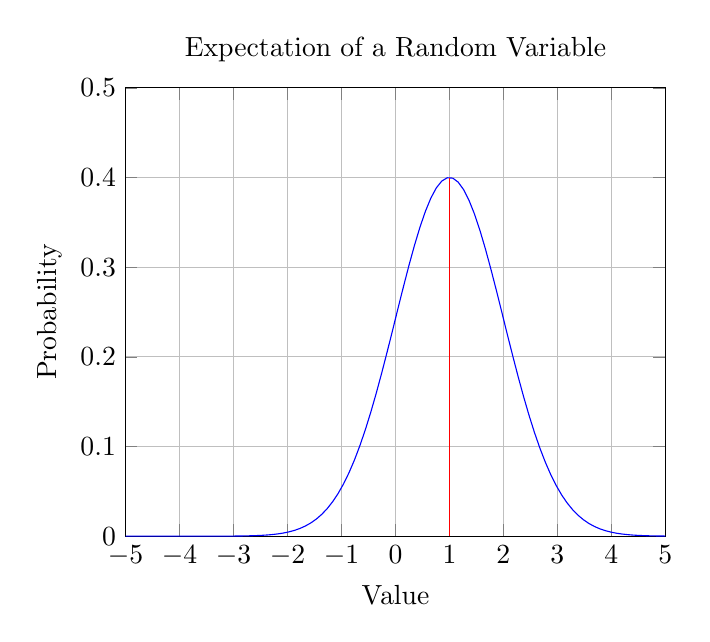
\begin{tikzpicture}
    \begin{axis}[
        title={Expectation of a Random Variable},
        xlabel={Value},
        ylabel={Probability},
        xmin=-5, xmax=5,
        ymin=0, ymax=0.5,
        xtick={-5,-4,...,5},
        ytick={0,0.1,...,0.5},
        grid=major
    ]
    \addplot[
        domain=-5:5, 
        samples=100, 
        color=blue,
    ]
    {0.4*exp(-0.5*(x-1)^2)};
    %the mean is - 1
    \addplot[color=red] coordinates {(1, 0) (1, 0.4)};
    \end{axis}
\end{tikzpicture}
\label{fig:expectation}
\caption{Expectation of a Random Variable}
\end{figure}
In the given figure, the expectation tells us whether the random variable is more likely to take on values greater than or less than 1 (the peak). If the expectation is greater than 1, it indicates that the random variable is more likely to take on values greater than 1, and vice versa. 

\begin{mydefinition}{Riemann-Steltjes Integral}
    If $f$ is a pdf of a random variable $X$ and $g$ is a well behaved function (i.e. it does not have discontinuities or singularities in the range of $X$), then the expectation of $g(X)$ is given by:
    \begin{itemize}
        \item For a discrete random variable:
        $$E(g(X)) = \sum_{x} g(x) P(X = x)$$
        where the sum is taken over all possible values of $X$.
        \item For a continuous random variable:
        $$E(g(X)) = \int_{-\infty}^{\infty} g(x) f(x) \, dx$$
        where $f(x)$ is the probability density function (pdf) of $X$.
    \end{itemize}
    Provided that $E(|g(X)|) < \infty$, i.e., $$\int_{-\infty}^{\infty} |g(x)| f(x) \, dx < \infty$$
\end{mydefinition}
\begin{mydefinition}{Variance}
    The variance of a random variable $X$, denoted by $\text{Var}(X)$, is a measure of the dispersion or spread of the random variable's possible values. It is defined as follows:
    \begin{itemize}
        \item For a discrete random variable:
        $$\text{Var}(X) = E(X^2) - (E(X))^2$$
        where $E(X^2)$ is the expected value of the square of $X$.
        \item For a continuous random variable:
        $$\text{Var}(X) = \int_{-\infty}^{\infty} x^2 f(x) \, dx - (E(X))^2$$
        where $f(x)$ is the probability density function (pdf) of $X$.
    \end{itemize}
\end{mydefinition}

\textbf{Physical Interpretation of Variance} - The variance provides a measure of how much the values of a random variable differ from the expected value. A low variance indicates that the values tend to be close to the mean, while a high variance indicates that the values are spread out over a wider range. Variation is \underemphasise{Measure of Dispersion}.
\begin{mydefinition}{Moments}
    \begin{enumerate}
    \item The $n$-th order raw moment of a random variable $X$ is defined as:
    \begin{itemize}
        \item For a discrete random variable:
        $$E(X^n) = \sum_{x} x^n P(X = x)$$
        \item For a continuous random variable:
        $$E(X^n) = \int_{-\infty}^{\infty} x^n f(x) \, dx$$
    \end{itemize}
    \item The $n$-th order central moment of a random variable $X$ is defined as:
    \begin{itemize}
    \item For discrete random variables: 
    $$E((X - E(X))^n) = \sum_{x} (x - E(X))^n P(X = x)$$
    \item For continuous random variables:
    $$E((X - E(X))^n) = \int_{-\infty}^{\infty} (x - E(X))^n f(x) \, dx$$
    \end{itemize}
    
    \item The $n^th$ order raw moment about a point $c$ is defined as:
    \begin{itemize}
        \item For discrete random variables:
        $$E((X - c)^n) = \sum_{x} (x - c)^n P(X = x)$$
        \item For continuous random variables:
        $$E((X - c)^n) = \int_{-\infty}^{\infty} (x - c)^n f(x) \, dx$$
    \end{itemize}
    \end{enumerate}
\end{mydefinition}
\textbf{Physical Interpretation of Moments} - The moments of a random variable provide important information about its distribution. The raw moments give a sense of the "size" of the values, while the central moments (like variance) provide insight into the "spread" or "variability" of the distribution.
The moments about a point provide information about the shape of the distribution relative to that point. 


\begin{mytheorem}[Cauchy-Schwarz Inequality]
For any random variables $X$ and $Y$ with finite expectations, the following inequality holds:
$$E(XY) \leq E(X^2)^{1/2} E(Y^2)^{1/2}$$
\end{mytheorem}
\begin{proof}
    Let $\lambda \in \R$ be a constant. Let the pdf of $X$ be $f(x)$ and $Y$ be $g(x)$. We have: 
    $$E(f(x) + \lambda(g(x)))^2 \geq 0$$
    \begin{align*}
        &\implies E(f(x)^2 + 2\lambda f(x)g(x) + \lambda^2 g(x)^2) \geq 0 \\
        &\implies E(f(x)^2) + 2\lambda E(f(x)g(x)) + \lambda^2 E(g(x)^2) \geq 0 \\
    \end{align*}
    This is a quadratic inequality in $\lambda$, and it must hold for all $\lambda \in \R$. Therefore, the discriminant of this quadratic must be non-positive:
    $$D = (2E(f(x)g(x)))^2 - 4E(f(x)^2)E(g(x)^2) \leq 0$$
    which implies the Cauchy-Schwarz inequality.
\end{proof}
\subsection{Special Moments}
\begin{mydefinition}{Skewness}
    Skewness is a measure of the asymmetry of the probability distribution of a real-valued random variable about its mean. It is defined as the third standardized moment:
    $$\mu_3(X) = E((X - E(X))^3)$$
    We cannot standardize its units like we do for variance, because the cube root of variance does not have a meaningful interpretation.
    The skewness is then given by:
    $$\text{Skewness}(X) = \frac{E((X - E(X))^3)}{(E((X - E(X))^2))^{3/2}}$$
    or alternatively, we write - 
    $$\gamma_1 = \frac{\mu_3(X)}{(\mu_2(X))^{3/2}}$$
    where $E(X)$ is the expectation of $X$ and $E((X - E(X))^2)$ is the variance of $X$.
    We also define - 
    $$\beta_1 = \gamma_1^2 = \frac{(\mu_3(X))^2}{(\mu_2(X))^3}$$
\end{mydefinition}
\textbf{Physical Interpretation of Skewness} - Skewness provides insight into the shape of the distribution. A positive skew indicates that the right tail is longer or fatter than the left tail, while a negative skew indicates that the left tail is longer or fatter than the right tail. A skewness of zero indicates a symmetric distribution.
\begin{mydefinition}{Kurtosis}
    Kurtosis is a measure of the "tailedness" of the probability distribution of a real-valued random variable. It is defined as the fourth standardized moment:
    $$\text{Kurtosis}(X) = \frac{E((X - E(X))^4)}{(E((X - E(X))^2))^2}$$
    where $E(X)$ is the expectation of $X$ and $E((X - E(X))^2)$ is the variance of $X$.
    We denote kurtosis by $\beta_2$:
    $$\beta_2 = \frac{\mu_4(X)}{(\mu_2(X))^2}$$
    where $\mu_4(X) = E((X - E(X))^4)$ is the fourth central moment of $X$.
\end{mydefinition}
\textbf{Physical Interpretation of Kurtosis} - Kurtosis provides insight into the shape of the distribution, particularly in terms of the presence of outliers.
A higher kurtosis indicates that the distribution has heavier tails and a sharper peak compared to a normal distribution, while a lower kurtosis indicates lighter tails and a flatter peak.
\begin{mynote}
    The kurtosis of a normal distribution is 3. To compare the kurtosis of a distribution to that of a normal distribution, we often use the excess kurtosis, which is defined as:
    $$\text{Excess Kurtosis} = \beta_2 - 3$$
    A positive excess kurtosis indicates a distribution with heavier tails than a normal distribution, while a negative excess kurtosis indicates lighter tails.
    We also divide distributions into three categories based on their kurtosis:
    \begin{itemize}
        \item \textbf{Leptokurtic:} Distributions with positive excess kurtosis (i.e., $\beta_2 > 3$). These distributions have heavier tails and a sharper peak compared to a normal distribution.
        \item \textbf{Platykurtic:} Distributions with negative excess kurtosis (i.e., $\beta_2 < 3$). These distributions have lighter tails and a flatter peak compared to a normal distribution.
        \item \textbf{Mesokurtic:} Distributions with zero excess kurtosis (i.e., $\beta_2 = 3$). The normal distribution is an example of a mesokurtic distribution.
    \end{itemize}
\end{mynote}
\begin{mytheorem}[$\beta_2 \geq 1$]
    For any random variable $X$, the kurtosis $\beta_2$ satisfies the inequality:
    $$\beta_2 \geq 1$$
\end{mytheorem}
\begin{proof}
    Let $g(x) = (x - E(X))^2$ and $h(x) = 1$. Applying the Cauchy-Schwarz inequality, we have:
    $$E(g(x)h(x))^2 \leq E(g(x)^2)E(h(x)^2)$$
    This simplifies to:
    $$E((X - E(X))^2)^2 \leq E((X - E(X))^4)$$
    Dividing both sides by $E((X - E(X))^2)^2$, we get:
    $$1 \leq \frac{E((X - E(X))^4)}{(E((X - E(X))^2))^2} = \beta_2$$
    Hence proved.
\end{proof}
\begin{mynote}
    This theorem implies that the kurtosis of any distribution is always greater than or equal to 1. A kurtosis of 1 corresponds to a distribution with no variability (i.e., all values are the same), while higher kurtosis values indicate increasing levels of variability and the presence of outliers. \\
    A distribution with $\beta_2 = 1$ is a degenerate distribution, where all the probability mass is concentrated at a single point. This means that there is no variability in the data, and every observation is identical. An example of such a distribution is a random variable that always takes the same value, say $c$. In this case, the pdf can be represented as a Dirac delta function centered at $c$, and the variance (and hence kurtosis) is zero.
\end{mynote}
\begin{mytheorem}[$\beta_1 \leq \beta_2$]
    For any random variable $X$, the skewness $\beta_1$ is less than or equal to the kurtosis $\beta_2$:
    $$\beta_1 \leq \beta_2$$
\end{mytheorem}
\begin{proof}
    Let $g(x) = (x - E(x))^2$ and $h(x) = (x - E(x))$. Applying the Cauchy-Schwarz inequality, we have:
    $$E(g(x)h(x))^2 \leq E(g(x)^2)E(h(x)^2)$$
    $$\implies E((X - E(X))^3)^2 \leq E((X - E(X))^4)E((X - E(X))^2)$$
    Dividing both sides by $E((X - E(X))^2)^3$, we get:
    $$\frac{E((X - E(X))^3)^2}{(E((X - E(X))^2))^3} \leq \frac{E((X - E(X))^4)}{(E((X - E(X))^2))^2}$$
    $$\implies \beta_1 \leq \beta_2$$
\end{proof}
\begin{mynote}
    This theorem implies that the skewness of any distribution is always less than or equal to its kurtosis. This relationship provides insight into the shape of the distribution, as skewness measures asymmetry while kurtosis measures the "tailedness" or presence of outliers. A distribution with high skewness is likely to have high kurtosis, but a distribution with low skewness can still have high kurtosis if it has heavy tails.
\end{mynote} 

%\begin{mytheorem}[$\beta_2 \geq \beta_1 + 1$]
    %For any random variable $X$, the kurtosis $\beta_2$ is greater than or equal to the skewness $\beta_1$ plus 1:
    %$$\beta_2 \geq \beta_1 + 1$$
%\end{mytheorem}
%\begin{proof}
 %   Let $g(X) = \frac{(X - E(X))^2 - \mu_2}{\sqrt{E((X^2 - \mu_2)^2)}}$ and $h(X) = \frac{(X - E(X))}{\sqrt{\mu_2}}$. Applying the Cauchy-Schwarz inequality, we have:
  %  $$E(g(X)h(X))^2 \leq E(g(X)^2)E(h(X)^2)$$
   % This simplifies to:
    %$$E\left(\frac{(X - E(X))^3 - \mu_2(X - E(X))}{\sqrt{E((X^2 - \mu_2)^2)\mu_2}}\right)^2 \leq 1$$
    %Expanding the left-hand side, we get:
    %$$E\left((X - E(X))^3 - \mu_2(X - E(X))\right)^2 \leq E((X - E(X))^4)\mu_2$$
%    Expanding the left-hand side further, we have:
 %   $$E((X - E(X))^6) - 2\mu_2 E((X - E(X))^4) + \mu_2^2 E((X - E(X))^2) \leq E((X -% E(X))^4)\mu_2$$
   % Rearranging the terms, we get:
    %$$E((X - E(X))^6) + \mu_2^2 E((X - E(X))^2) \leq 3\mu_2 E((X - E(X))^4)$$
%    Dividing both sides by $\mu_2^3$, we obtain:
 %   $$\frac{E((X - E(X))^6)}{\mu_2^3} + 1 \leq 3\frac{E((X - E(X))^4)}{\mu_2^2}$$
  %  $$\implies \beta_2 \geq \beta_1 + 1$$ 
%\end{proof}

\subsection{Moment Generating Function}
\begin{mydefinition}{Moment Generating Function (MGF)}
    The moment generating function (MGF) of a random variable $X$ is a function that encodes the moments of the random variable. It is defined as:
    $$M_X(t) = E(e^{tX})$$
    where $t$ is a real number. The MGF has the following properties:
    \begin{itemize}
        \item The MGF exists for all $t$ in an open interval containing 0.
        \item The $n$-th moment of $X$ can be obtained by taking the $n$-th derivative of the MGF and evaluating it at $t = 0$:
        $$E(X^n) = M_X^{(n)}(0)$$
        where $M_X^{(n)}(t)$ denotes the $n$-th derivative of $M_X(t)$ with respect to $t$.
        \item If two random variables have the same MGF, they have the same distribution.
    \end{itemize}
\end{mydefinition}
\begin{mytheorem}[$n^{th}$ Derivative of MGF gives $n^{th}$ Moment]
    The $n$-th moment of a random variable $X$ can be obtained by taking the $n$-th derivative of the moment generating function (MGF) and evaluating it at $t = 0$:
    $$E(X^n) = M_X^{(n)}(0)$$
    where $M_X^{(n)}(t)$ denotes the $n$-th derivative of $M_X(t)$ with respect to $t$.
\end{mytheorem}
\begin{proof}
    Let $\mu_x = \int_{\-\infty}^{\infty}e^{tx}f(x) \, dx$ be the MGF of $X$. We have:
    \begin{align*}
        \frac{d^n \mu_x}{dt^n} &= \frac{d^n}{dt^n} \int_{-\infty}^{\infty} e^{tx} f(x) \, dx \\
        &= \int_{-\infty}^{\infty} \frac{d^n}{dt^n} e^{tx} f(x) \, dx \quad \text{(by Leibniz's rule)} \\
        &= \int_{-\infty}^{\infty} x^n e^{tx} f(x) \, dx
    \end{align*}
    Evaluating this at $t = 0$, we get:
    $$\frac{d^n \mu_x}{dt^n} \bigg|_{t=0} = \int_{-\infty}^{\infty} x^n f(x) \, dx = E(X^n)$$
    Hence proved.
\end{proof}
\begin{mynote}
There are some distributions for which the MGF does not exist for all values of $t$. It is important to check the existence of the MGF before using it to derive moments or other properties of the distribution. Therefore, there are some distributions for which some moments may not exist even if the MGF exists. For example, the Cauchy distribution has an MGF that exists for all $t$, but it does not have a defined mean or variance.
\end{mynote}
\begin{example}{Cauchy Distribution}
    The Cauchy distribution is a continuous probability distribution that is often used in statistics and physics. It is characterized by its location parameter $x_0$ and scale parameter $\gamma$. The probability density function (pdf) of the Cauchy distribution is given by:
    $$f(x; x_0, \gamma) = \frac{1}{\pi \gamma \left[1 + \left(\frac{x - x_0}{\gamma}\right)^2\right]}$$
    for $-\infty < x < \infty$, where $x_0$ is the location parameter (the peak of the distribution) and $\gamma$ is the scale parameter (which determines the width of the distribution). The Cauchy distribution has heavy tails, meaning that it has a higher probability of extreme values compared to other distributions like the normal distribution. This makes it useful for modeling phenomena with outliers or extreme events.
    The MGF of the Cauchy distribution does not exist for any value of $t$, which means that we cannot use the MGF to derive moments or other properties of the distribution. In fact, the Cauchy distribution does not have a defined mean or variance, as these moments do not converge.
    \begin{figure}[H]
    \centering
    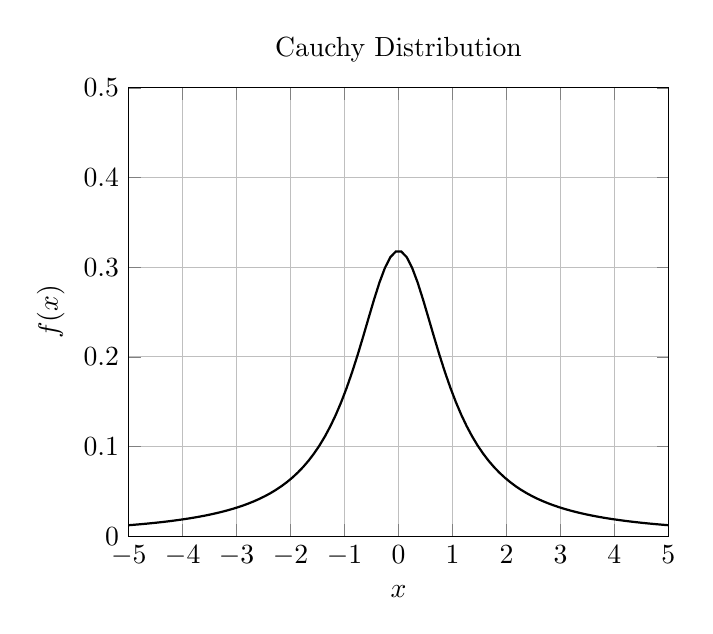
\begin{tikzpicture}
    \begin{axis}
        [title={Cauchy Distribution},
        xlabel={$x$},
        ylabel={$f(x)$},
        xmin=-5, xmax=5,
        ymin=0, ymax=0.5,
        xtick={-5,-4,...,5},
        ytick={0,0.1,...,0.5},
        grid=major
    ]
    \addplot[domain=-5:5, samples=100, thick]{1/(pi*(1+x^2))};
    \end{axis}
    \end{tikzpicture}
    \caption{Cauchy Distribution with $x_0 = 0$ and $\gamma = 1$}
    \end{figure}
\end{example}
\chapter{Probability Distributions}
\section{Discrete Probability Distributions}
\subsection{Bernoulli Distribution}
\begin{mydefinition}{Bernoulli Trials}
    A Bernoulli trial is a random experiment that has exactly two possible outcomes, typically referred to as "success" and "failure". The probability of success is denoted by $p$, while the probability of failure is denoted by $q = 1 - p$. Each trial is independent of the others, meaning that the outcome of one trial does not affect the outcome of any other trial. Therefore a Bernoulli trial has the following properties: 
    \begin{itemize}
        \item There are only two possible outcomes: success (with probability $p$) and failure (with probability $q = 1 - p$).
        \item The trials are independent, meaning that the outcome of one trial does not affect the outcome of any other trial.
        \item The probability of success $p$ remains constant for each trial.
    \end{itemize}
\end{mydefinition}
\begin{example}
    Consider a random experiment of flipping a fair coin. Let $X$ be a Bernoulli random variable that represents the outcome of the coin flip, where $X = 1$ if the result is heads (success) and $X = 0$ if the result is tails (failure). The probability of success (getting heads) is $p = 0.5$, and the probability of failure (getting tails) is $q = 0.5$. The PMF of $X$ is given by:
    $$P(X = x) = 
    \begin{cases} 
    0.5 & \text{if } x = 1 \\
    0.5 & \text{if } x = 0 
    \end{cases}$$
\end{example}
\begin{mydefinition}{Binomial Distribution}
    A Binomial distribution is a discrete probability distribution that describes the number of successes in a fixed number of independent Bernoulli trials. It is characterized by two parameters: $n$, the number of trials, and $p$, the probability of success in each trial. The probability mass function (PMF) of a Binomial random variable $X$ is given by:
    $$P(X = k) = \binom{n}{k} p^k (1 - p)^{n - k}$$
    for $k = 0, 1, 2, \ldots, n$, where $\binom{n}{k}$ is the binomial coefficient representing the number of ways to choose $k$ successes in $n$ trials.
\end{mydefinition}
\begin{example}
    Let us consider a random experiment of rolling a fair six-sided die $n = 10$ times. Let $X$ be a Binomial random variable that represents the number of times we get a 6 (success) in these 10 rolls. The probability of success (getting a 6) is $p = \frac{1}{6}$, and the probability of failure (not getting a 6) is $q = 1 - p = \frac{5}{6}$. The PMF of $X$ is given by:
    $$P(X = k) = \binom{10}{k} \left(\frac{1}{6}\right)^k \left(\frac{5}{6}\right)^{10 - k}$$
    for $k = 0, 1, 2, \ldots, 10$. For example, the probability of getting exactly 3 sixes in 10 rolls is:
    \begin{align*}
        P(X = 3) &= \binom{10}{3} \left(\frac{1}{6}\right)^3 \left(\frac{5}{6}\right)^{7} \\
        &= 120 \cdot \frac{1}{216} \cdot \frac{78125}{279936} \\
        &\approx 0.155
    \end{align*}
    Let us plot the PMF of $X$ for $k = 0, 1, 2, \ldots, 10$.
    \begin{figure}[H]
    \centering
    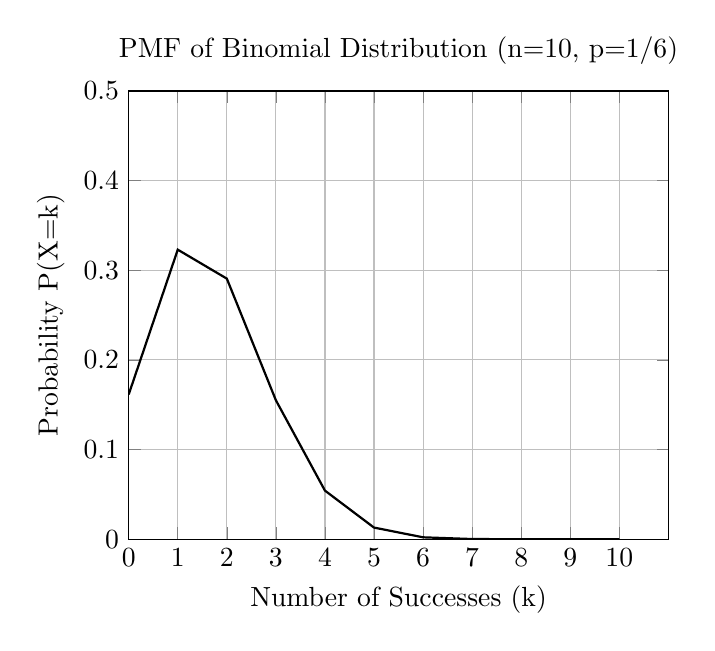
\begin{tikzpicture}
    \begin{axis}[
        title={PMF of Binomial Distribution (n=10, p=1/6)},
        xlabel={Number of Successes (k)},
        ylabel={Probability P(X=k)},
        xmin=0, xmax=11,
        ymin=0, ymax=0.5,
        xtick={0,1,...,10},
        ytick={0,0.1,...,0.5},
        grid=major
    ]
    \addplot[
        domain=0:10,
        samples=11, 
        thick
    ]
    {factorial(10)/(factorial(x)*factorial(10-x))*(1/6)^x*(5/6)^(10-x)};
    \end{axis}
    \end{tikzpicture}
    \caption{PMF of Binomial Distribution with $n=10$ and $p=\frac{1}{6}$}
    \end{figure}
\end{example}

\begin{mytheorem}[Sum of PMF of Binomial Distribution is 1]
    The sum of the probabilities in the probability mass function (PMF) of a Binomial distribution is equal to 1. That is, for a Binomial random variable $X$ with parameters $n$ and $p$, we have:
    $$\sum_{k=0}^{n} P(X = k) = 1$$
    We define $P(X = k)$ as:
    $$P(X = k) = \binom{n}{k} p^k (1 - p)^{n - k}$$
\end{mytheorem}
\begin{proof}
    Suppose we have $n$ independent Bernoulli trials, each with a probability of success $p$ and a probability of failure $1 - p$. The random variable $X$ represents the number of successes in these $n$ trials. We consider the probability of getting exactly $k$ successes in $n$ trials. Let the outcomes be represented by a sequence of $n$ trials, where each trial can result in either a success (S) or a failure (F). The number of ways to arrange $k$ successes and $n - k$ failures in $n$ trials is given by the binomial coefficient $\binom{n}{k}$. The probability of getting exactly $k$ successes and $n - k$ failures in a specific arrangement is given by $p^k (1 - p)^{n - k}$. Therefore, the probability of getting exactly $k$ successes in $n$ trials is given by:
    $$P(X = k) = \binom{n}{k} p^k (1 - p)^{n - k}$$
    To show that the sum of the probabilities in the PMF is equal to 1, we sum $P(X = k)$ over all possible values of $k$ from 0 to $n$:
    \begin{align*}
        \sum_{k=0}^{n} P(X = k) &= \sum_{k=0}^{n} \binom{n}{k} p^k (1 - p)^{n - k} \\
        &= (p + (1 - p))^n \quad \text{(by the Binomial Theorem)} \\
        &= 1^n \\
        &= 1
    \end{align*}
    Hence proved.
\end{proof}

\subsubsection{Expectation of a Random Variable following Bernoulli Distribution}
Let $X$ be a random variable following a Bernoulli distribution with probability of success $p$. Let $N$ denote the number of independent trials. Let $k$ denote the number of successes in these $N$ trials. Then, the expectation of $X$ is given by:
\begin{align*}
    E(X) &= \sum_{k=1}^{N} k P(X = k) \\
    &= \sum_{k=1}^{N} k \binom{N}{k} p^k (1 - p)^{N - k} \\
    &= \sum_{k=1}^{N} k\cdot \frac{N!}{k!(N-k)!} p^k (1 - p)^{N - k} \\
    &= \sum_{k=1}^{N} \frac{N!}{(k-1)!(N-k)!} p^k (1 - p)^{N - k} \\
    &= \sum_{k=1}^{N} N \cdot \frac{(N-1)!}{(k-1)!((N-1)-(k-1))!} p^k (1 - p)^{N - k} \\
    &= Np \sum_{k=1}^{N} \binom{N-1}{k-1} p^{k-1} (1 - p)^{(N-1) - (k-1)} \\
    &= Np
\end{align*}
\subsubsection{Variance of a Random Variable following Bernoulli Distribution}
We can calculate the variance and other moments of any distribution by differentiating the moment generating function (MGF). We can define the MGF of a Bernoulli distribution as follows:
\begin{align*}
    M_X(t) &= E(e^{tX}) \\
    &= \sum_{k=0}^{N} e^{tk} P(X = k) \\
    &= \sum_{k=0}^{N} e^{tk} \binom{N}{k} p^k (1 - p)^{N - k} \\
    &= \sum_{k=0}^{N} \binom{N}{k} (pe^t)^k (1 - p)^{N - k} \\
    &\boxed{=(pe^t + (1 - p))^N}
\end{align*}
The variance of a random variable $X$ following a Bernoulli distribution with probability of success $p$ is given by:
\begin{figure}[H]
\begin{align*}
    \mu_2(X) &= E((X - np)^2) \\
    &= \sum_{k=0}^{N} (k - np)^2 P(X = k) \\
    &= \sum_{k=0}^{N} (k - np)^2 \binom{N}{k} p^k (1 - p)^{N - k} \\
    &= \sum_{k=0}^{N} (k^2 - 2knp + n^2p^2) \binom{N}{k} p^k (1 - p)^{N - k} \\
    &= \left(\sum_{k=0}^{N} k^2 \binom{N}{k} p^k (1 - p)^{N - k}\right) - \left(2np \sum_{k=0}^{N} k \binom{N}{k} p^k (1 - p)^{N - k}\right) + \left(n^2p^2 \sum_{k=0}^{N} \binom{N}{k} p^k (1 - p)^{N - k}\right) \\
    &= \left(\sum_{k=0}^{N} k^2 \binom{N}{k} p^k (1 - p)^{N - k}\right) - 2np(np) + n^2p^2 \cdot 1 \\
    &= \left(\sum_{k=0}^{N} k^2 \binom{N}{k} p^k (1 - p)^{N - k}\right) - n^2p^2 \\
    &= \left(\sum_{k=0}^{N} k(k-1) \binom{N}{k} p^k (1 - p)^{N - k}\right) + \left(\sum_{k=0}^{N} k \binom{N}{k} p^k (1 - p)^{N - k}\right) - n^2p^2 \\
    &= \left(\sum_{k=0}^{N} k(k-1) \binom{N}{k} p^k (1 - p)^{N - k}\right) + np - n^2p^2 \\
    &= \left(\sum_{k=0}^{N} \frac{N!}{(k-2)!(N-k)!} p^k (1 - p)^{N - k}\right) + np - n^2p^2 \\
    &= \left(\sum_{k=0}^{N} N(N-1) \cdot \frac{(N-2)!}{(k-2)!((N-2)-(k-2))!} p^k (1 - p)^{N - k}\right) + np - n^2p^2 \\
    &= \left(N(N-1)p^2 \sum_{k=0}^{N} \binom{N-2}{k-2} p^{k-2} (1 - p)^{(N-2) - (k-2)}\right) + np - n^2p^2 \\
    &= N(N-1)p^2 + np - n^2p^2 \\
    &= Np(1-p)
\end{align*}
\end{figure}
\begin{mynote}
    There are multiple ways to derive the variance of a Bernoulli distribution. One common method is to use the formula for variance in terms of expectation:
    $$\text{Var}(X) = E(X^2) - (E(X))^2$$
    We already know that $E(X) = Np$. To find $E(X^2)$, we can use the fact that for a Bernoulli random variable, $X^2 = X$ (since $X$ can only take values 0 or 1). Therefore, $E(X^2) = E(X) = Np$. Substituting these values into the variance formula, we get:
    \begin{align*}
        \text{Var}(X) &= E(X^2) - (E(X))^2 \\
        &= Np - (Np)^2 \\
        &= Np(1 - p)
    \end{align*}
    Hence, we arrive at the same result for the variance of a Bernoulli distribution.
\end{mynote}
\subsubsection{The $r^{th}$ Moment of a Random Variable following Bernoulli Distribution}
The $r^{th}$ moment of a random variable $X$ following a Bernoulli distribution with probability of success $p$ is given by:
\begin{figure}[H]
\begin{align*}
    \mu_r(X) &= E((X - np)^r) \\
    &= \sum_{k=0}^{N} (k - np)^r P(X = k) \\
    \implies \frac{d\mu_r(X)}{dp} &= \sum_{k=0}^{N} \frac{d}{dp} \left((k - np)^r P(X = k)\right) \\
    &= \sum_{k=0}^{N} \left(r(k - np)^{r-1}(-n) P(X = k) + (k - np)^r \frac{dP(X = k)}{dp}\right) \\
    &= -nr \sum_{k=0}^{N} (k - np)^{r-1} P(X = k) + \sum_{k=0}^{N} (k - np)^r \frac{dP(X = k)}{dp} \\
    &= -nr \mu_{r-1}(X) + \frac{1}{p(1-p)}(\mu_{r+1}(X) + 1) \\
    \implies \mu_{r+1}(X) &= p(1-p)\frac{d\mu_r(X)}{dp} + nrp(1-p)\mu_{r-1}(X)
\end{align*}
\end{figure}
Therefore, we have - 
\begin{figure}[H]
\begin{align*}
    \mu_3 &= np(1-p)(p-(1-p)) \\
    \mu_4 &= 3n^2P^2(1-p)^2 + np(1-p)(1-6p(1-p)) \\
    \implies \gamma_1 &= \frac{1-2p}{\sqrt{np(1-p)}} \\
    \implies \gamma_2 &= \frac{1-6p(1-p)}{np(1-p)} \\
    \implies \beta_1 &= \frac{(1-2p)^2}{np(1-p)} \\
    \implies \beta_2 &= 3 + \frac{1-6p(1-p)}{np(1-p)} \\ 
\end{align*}
\end{figure}
\subsubsection{Conditions for kurtosis of a Bernoulli Distribution to be less than, equal to or greater than 3}
The kurtosis $\beta_2$ of a Bernoulli distribution is given by:
$$\beta_2 = 3 + \frac{1 - 6p(1-p)}{np(1-p)}$$
To determine the conditions under which the kurtosis is less than, equal to, or greater than 3, we analyze the term $\frac{1 - 6p(1-p)}{np(1-p)}$:
\begin{itemize}
    \item \textbf{Kurtosis less than 3:} 
    $$\beta_2 < 3 \implies \frac{1 - 6p(1-p)}{np(1-p)} < 0 \implies 1 - 6p(1-p) < 0 \implies p(1-p) > \frac{1}{6}$$
    The maximum value of $p(1-p)$ is $\frac{1}{4}$, which occurs at $p = \frac{1}{2}$. Therefore, there are no values of $p$ in the interval $[0, 1]$ such that $p(1-p) > \frac{1}{6}$. Hence, the kurtosis of a Bernoulli distribution cannot be less than 3.
    
    \item \textbf{Kurtosis equal to 3:} 
    $$\beta_2 = 3 \implies \frac{1 - 6p(1-p)}{np(1-p)} = 0 \implies 1 - 6p(1-p) = 0 \implies p(1-p) = \frac{1}{6}$$
    Solving the quadratic equation $p^2 - p + \frac{1}{6} = 0$, we find:
    $$p = \frac{3 \pm \sqrt{3}}{6}$$
    Therefore, the kurtosis of a Bernoulli distribution is equal to 3 when $p = \frac{3 + \sqrt{3}}{6}$ or $p = \frac{3 - \sqrt{3}}{6}$.
    
    \item \textbf{Kurtosis greater than 3:} 
    $$\beta_2 > 3 \implies \frac{1 - 6p(1-p)}{np(1-p)} > 0 \implies 1 - 6p(1-p) > 0 \implies p(1-p) < \frac{1}{6}$$
    This inequality holds for all values of $p$ in the interval $[0, 1]$ except for the two points where $p(1-p) = \frac{1}{6}$ (i.e., $p = \frac{3 + \sqrt{3}}{6}$ or $p = \frac{3 - \sqrt{3}}{6}$). Therefore, the kurtosis of a Bernoulli distribution is greater than 3 for all other values of $p$ in the interval $[0, 1]$.
\end{itemize}
\subsection{Poisson Distribution}
\begin{mydefinition}{Poisson Distribution}
    A Poisson distribution is a discrete probability distribution that describes the number of events occurring within a fixed interval of time or space, given that these events occur with a known constant mean rate and independently of the time since the last event. The Poisson distribution is characterized by a single parameter $\lambda$, which represents the average number of events in the given interval. The probability mass function (PMF) of a Poisson random variable $X$ is given by:
    $$P(X = k) = \frac{\lambda^k e^{-\lambda}}{k!}$$
    for $k = 0, 1, 2, \ldots$, where $e$ is the base of the natural logarithm (approximately equal to 2.71828).
\end{mydefinition}
\begin{figure}[H]
    \centering
    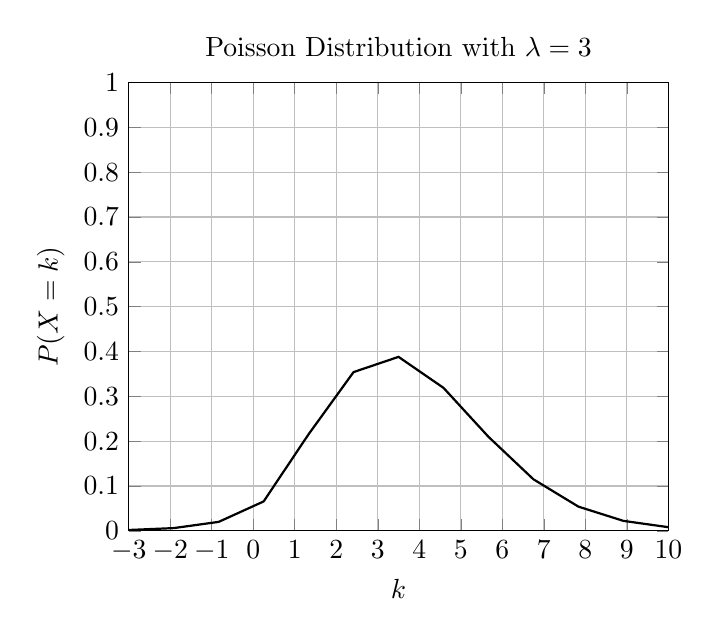
\begin{tikzpicture}
    \begin{axis}
        [title={Poisson Distribution with $\lambda = 3$},
        xlabel={$k$},
        ylabel={$P(X = k)$},
        xmin=-3, xmax=10,
        ymin=0, ymax=1,
        xtick={-3, -2,...,10},
        ytick={0,0.1,...,1},
        grid=major
    ]
    \addplot[domain=-3:10, samples=13, thick]{(3^x * exp(-3)) / (factorial(x))};
    \end{axis}
    \end{tikzpicture}
    \caption{Poisson Distribution with $\lambda = 3$}
\end{figure}
We show that the Poisson distribution is a special case of the Binomial distribution. Consider a Binomial distribution with parameters $n$ (number of trials) and $p$ (probability of success in each trial). The PMF of a Binomial random variable $X$ is given by:
$$P(X = k) = \binom{n}{k} p^k (1 - p)^{n - k}$$
As $n\to \infty, p \to 0, np = \lambda$, we have - 
$$P(X=k) = \frac{(n)(n-1)(n-2)\cdots(n-k+1)}{k!} p^k \frac{(1 - \frac{np}{n})^{n}}{(1-p)^k}$$
$$\implies P(X=k) = \frac{1(1-\frac{1}{n})(1-\frac{2}{n})...(1-\frac{k+1}{n})}{k!}(np)^k\frac{(1 - \frac{np}{n})^n}{(1-p)^k}$$
Since $n\to \infty$, we have $1(1-\frac{1}{n})...(1 - \frac{k+1}{n}) = 1(1)...(1) = 1$. Since $p\to 0$, we have $(1-p)^k = 1$. We further have $np = \lambda$. Then, we have -  
$$P(X=k) = \frac{\lambda^k}{k!}(1-\frac{\lambda}{n})^k = \frac{\lambda^k}{k!}e^{-\lambda}$$
\subsubsection{Moments of the Poisson Distribution}
We can easily obtain the moments of the Poisson Distribution by setting the same limits as we did above. 
Therefore, we have - 
\begin{align*}
    \mu &= np = \lambda \\
    \mu_2 &= np(1-p) = \lambda \\
    \mu_3 &= np(1-p)(1-2p) = \lambda \\
    \mu_4 &= 3n^2p^2(1-p)^2 + np(1-p)(1-6p(1-p)) = 3\lambda^2 + \lambda
\end{align*}
\begin{mytheorem}[Sum of PMF of Poisson Distribution is 1]
    The sum of the probabilities in the probability mass function (PMF) of a Poisson distribution is equal to 1. That is, for a Poisson random variable $X$ with parameter $\lambda$, we have:
    $$\sum_{k=0}^{\infty} P(X = k) = 1$$
    We define $P(X = k)$ as:
    $$P(X = k) = \frac{\lambda^k e^{-\lambda}}{k!}$$
\end{mytheorem}
\begin{proof}
    To show that the sum of the probabilities in the PMF is equal to 1, we sum $P(X = k)$ over all possible values of $k$ from 0 to $\infty$:
    \begin{align*}
        \sum_{k=0}^{\infty} P(X = k) &= \sum_{k=0}^{\infty} \frac{\lambda^k e^{-\lambda}}{k!} \\
        &= e^{-\lambda} \sum_{k=0}^{\infty} \frac{\lambda^k}{k!} \\
        &= e^{-\lambda} e^{\lambda} \quad \text{(by the Taylor series expansion of } e^{\lambda}) \\
        &= 1
    \end{align*}
    Hence proved.
\end{proof}
\section{Joint Distributions}
Here we consider two discrete random variables $X$ and $Y$, and we define their joint distribution. Joint distributions can be used to model the relationship between two random variables, and they are often used in statistical analysis and machine learning. \\
We can define the joint distribution of $X$ and $Y$ using a joint probability mass function (PMF) or a joint probability density function (PDF), depending on whether the random variables are discrete or continuous. The joint PMF or PDF gives the probability or density of each possible combination of values for $X$ and $Y$.
\subsection{Joint PMF and Distributions}
\begin{mydefinition}{Joint Probability Mass Function (PMF)}
    The joint probability mass function (PMF) of two discrete random variables $X$ and $Y$ is a function that gives the probability that $X$ takes on a specific value $x$ and $Y$ takes on a specific value $y$. It is denoted as $P(X = x, Y = y)$ or simply $P(x, y)$. The joint PMF must satisfy the following properties:
    \begin{itemize}
        \item Non-negativity: $P(x, y) \geq 0$ for all possible values of $x$ and $y$.
        \item Normalization: The sum of the joint probabilities over all possible values of $x$ and $y$ must equal 1. That is, $\sum_{x} \sum_{y} P(x, y) = 1$.
        \item Marginalization: The marginal PMFs of $X$ and $Y$ can be obtained by summing the joint PMF over the other variable. That is, $P(X = x) = \sum_{y} P(x, y)$ and $P(Y = y) = \sum_{x} P(x, y)$.
    \end{itemize}
\end{mydefinition}
\begin{example}
    Consider two discrete random variables $X$ and $Y$ that represent the outcome of rolling two fair six-sided dice. The possible values for both $X$ and $Y$ are $\{1, 2, 3, 4, 5, 6\}$. The joint PMF of $X$ and $Y$ can be represented in a table as follows:
    \begin{table}[H]
        \centering
        \begin{tabular}{c|cccccc}
            $P(X = x, Y = y)$ & $Y=1$ & $Y=2$ & $Y=3$ & $Y=4$ & $Y=5$ & $Y=6$ \\
            \hline
            $X=1$ & $\frac{1}{36}$ & $\frac{1}{36}$ & $\frac{1}{36}$ & $\frac{1}{36}$ & $\frac{1}{36}$ & $\frac{1}{36}$ \\
            $X=2$ & $\frac{1}{36}$ & $\frac{1}{36}$ & $\frac{1}{36}$ & $\frac{1}{36}$ & $\frac{1}{36}$ & $\frac{1}{36}$ \\
            $X=3$ & $\frac{1}{36}$ & $\frac{1}{36}$ & $\frac{1}{36}$ & $\frac{1}{36}$ & $\frac{1}{36}$ & $\frac{1}{36}$ \\
            $X=4$ & $\frac{1}{36}$ & $\frac{1}{36}$ & $\frac{1}{36}$ & $\frac{1}{36}$ & $\frac{1}{36}$ & $\frac{1}{36}$ \\
            $X=5$ & $\frac{1}{36}$ & $\frac{1}{36}$ & $\frac{1}{36}$ & $\frac{1}{36}$ & $\frac{1}{36}$ & $\frac{1}{36}$ \\
            $X=6$ & $\frac{1}{36}$ & $\frac{1}{36}$ & $\frac{1}{36}$ & $\frac{1}{36}$ & $\frac{1}{36}$ & $\frac{1}{36}$ \\
        \end{tabular}
    \end{table}
    Each entry in the table represents the probability of a specific combination of outcomes for $X$ and $Y$. For example, the probability of rolling a 1 on the first die and a 2 on the second die is $\frac{1}{36}$. The sum of all probabilities in the table is equal to 1, satisfying the normalization property of the joint PMF. The marginal PMFs can be obtained by summing the joint PMF over the other variable. For example, the marginal PMF of $X$ is given by:
    $$P(X = x) = \sum_{y=1}^{6} P(X = x, Y = y) = \sum_{y=1}^{6} \frac{1}{36} = \frac{6}{36} = \frac{1}{6}$$
    for $x = 1, 2, 3, 4, 5, 6$. Similarly, the marginal PMF of $Y$ is also $\frac{1}{6}$ for $y = 1, 2, 3, 4, 5, 6$.
\end{example} \\
\begin{example}
    Consider the same example of tossing 2 fair coins. Let $X$ be the random variable representing the number of heads obtained in the first coin toss, and let $Y$ be the random variable representing the number of heads obtained in the second coin toss. The possible values for both $X$ and $Y$ are $\{0, 1\}$. The joint PMF of $X$ and $Y$ can be represented in a table as follows:
    \begin{table}[H]
        \centering
        \begin{tabular}{c|cc}
            $P(X = x, Y = y)$ & $Y=0$ & $Y=1$ \\
            \hline
            $X=0$ & $\frac{1}{4}$ & $\frac{1}{4}$ \\
            $X=1$ & $\frac{1}{4}$ & $\frac{1}{4}$ \\
        \end{tabular}
    \end{table}
    Each entry in the table represents the probability of a specific combination of outcomes for $X$ and $Y$. For example, the probability of getting 0 heads in the first toss and 1 head in the second toss is $\frac{1}{4}$. The sum of all probabilities in the table is equal to 1, satisfying the normalization property of the joint PMF. The marginal PMFs can be obtained by summing the joint PMF over the other variable. For example, the marginal PMF of $X$ is given by:
    $$P(X = x) = \sum_{y=0}^{1} P(X = x, Y = y) = \sum_{y=0}^{1} \frac{1}{4} = \frac{2}{4} = \frac{1}{2}$$
    for $x = 0, 1$. Similarly, the marginal PMF of $Y$ is also $\frac{1}{2}$ for $y = 0, 1$.
\end{example}
\subsection{Covariance and Correlation}
\begin{mydefinition}{Covariance}
    The covariance between two random variables $X$ and $Y$ is a measure of how much the two variables change together. It is defined as:
    $$Cov(X, Y) = E[(X - E[X])(Y - E[Y])]$$
    where $E[X]$ and $E[Y]$ are the expected values (means) of $X$ and $Y$, respectively. The covariance can also be expressed in terms of the joint expectation:
    $$Cov(X, Y) = E[XY] - E[X]E[Y]$$
    The covariance can take on any value, positive or negative. A positive covariance indicates that when one variable increases, the other variable tends to increase as well. A negative covariance indicates that when one variable increases, the other variable tends to decrease. A covariance of zero indicates that there is no linear relationship between the two variables.
\end{mydefinition}
\begin{example}
    Consider the example given above, where $X$ and $Y$ represent the outcomes of rolling two fair six-sided dice. The expected values of $X$ and $Y$ are both 3.5. We can calculate the covariance between $X$ and $Y$ as follows:
    \begin{align*}
        E[XY] &= \sum_{x=1}^{6} \sum_{y=1}^{6} xy P(X = x, Y = y) \\
        &= \sum_{x=1}^{6} \sum_{y=1}^{6} xy \cdot \frac{1}{36} \\
        &= \frac{1}{36} \sum_{x=1}^{6} x \sum_{y=1}^{6} y \\
        &= \frac{1}{36} (1 + 2 + 3 + 4 + 5 + 6)(1 + 2 + 3 + 4 + 5 + 6) \\
        &= \frac{1}{36} (21)(21) = \frac{441}{36} = 12.25
    \end{align*}
    Therefore, the covariance between $X$ and $Y$ is:
    $$Cov(X, Y) = E[XY] - E[X]E[Y] = 12.25 - (3.5)(3.5) = 12.25 - 12.25 = 0$$
    This indicates that there is no linear relationship between the outcomes of the two dice rolls.
\end{example}
\begin{mydefinition}{Correlation}
    The correlation between two random variables $X$ and $Y$ is a measure of the strength and direction of the linear relationship between the two variables. It is defined as:
    $$\rho_{X,Y} = \frac{Cov(X, Y)}{\sigma_X \sigma_Y}$$
    where $Cov(X, Y)$ is the covariance between $X$ and $Y$, and $\sigma_X$ and $\sigma_Y$ are the standard deviations of $X$ and $Y$, respectively. 
\end{mydefinition}
\begin{mytheorem}[Range of Correlation Coefficient]
    The correlation coefficient $\rho_{X,Y}$ between two random variables $X$ and $Y$ always lies in the range of -1 to 1. That is, 
    $$-1 \leq \rho_{X,Y} \leq 1$$
\end{mytheorem}
\begin{proof}
By using the Cauchy-Schwarz inequality, we have:
\begin{align*}
    |E[(X - E[X])(Y - E[Y])]|^2 &\leq E[(X - E[X])^2] E[(Y - E[Y])^2] \\
    \implies Cov(X, Y)^2 &\leq Var(X) Var(Y) \\
    \implies \frac{Cov(X, Y)^2}{Var(X) Var(Y)} &\leq 1 \\
    \implies -1 \leq \frac{Cov(X, Y)}{\sqrt{Var(X)} \sqrt{Var(Y)}} &\leq 1 \\
    \implies -1 \leq \rho_{X,Y} &\leq 1
\end{align*}
\end{proof}
\begin{mynote}
    A correlation coefficient of 1 indicates a perfect positive linear relationship between the two variables, meaning that as one variable increases, the other variable also increases in a perfectly linear manner. A correlation coefficient of -1 indicates a perfect negative linear relationship, meaning that as one variable increases, the other variable decreases in a perfectly linear manner. A correlation coefficient of 0 indicates no linear relationship between the two variables. However, it is important to note that a correlation coefficient of 0 does not necessarily imply that there is no relationship between the variables; there may still be a non-linear relationship present.
\end{mynote}
\begin{example}
    Suppose a box has $N$ balls and $A$ of them are white. Let $x$ be the number of draws required to get $r$ white balls without replacement. \\ 
    Let $x_i$ be the number of draws required to get the $i^{th}$ white ball after getting the $(i-1)^{th}$ white ball. Then, the joint distribution of $x_1, x_2, \ldots, x_r$ is given by:
    $$P(x_1 = k_1, x_2 = k_2, \ldots, x_r = k_r) = \frac{\binom{N - A}{k_1 - 1} \binom{N - A - (k_1 - 1)}{k_2 - 1} \cdots \binom{N - A - \sum_{i=1}^{r-1} (k_i - 1)}{k_r - 1}}{\binom{N}{\sum_{i=1}^{r} k_i}}$$
    where $k_i$ is the number of draws required to get the $i^{th}$ white ball after getting the $(i-1)^{th}$ white ball. \\
    The covariance between $x_i$ and $x_j$ for $i \neq j$ can be calculated as:
    $$Cov(x_i, x_j) = \frac{(N - A)(N - A - 1)}{(A + 1)^2 (A + 2)}$$
    The variance of $x_i$ can be calculated as:
    $$Var(x_i) = \frac{(N - A)(N + 1)}{(A + 1)^2 (A + 2)}$$
    Therefore, the correlation coefficient between $x_i$ and $x_j$ for $i\neq j$ is given by:
    $$\rho_{x_i, x_j} = \frac{Cov(x_i, x_j)}{\sqrt{Var(x_i)} \sqrt{Var(x_j)}} = \sqrt{\frac{N - A}{N + 1}}$$
\end{example}
\subsection{Multinomial Distribution}
\begin{mydefinition}{Multinomial Distribution}
    The multinomial distribution is a generalization of the binomial distribution to more than two categories. It describes the probabilities of obtaining a specific combination of counts for each category in a fixed number of independent trials, where each trial can result in one of $k$ possible outcomes. The multinomial distribution is characterized by the following parameters:
    \begin{itemize}
        \item $n$: The total number of independent trials.
        \item $p_1, p_2, \ldots, p_k$: The probabilities of each of the $k$ possible outcomes, where $\sum_{i=1}^{k} p_i = 1$.
    \end{itemize}
    The probability mass function (PMF) of the multinomial distribution is given by:
    $$P(X_1 = x_1, X_2 = x_2, \ldots, X_k = x_k) = \frac{n!}{x_1! x_2! \cdots x_k!} p_1^{x_1} p_2^{x_2} \cdots p_k^{x_k}$$
    where $X_i$ is the random variable representing the count of outcome $i$, and $x_i$ is the observed count for outcome $i$, with the constraint that $\sum_{i=1}^{k} x_i = n$.
\end{mydefinition}
\begin{figure}[H]
\begin{tabular}{c|c}
    \hline
    Parameter & Description \\
    \hline
    $n$ & Total number of independent trials \\
    $k$ & Number of possible outcomes in each trial \\
    $p_i$ & Probability of outcome $i$ occurring in a single trial, where $i = 1, 2, \ldots, k$ and $\sum_{i=1}^{k} p_i = 1$ \\
    $X_i$ & Random variable representing the count of outcome $i$ in $n$ trials \\
    $x_i$ & Observed count for outcome $i$, with the constraint that $\sum_{i=1}^{k} x_i = n$ \\
    \hline
\end{tabular} 
\caption{Parameters of the Multinomial Distribution}
\end{figure}
\begin{mynote}
We can visualize the PMF of the multinomial distribution using a 3D plot, where the x-axis represents the number of trials, the y-axis represents the probability, and the z-axis represents the outcome combinations. Each point in the 3D space corresponds to a specific combination of counts for the $k$ outcomes, and the height of the point represents the probability of that combination occurring. \\
To create such a plot, we can use software tools like Python with libraries such as Matplotlib or Plotly, or mathematical software like MATLAB. The plot will help us understand how the probabilities of different outcome combinations change as we vary the number of trials and the probabilities of each outcome. The resulting 3D surface will provide insights into the behavior of the multinomial distribution and its dependence on the parameters $n$ and $p_i$.
\end{mynote}
\begin{example}
    Consider a scenario where we want to know the probability of 3 distinct outcomes occurring 1 time, 4 times and 5 times respectively in 10 independent trials. Let the probabilities of the three outcomes be $p_1 = 0.2$, $p_2 = 0.5$ and $p_3 = 0.3$. \\
    Here, we have $n = 10$, $k = 3$, $p_1 = 0.2$, $p_2 = 0.5$, $p_3 = 0.3$. The pmf of the multinomial distribution is given by:
    $$P(X_1 = x_1, X_2 = x_2, X_3 = x_3) = \frac{10!}{x_1! x_2! x_3!} (0.2)^{x_1} (0.5)^{x_2} (0.3)^{x_3}$$
    where $x_1 + x_2 + x_3 = 10$. \\
    Using the multinomial distribution, we can calculate the probability as follows:
    \begin{align*}
        P(X_1 = 1, X_2 = 4, X_3 = 5) &= \frac{10!}{1! 4! 5!} (0.2)^1 (0.5)^4 (0.3)^5 \\
        &= \frac{3628800}{1 \cdot 24 \cdot 120} (0.2) (0.0625) (0.00243) \\
        &= 1260 \cdot 0.2 \cdot 0.0625 \cdot 0.00243 \\
        &\approx 0.038
    \end{align*}
    Therefore, the probability of the three outcomes occurring 1 time, 4 times and 5 times respectively in 10 independent trials is approximately 0.038.
    Suppose we want to visualize the PMF of the multinomial distribution for this example. We can create a 3D plot where the x-axis represents the number of trials, the y-axis represents the probability, and the z-axis represents the outcome combinations. Each point in the 3D space corresponds to a specific combination of counts for the three outcomes, and the height of the point represents the probability of that combination occurring.
    \begin{figure}[H]
        \centering 
        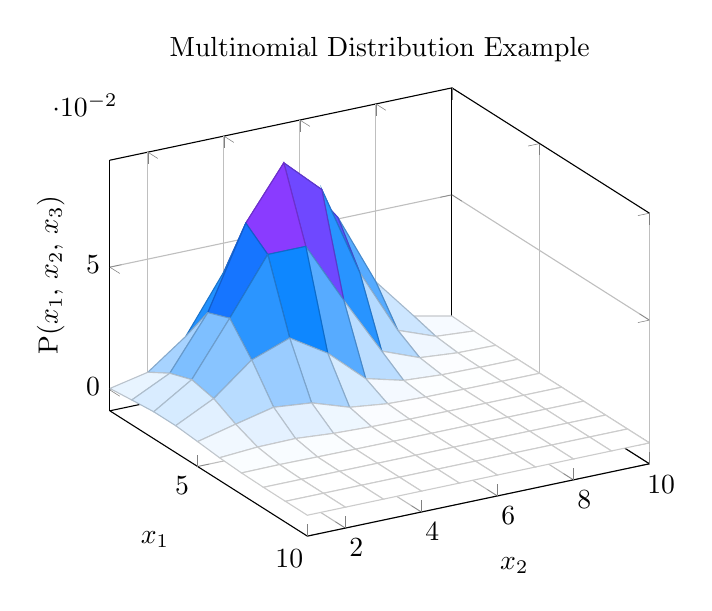
\begin{tikzpicture}
            \begin{axis}[
                xlabel={$x_1$},
                ylabel={$x_2$},
                zlabel={P($x_1$, $x_2$, $x_3$)},
                title={Multinomial Distribution Example},
                grid=major,
                colormap/cool,
                view={60}{30}
            ]
            \addplot3[
                surf,
                domain=1:10,
                y domain=1:10,
                samples=10,
                samples y=10
            ]
            { (10!/(x! * y! * (10 - x - y)!)) * (0.2)^x * (0.5)^y * (0.3)^(10 - x - y) };
            \end{axis}
        \end{tikzpicture}
        \caption{3D Plot of Multinomial Distribution PMF}
    \end{figure}
\end{example}
\subsection{Extraction of Probabilities of Individual Random Variables from Multinomial Distribution}
\begin{mytheorem}[Marginal Distribution of Multinomial Distribution]
    Summing over the other variables in a multinomial distribution gives a Binomial distribution for the variable of interest. Specifically, if $(X_1, X_2, \ldots, X_k)$ follows a multinomial distribution with parameters $n$ and probabilities $p_1, p_2, \ldots, p_k$, then the marginal distribution of $X_1$ is a Binomial distribution with parameters $n$ and $p_1$. That is,
    $$P(X_1 = x_1) = \binom{n}{x_1} p_1^{x_1} (1 - p_1)^{n - x_1}$$
\end{mytheorem}
\begin{proof}
Suppose we want $P(X_1 = x_1)$, but are given a multinomial distribution with parameters $n, p_1, p_2, \ldots, p_k$. We can extract the required probability as follows:
\begin{align*}
    P(X_1 = x_1) &= \sum_{x_2=0}^{n-x_1} \sum_{x_3=0}^{n-x_1-x_2} \ldots \sum_{x_k=0}^{n - x_1 - x_2 - \ldots - x_{k-1}} P(X_1 = x_1, X_2 = x_2, \ldots, X_k = x_k) \\
    &= \sum_{x_2=0}^{n-x_1} \sum_{x_3=0}^{n-x_1-x_2} \ldots \sum_{x_k=0}^{n - x_1 - x_2 - \ldots - x_{k-1}} \frac{n!}{x_1! x_2! \ldots x_k!} p_1^{x_1} p_2^{x_2} \ldots p_k^{x_k} \\
    &= \frac{n!}{x_1! (n - x_1)!} p_1^{x_1} \sum_{x_2=0}^{n-x_1} \sum_{x_3=0}^{n-x_1-x_2} \ldots \sum_{x_k=0}^{n - x_1 - x_2 - \ldots - x_{k-1}} \frac{(n - x_1)!}{x_2! \ldots x_k!} p_2^{x_2} \ldots p_k^{x_k} \\
    &= \frac{n!}{x_1! (n - x_1)!} p_1^{x_1} (p_2 + p_3 + \ldots + p_k)^{n - x_1} \\
    &= \frac{n!}{x_1! (n - x_1)!} p_1^{x_1} (1 - p_1)^{n - x_1}
\end{align*}
This is the PMF of a Binomial distribution with parameters $n$ and $p_1$. Therefore, we have shown that the marginal distribution of $X_1$ in a multinomial distribution is a Binomial distribution with parameters $n$ and $p_1$.
\end{proof}
\begin{mytheorem}[Correlation between Random Variables in Multinomial Distribution]
    In a multinomial distribution with parameters $n$ and probabilities $p_1, p_2, \ldots, p_k$, the correlation coefficient between any two random variables $X_i$ and $X_j$ (for $i \neq j$) is given by:
    $$\rho_{X_i, X_j} = -\sqrt{\frac{p_i p_j}{(1 - p_i)(1 - p_j)}}$$
\end{mytheorem}
\begin{proof}
To find the correlation coefficient between $X_i$ and $X_j$, we first need to calculate the covariance $Cov(X_i, X_j)$ and the variances $Var(X_i)$ and $Var(X_j)$.
\begin{align*}
    E[X_i] &= np_i \\
    E[X_j] &= np_j \\
    Var(X_i) &= np_i(1 - p_i) \\
    Var(X_j) &= np_j(1 - p_j) \\
    E[X_i X_j] &= n(n - 1)p_i p_j \\
    Cov(X_i, X_j) &= E[X_i X_j] - E[X_i]E[X_j] \\
    &= n(n - 1)p_i p_j - (np_i)(np_j) \\
    &= -np_i p_j
\end{align*}
Now, we can calculate the correlation coefficient:
\begin{align*}
    \rho_{X_i, X_j} &= \frac{Cov(X_i, X_j)}{\sqrt{Var(X_i)} \sqrt{Var(X_j)}} \\
    &= \frac{-np_i p_j}{\sqrt{np_i(1 - p_i)} \sqrt{np_j(1 - p_j)}} \\
    &= -\sqrt{\frac{p_i p_j}{(1 - p_i)(1 - p_j)}}
\end{align*}
Hence proved.
\end{proof}
\subsection{Moment Generating Function of Multinomial Distribution}
The moment generating function (MGF) of a multinomial distribution with parameters $n$ and probabilities $p_1, p_2, \ldots, p_k$ is given by:
$$M(t_1, t_2, \ldots, t_k) = \left( p_1 e^{t_1} + p_2 e^{t_2} + \ldots + p_k e^{t_k} \right)^n$$
where $t_1, t_2, \ldots, t_k$ are the variables corresponding to the random variables $X_1, X_2, \ldots, X_k$. The MGF can be used to derive the moments of the distribution by taking partial derivatives with respect to the variables $t_i$ and evaluating them at $t_i = 0$ for all $i$. \\
Let us derive the first moment (mean) of the random variable $X_i$ using the MGF:
\begin{align*}
    E[X_i] &= \frac{\partial M(t_1, t_2, \ldots, t_k)}{\partial t_i} \bigg|_{t_1=0, t_2=0, \ldots, t_k=0} \\
    &= n p_i \left( p_1 + p_2 + \ldots + p_k \right)^{n-1} \\
    &= n p_i
\end{align*}
Similarly, we can derive the second moment (variance) of the random variable $X_i$:
\begin{align*}
    E[X_i^2] &= \frac{\partial^2 M(t_1, t_2, \ldots, t_k)}{\partial t_i^2} \bigg|_{t_1=0, t_2=0, \ldots, t_k=0} \\
    &= n p_i (1 - p_i) + (n p_i)^2 \\
    Var(X_i) &= E[X_i^2] - (E[X_i])^2 \\
    &= n p_i (1 - p_i)
\end{align*}
\begin{exercise}
    Let $X_1, X_2, \ldots, X_k$ be k independent poisson random variables with parameters $\lambda_1, \lambda_2, \ldots, \lambda_k$ respectively. Show that the joint distribution of $X_1, X_2, \ldots, X_k$ is a multinomial distribution with parameters $n = \sum_{i=1}^{k} X_i$ and probabilities $p_i = \frac{\lambda_i}{\sum_{j=1}^{k} \lambda_j}$ for $i = 1, 2, \ldots, k$.
\end{exercise}
\begin{proof}
    We want to show that the joint distribution of $X_1, X_2, \ldots, X_k$ is a multinomial distribution with parameters $n = \sum_{i=1}^{k} X_i$ and probabilities $p_i = \frac{\lambda_i}{\sum_{j=1}^{k} \lambda_j}$ for $i = 1, 2, \ldots, k$. \\
    The joint PMF of $X_1, X_2, \ldots, X_k$ is given by:
    \begin{align*}
        P(X_1 = x_1, X_2 = x_2, \ldots, X_k = x_k) &= \prod_{i=1}^{k} P(X_i = x_i) \\
        &= \prod_{i=1}^{k} \frac{e^{-\lambda_i} \lambda_i^{x_i}}{x_i!} \\
        &= e^{-\sum_{i=1}^{k} \lambda_i} \prod_{i=1}^{k} \frac{\lambda_i^{x_i}}{x_i!}
    \end{align*}
    Now, we can rewrite the above expression as:
    \begin{align*}
        P(X_1 = x_1, X_2 = x_2, \ldots, X_k = x_k) &= e^{-\sum_{i=1}^{k} \lambda_i} \frac{(\sum_{i=1}^{k} \lambda_i)^{\sum_{i=1}^{k} x_i}}{\prod_{i=1}^{k} x_i!} \prod_{i=1}^{k} \left( \frac{\lambda_i}{\sum_{j=1}^{k} \lambda_j} \right)^{x_i} \\
        &= e^{-\sum_{i=1}^{k} \lambda_i} \frac{(\sum_{i=1}^{k} \lambda_i)^{n}}{\prod_{i=1}^{k} x_i!} p_1^{x_1} p_2^{x_2} \ldots p_k^{x_k}
    \end{align*}
    where $n = \sum_{i=1}^{k} x_i$ and $p_i = \frac{\lambda_i}{\sum_{j=1}^{k} \lambda_j}$ for $i = 1, 2, \ldots, k$. \\
    This is the PMF of a multinomial distribution with parameters $n$ and probabilities $p_1, p_2, \ldots, p_k$. Therefore, we have shown that the joint distribution of $X_1, X_2, \ldots, X_k$ is a multinomial distribution with the specified parameters.
\end{proof}
\subsection{Expectation and Variance}
\begin{mytheorem}[Algebra of Expectation and Variance]
    Let $X$ and $Y$ be two discrete random variables. Then - 
    \begin{itemize}
        \item $E(aX + bY) = aE(X) + bE(Y)$ if $E(X), E(Y) < \infty$.
        \item $Var(aX + bY) = a^2 Var(X) + b^2 Var(Y) + 2ab Cov(X, Y)$ if $Var(X), Var(Y) < \infty$.
    \end{itemize}
\end{mytheorem}
\begin{proof}
    We prove the two parts of the theorem separately. \\ 
        \textbf{Part 1:} We want to show that $E(aX + bY) = aE(X) + bE(Y)$ if $E(X), E(Y) < \infty$. 
        \begin{align*}
            E(aX + bY) &= \sum_i \sum_j (ai + bj) P(X=i, Y=j) \\
            &= a \sum_i \sum_j i P(X=i, Y=j) + b \sum_i \sum_j j P(X=i, Y=j) \\
            &= aE(X) + bE(Y)
        \end{align*}
        \textbf{Part 2:} We want to show that $Var(aX + bY) = a^2 Var(X) + b^2 Var(Y) + 2ab Cov(X, Y)$ if $Var(X), Var(Y) < \infty$. 
        \begin{align*}
            Var(aX + bY) &= E((aX + bY)^2) - (E(aX + bY))^2 \\
            &= E(a^2X^2 + 2abXY + b^2Y^2) - (aE(X) + bE(Y))^2 \\
            &= a^2E(X^2) + 2abE(XY) + b^2E(Y^2) - (a^2(E(X))^2 + 2abE(X)E(Y) + b^2(E(Y))^2) \\
            &= a^2(E(X^2) - (E(X))^2) + b^2(E(Y^2) - (E(Y))^2) + 2ab(E(XY) - E(X)E(Y)) \\
            &= a^2 Var(X) + b^2 Var(Y) + 2ab Cov(X, Y)
        \end{align*}
\end{proof}
\begin{mydefinition}{Conditional Expectation and Variance}
    The conditional expectation of a random variable $X$ given another random variable $Y$ is defined as:
    $$E(X|Y=y) = \sum_i i P(X=i|Y=y)$$
    where $P(X=i|Y=y)$ is the conditional probability of $X$ given $Y$. The conditional variance of $X$ given $Y$ is defined as:
    $$Var(X|Y=y) = E((X - E(X|Y=y))^2|Y=y) = E(X^2|Y=y) - (E(X|Y=y))^2$$
\end{mydefinition}
\begin{mytheorem}[Conditional Expectation and Variance]
    Let $X$ and $Y$ be two discrete random variables. Then - 
    \begin{itemize}
        \item $E(X) - E(E(X|Y))$ if $E(X) < \infty$.
        \item $Var(X) = E(Var(X|Y)) + Var(E(X|Y))$ if $Var(E(X|Y)) < \infty$.    
    \end{itemize}
\end{mytheorem}
\begin{proof}
    We prove the two parts of the theorem separately. \\ 
        \textbf{Part 1:} We want to show that $E(X) = E(E(X|Y))$ if $E(X) < \infty$. 
        \begin{align*}
            E(X) &= \sum_i \sum_j iP(X=i, Y=j) \\
            &= \sum_i \sum_j iP(X=i|Y=j)P(Y=j) \\
            &= \sum_j P(Y=j) \sum_i iP(X=i|Y=j) \\
            &= \sum_j P(Y=j) E(X|Y=j) \\
            &= E_Y(E_X(X|Y)) \\
        \end{align*}
        \textbf{Part 2:} We want to show that $Var(X) = E(Var(X|Y)) + Var(E(X|Y))$ if $Var(E(X|Y)) < \infty$. 
        \begin{align*}
            E(Var(X|Y)) + Var(E(X|Y)) &= E(E(X^2|Y) - (E(X|Y))^2) + E((E(X|Y))^2) - (E(E(X|Y)))^2 \\
            &= E(E(X^2|Y)) - (E(E(X|Y)))^2 \\
            &= E(X^2) - (E(X))^2 \\
            &= Var(X)
        \end{align*}
\end{proof}
\subsection{Mode and Median of Binomial Distribution}
We define the mode and median of a Binomial distribution.
\begin{mydefinition}{Mode and Median of Binomial Distribution}
    The mode of a Binomial distribution with parameters $n$ and $p$ is the value of $k$ that maximizes the probability mass function (PMF) of the distribution. The PMF of a Binomial random variable $X$ is given by:
    $$P(X = k) = \binom{n}{k} p^k (1 - p)^{n - k}$$
    for $k = 0, 1, 2, \ldots, n$. The mode can be found by taking the derivative of the PMF with respect to $k$, setting it to zero, and solving for $k$. The mode is given by:
    $$\text{Mode} = \lfloor (n + 1)p \rfloor$$
    if $(n + 1)p$ is not an integer, and both $\lfloor (n + 1)p \rfloor$ and $\lfloor (n + 1)p \rfloor - 1$ are modes if $(n + 1)p$ is an integer. \\
    The median of a Binomial distribution is the value of $m$ such that:
    $$P(X \leq m) \geq 0.5 \quad \text{and} \quad P(X \geq m) \geq 0.5$$
\end{mydefinition}
Let $X$ be a random variable following a Binomial distribution with parameters $n$ and $p$. The mean of $X$ is given by:
$$\mu = E(X) = np$$
To find the mode of $X$, we need to find the value $m$ such that $P(X = m)$ is maximized.
Let $f(k) = P(X = k) = \binom{n}{k} p^k (1 - p)^{n - k}$ be the PMF of $X$. Let us consider - 
\begin{align*}
    \frac{f(k+1)}{f(k)} &= \frac{\binom{n}{k+1} p^{k+1} (1 - p)^{n - (k + 1)}}{\binom{n}{k} p^k (1 - p)^{n - k}} \\
    &= \frac{(n-k)p}{(k+1)(1-p)} = m \\
    \implies f(k+1) &= \frac{(n-k)p}{(k+1)(1-p)}f(k) = mf(k) \\ 
\end{align*}
Finally let us consider - 
\begin{align*}
    \frac{f(k)}{f(k-1)} &= \frac{\binom{n}{k} p^k (1 - p)^{n - k}}{\binom{n}{k-1} p^{k-1} (1 - p)^{n - (k - 1)}} \\
    &= \frac{(n-k+1)p}{k(1-p)} = m
\end{align*}
Then we have - 
\begin{align*}
    \frac{(n-k)p}{(k+1)(1-p)} \lesseqgtr 1 &\iff (n-k)p \lesseqgtr (k+1)(1-p) \\
    &\iff np - kp \lesseqgtr k + 1 - kp - p \\
    &\iff np - 1 + p \lesseqgtr k \\
    &\iff (n+1)p - 1 \lesseqgtr k \\
    \frac{(n-k+1)p}{k(1-p)} \lesseqgtr 1 &\iff (n-k+1)p \lesseqgtr k(1-p) \\
\end{align*}
We have two cases - 
\begin{enumerate}
    \item If $(n+1)p - 1$ is a fraction, then for $k > (n+1)p - 1$, we have $f(k) < f(k-1)$ and for $k < (n+1)p - 1$, we have $f(k) > f(k-1)$. Therefore we have - 
    $$f(0) < f(1) < ... < f(m) > f(m+1) > ... > f(n)$$
    Therefore, the mode is $m = \lfloor (n+1)p - 1 \rfloor + 1 = \lfloor (n+1)p \rfloor$.
    \item If $(n+1)p - 1$ is an integer, then for $k \geq (n+1)p - 1$, we have $$k \lesseqgtr (n+1)p - 1 \implies f(k+1) \gtreqless f(k)$$. Then, we have - 
    $$f(0) < f(1) < ... < f(m) = f(m) > f((n+1)p + 1) > ... > f(n)$$
    Therefore, the modes are $m$ and $m+1$. 
\end{enumerate}
\begin{example}
    Consider a Binomial distribution with parameters $n = 10$ and $p = 0.3$. The mean of the distribution is given by:
    $$\mu = E(X) = np = 10 \cdot 0.3 = 3$$
    To find the mode of the distribution, we calculate $(n + 1)p$:
    $$(n + 1)p = (10 + 1) \cdot 0.3 = 11 \cdot 0.3 = 3.3$$
    Since $(n + 1)p$ is not an integer, we take the floor of this value to find the mode:
    $$\text{Mode} = \lfloor (n + 1)p \rfloor = \lfloor 3.3 \rfloor = 3$$
    Therefore, the mode of the Binomial distribution with parameters $n = 10$ and $p = 0.3$ is 3.
    We have the pmf of the distribution as follows -
    \begin{table}[H]
        \centering
        \begin{tabular}{c|ccccccccccc}
            $k$ & 0 & 1 & 2 & 3 & 4 & 5 & 6 & 7 & 8 & 9 & 10 \\
            \hline
            $P(X = k)$ & $0.0282$ & $0.1211$ & $0.2335$ & $0.2668$ & $0.2001$ & $0.1029$ & $0.0368$ & $0.0090$ & $0.0014$ & $0.0001$ & $0.0000$ \\
        \end{tabular}
    \end{table}
    The PMF has a distinct peak at $k = 3$, which is the mode of the distribution.
    \begin{figure}[H]
        \centering
        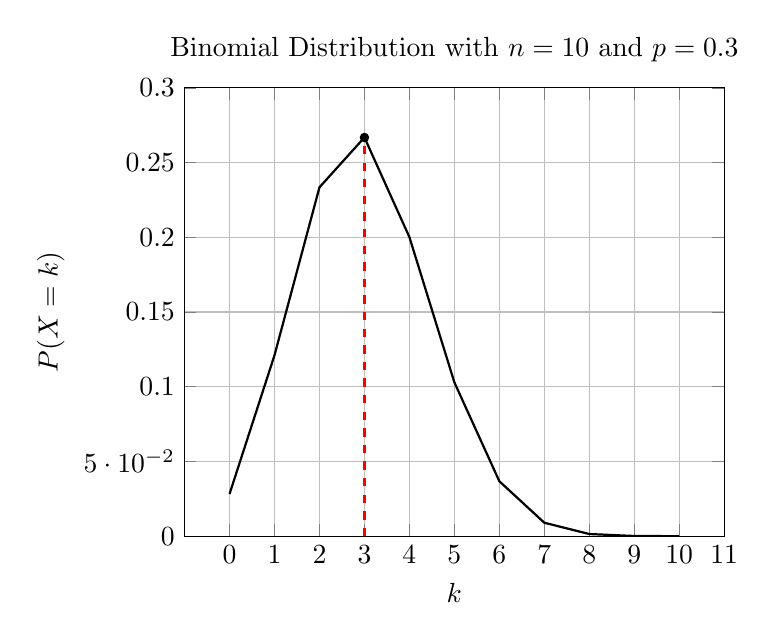
\begin{tikzpicture}
        \begin{axis}
            [title={Binomial Distribution with $n = 10$ and $p = 0.3$},
            xlabel={$k$},
            ylabel={$P(X = k)$},
            xmin=-1, xmax=11,
            ymin=0, ymax=0.3,
            xtick={0,...,11},
            ytick={0,0.05,...,0.3},
            grid=major
        ]
        \addplot[domain=0:10, samples=11, thick]{((10!)/(x! * (10-x)!)) * (0.3)^x * (0.7)^(10-x)};
        \addplot[only marks, mark=*, mark size=1.5pt] coordinates {(3, 0.2668)};
        \addplot[line width=1pt, color=red, dashed] coordinates {(3,0) (3,0.2668)};
        \end{axis}
        \end{tikzpicture}
        \caption{Binomial Distribution with $n = 10$ and $p = 0.3$, mode at $k = 3$}
    \end{figure}
\end{example}
\subsection{Bimodal Distribution}
We define a bimodal distribution. Bimodal distributions can arise in various contexts, such as in the analysis of data with two distinct groups or populations, or in the study of physical phenomena with two dominant modes of behavior.
\begin{mydefinition}{Bimodal Distribution}
    A bimodal distribution is a probability distribution that has two distinct modes, or peaks, in its probability density function (PDF) or probability mass function (PMF). This means that there are two values of the random variable that occur with higher frequency than other values. Bimodal distributions can be either continuous or discrete, and they can arise in various contexts, such as in the analysis of data with two distinct groups or populations, or in the study of physical phenomena with two dominant modes of behavior. \\
    We denote the modes of a bimodal distribution as $m_1$ and $m_2$, where $m_1 + 1 = m_2$.
\end{mydefinition}
\begin{example}
    Consider a random variable $X$ that follows a Binomial distribution with parameters $n = 9$ and $p = 0.5$. The PMF of $X$ is given by:
    $$P(X = k) = \binom{9}{k} (0.5)^k (0.5)^{9 - k}$$
    for $k = 0, 1, 2, \ldots, 9$. The PMF of $X$ can be calculated as follows:
    \begin{table}[H]
        \centering
        \begin{tabular}{c|cccccccccc}
            $k$ & 0 & 1 & 2 & 3 & 4 & 5 & 6 & 7 & 8 & 9 \\
            \hline
            $P(X = k)$ & $\frac{1}{512}$ & $\frac{9}{512}$ & $\frac{36}{512}$ & $\frac{84}{512}$ & $\frac{126}{512}$ & $\frac{126}{512}$ & $\frac{84}{512}$ & $\frac{36}{512}$ & $\frac{9}{512}$ & $\frac{1}{512}$ \\
        \end{tabular}
    \end{table}
    The PMF has two distinct peaks at $k = 4$ and $k = 5$, which are the modes of the distribution. Therefore, the Binomial distribution with parameters $n = 9$ and $p = 0.5$ is a bimodal distribution with modes at $m_1 = 4$ and $m_2 = 5$.
    \begin{figure}[H]
        \centering
        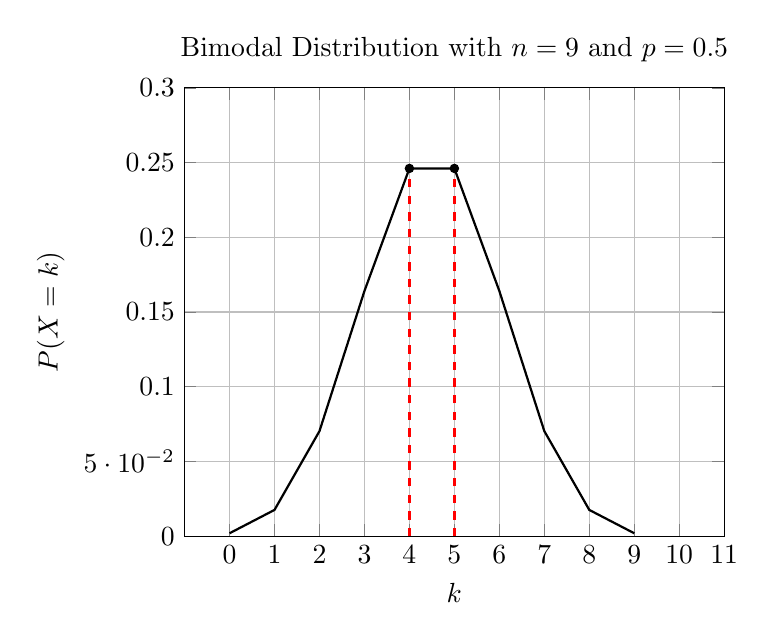
\begin{tikzpicture}
        \begin{axis}
            [title={Bimodal Distribution with $n = 9$ and $p = 0.5$},
            xlabel={$k$},
            ylabel={$P(X = k)$},
            xmin=-1, xmax=11,
            ymin=0, ymax=0.3,
            xtick={0,...,11},
            ytick={0,0.05,...,0.3},
            grid=major
        ]
        \addplot[domain=0:9, samples=10, thick]{((9!)/(x! * (9-x)!)) * (0.5)^x * (0.5)^(9-x)};
        \addplot[only marks, mark=*, mark size=1.5pt] coordinates {(4, 0.2461) (5, 0.2461)};
        \addplot[line width=1pt, color=red, dashed] coordinates {(4,0) (4,0.2461)};
        \addplot[line width=1pt, color=red, dashed] coordinates {(5,0) (5,0.2461)};
        \end{axis}
        \end{tikzpicture}
        \caption{Bimodal Distribution with $n = 10$ and $p = 0.5$}
    \end{figure}
\end{example}
\subsection{Mode of Poisson Distribution}
Let $X$ be a random variable following a Poisson distribution with parameter $\lambda$. Let us denote the pmf of $X$ as $f(k) = P(X = k) = \frac{\lambda^k e^{-\lambda}}{k!}$ for $k = 0, 1, 2, \ldots$. We want to find the mode of the distribution. \\
Let us consider -
\begin{align*}
    \frac{f(k+1)}{f(k)} &= \frac{\frac{\lambda^{k+1} e^{-\lambda}}{(k+1)!}}{\frac{\lambda^k e^{-\lambda}}{k!}} \\
    &= \frac{\lambda}{k+1} = m \\
    \implies f(k+1) &= \frac{\lambda}{k+1} f(k) = mf(k) \\
\end{align*}
Then, we have - 
\begin{align*}
    \frac{f(k+1)}{f(k)} \lesseqgtr 1 &\iff \frac{\lambda}{k+1} \lesseqgtr 1 \\
    &\iff \lambda \lesseqgtr k + 1 \\
    &\iff \lambda - 1 \lesseqgtr k \\
\end{align*}
We have two cases -
\begin{enumerate}
    \item If $\lambda - 1$ is a fraction, then for $k > \lambda - 1$, we have $f(k) < f(k-1)$ and for $k < \lambda - 1$, we have $f(k) > f(k-1)$. Therefore we have - 
    $$f(0) < f(1) < ... < f(m) > f(m+1) > ...$$
    Therefore, the mode is $m = \lfloor \lambda - 1 \rfloor + 1 = \lfloor \lambda \rfloor$.
    \item If $\lambda - 1$ is an integer, then for $k \geq \lambda - 1$, we have $$k \lesseqgtr \lambda - 1 \implies f(k+1) \gtreqless f(k)$$ 
    Then, we have - 
    $$f(0) < f(1) < ... < f(m) = f(m) > f((\lambda - 1) + 1) > ...$$
    Therefore, the modes are $m$ and $m+1$.
\end{enumerate}
\begin{example}
    Let us consider a Poisson distribution with parameter $\lambda = 4.5$. This is a unimodal distribution, since the value of $\lambda - 1$ is not an integer. Unimodal distributions have a single mode. The pmf of the distribution is given by:
    $$P(X = k) = \frac{4.5^k e^{-4.5}}{k!}$$
    for $k = 0, 1, 2, \ldots$. To find the mode of the distribution, we calculate $\lambda - 1$:
    $$\lambda - 1 = 4.5 - 1 = 3.5$$
    Since $\lambda - 1$ is not an integer, we take the floor of this value to find the mode:
    $$\text{Mode} = \lfloor \lambda - 1 \rfloor + 1 = \lfloor 3.5 \rfloor + 1 = 3 + 1 = 4$$
    Therefore, the mode of the Poisson distribution with parameter $\lambda = 4.5$ is 4.
    \begin{table}[H]
        \centering
        \begin{tabular}{c|ccccccccccc}
            $k$ & 0 & 1 & 2 & 3 & 4 & 5 & 6 & 7 & 8 & 9 & 10 \\
            \hline
            $P(X = k)$ & $0.0111$ & $0.0499$ & $0.1123$ & $0.1685$ & $0.1896$ & $0.1706$ & $0.1279$ & $0.0824$ & $0.0464$ & $0.0232$ & $0.0104$ \\
        \end{tabular}
        \caption{PMF of Poisson Distribution with $\lambda = 4.5$, mode at $k = 4$}
    \end{table}
    \begin{figure}[H]
        \centering
        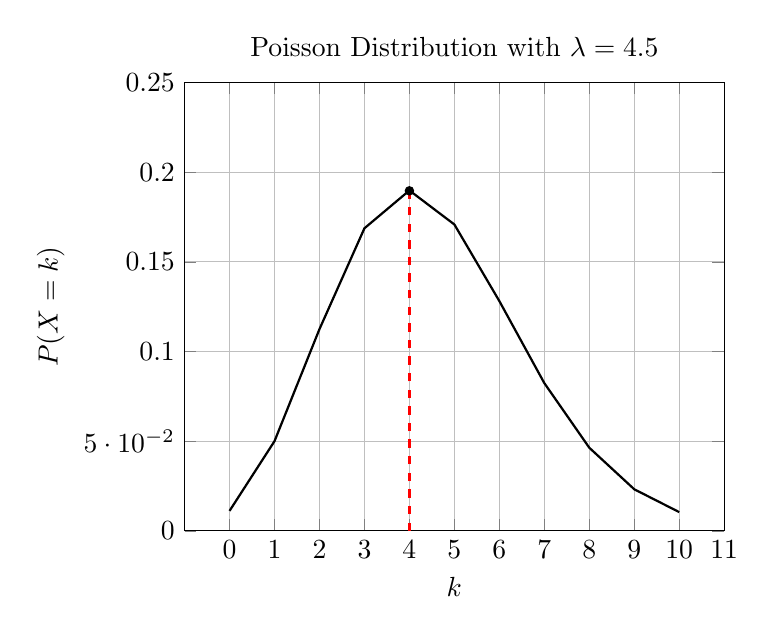
\begin{tikzpicture}
        \begin{axis}
            [title={Poisson Distribution with $\lambda = 4.5$},
            xlabel={$k$},
            ylabel={$P(X = k)$},
            xmin=-1, xmax=11,
            ymin=0, ymax=0.25,
            xtick={0,...,11},
            ytick={0,0.05,...,0.25},
            grid=major
        ]
        \addplot[domain=0:10, samples=11, thick]{(4.5^x * exp(-4.5)) / (factorial(x))};
        \addplot[only marks, mark=*, mark size=1.5pt] coordinates {(4, 0.1896)};
        \addplot[line width=1pt, color=red, dashed] coordinates {(4,0) (4,0.1896)};
        \end{axis}
        \end{tikzpicture}
        \caption{Poisson Distribution with $\lambda = 4.5$, mode at $k = 4$}
    \end{figure}
The figure above shows the PMF of the Poisson distribution with parameter $\lambda = 4.5$. The PMF has a distinct peak at $k = 4$, which is the mode of the distribution. Such a distribution is called a unimodal distribution, and these arise when the parameter $\lambda$ is not an integer.
\end{example}
\begin{mynote}
    We can similarly derive the mode of any discrete distribution by considering the ratio of the pmf at consecutive points and analyzing its behavior. The mode can be found by identifying the point where the pmf transitions from increasing to decreasing, which corresponds to the maximum value of the pmf. \\ An example of a bimodal distribution is the Poisson distribution when the parameter $\lambda$ is an integer. In this case, the modes of the distribution are given by $m$ and $m+1$, where $m = \lambda - 1$.
\end{mynote}
\begin{example}
    Here we consider an example of a bimodal Poisson distribution. We know that a bimodal Poisson distribution occurs when the parameter $\lambda$ is an integer. In this case, the modes of the distribution are given by $m$ and $m+1$, where $m = \lambda - 1$. \\
    Let us consider a Poisson distribution with parameter $\lambda = 5$. The pmf of the distribution is given by:
    $$P(X = k) = \frac{5^k e^{-5}}{k!}$$
    for $k = 0, 1, 2, \ldots$. To find the mode of the distribution, we calculate $\lambda - 1$:
    $$\lambda - 1 = 5 - 1 = 4$$
    Since $\lambda - 1$ is an integer, we have two modes:
    $$\text{Modes} = \{m, m+1\} = \{4, 5\}$$
    Therefore, the modes of the Poisson distribution with parameter $\lambda = 5$ are 4 and 5.
    \begin{table}[H]
        \centering
        \begin{tabular}{c|ccccccccccc}
            $k$ & 0 & 1 & 2 & 3 & 4 & 5 & 6 & 7 & 8 & 9 & 10 \\
            \hline
            $P(X = k)$ & $0.0067$ & $0.0337$ & $0.0842$ & $0.1404$ & $0.1755$ & $0.1755$ & $0.1463$ & $0.1045$ & $0.0653$ & $0.0363$ & $0.0182$ \\
        \end{tabular}
        \caption{PMF of Poisson Distribution with $\lambda = 5$, modes at $k = 4$ and $k = 5$}
    \end{table}
    \begin{figure}[H]
        \centering
        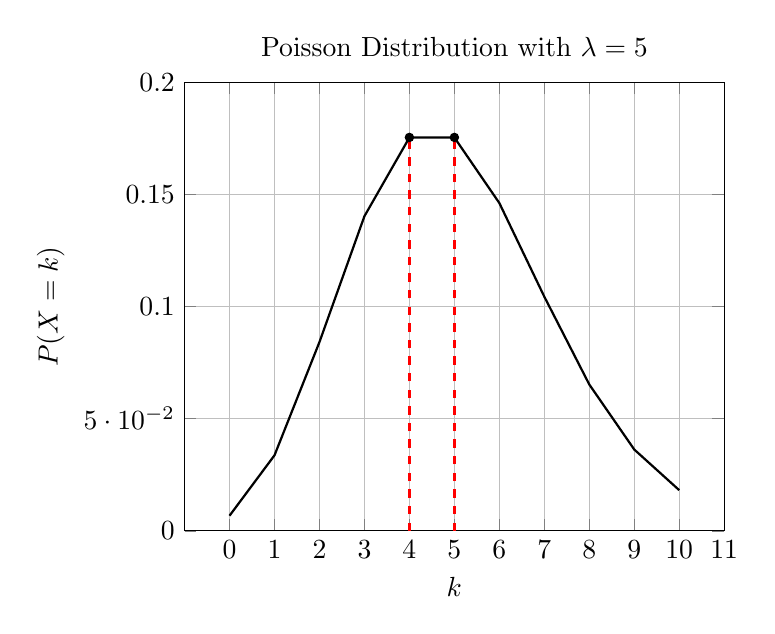
\begin{tikzpicture}
        \begin{axis}
            [title={Poisson Distribution with $\lambda = 5$},
            xlabel={$k$},
            ylabel={$P(X = k)$},
            xmin=-1, xmax=11,
            ymin=0, ymax=0.2,
            xtick={0,...,11},
            ytick={0,0.05,...,0.2},
            grid=major
        ]
        \addplot[domain=0:10, samples=11, thick]{(5^x * exp(-5)) / (factorial(x))};
        \addplot[only marks, mark=*, mark size=1.5pt] coordinates {(4, 0.1755) (5, 0.1755)};
        \addplot[line width=1pt, color=red, dashed] coordinates {(4,0) (4,0.1755)};
        \addplot[line width=1pt, color=red, dashed] coordinates {(5,0) (5,0.1755)};
        \end{axis}
        \end{tikzpicture}
        \caption{Poisson Distribution with $\lambda = 5$, modes at $k = 4$ and $k = 5$}
    \end{figure}
\end{example}
\begin{mynote}
    Properties of the Mode:
    \begin{itemize}
        \item The mode is the value that appears most frequently in a data set or distribution.
        \item A distribution can have one mode (unimodal), two modes (bimodal), or more (multimodal).
        \item The mode is not affected by extreme values (outliers) in the data set.
        \item In a symmetric distribution, the mode, mean, and median are all equal.
        \item In a skewed distribution, the mode is typically less than the mean and median in a right-skewed distribution, and greater than the mean and median in a left-skewed distribution.
        \item The mode can be used to identify the most common category or value in categorical data.
        \item The mode is particularly useful for nominal data, where the mean and median cannot be defined.
    \end{itemize}
\end{mynote}
\section{Geometric Distribution}
\subsection{Definition and Properties}
A geometric distribution is a discrete probability distribution that models the number of trials needed to achieve the first success in a sequence of independent Bernoulli trials, where each trial has the same probability of success. We encounter geometric distributions in various real-world scenarios, such as quality control, reliability testing, and customer service.
\begin{mydefinition}{Geometric Distribution}
    A random variable $X$ is said to follow a geometric distribution with parameter $p$ if its probability mass function (PMF) is given by:
    $$P(X = k) = (1 - p)^{k} p$$
    for $k = 1, 2, 3, \ldots$, where $0 < p < 1$ is the probability of success on each trial. \\ 
    This is called a geometric distributions since this generates a geometric series when we sum over all possible values of $k$.
\end{mydefinition}
\begin{example}
    Consider a scenario where we are rolling a fair six-sided die and we want to find the probability of rolling a 3 for the first time on the 4th roll. Here, rolling a 3 is considered a success, and rolling any other number is considered a failure. The probability of success on each roll is $p = \frac{1}{6}$, and the probability of failure is $1 - p = \frac{5}{6}$. \\
    Let $X$ be the random variable representing the number of rolls needed to get the first 3. Then, $X$ follows a geometric distribution with parameter $p = \frac{1}{6}$. We want to find $P(X = 4)$, which is the probability of getting the first 3 on the 4th roll. Using the PMF of the geometric distribution, we have:
    \begin{align*}
        P(X = 4) &= (1 - p)^{4 - 1} p \\
        &= \left(\frac{5}{6}\right)^{3} \cdot \frac{1}{6} \\
        &= \frac{125}{1296} \approx 0.09645
    \end{align*}
    Therefore, the probability of rolling a 3 for the first time on the 4th roll is approximately $0.09645$ or $9.645\%$.
    We have the pmf of the distribution as follows -
    \begin{table}[H]
        \centering
        \begin{tabular}{c|cccccccccc}
            $k$ & 1 & 2 & 3 & 4 & 5 & 6 & 7 & 8 & 9 & 10 \\
            \hline
            $P(X = k)$ & $0.1667$ & $0.1389$ & $0.1157$ & $0.0965$ & $0.0804$ & $0.0670$ & $0.0558$ & $0.0465$ & $0.0388$ & $0.0323$ \\
        \end{tabular}
        \caption{PMF of Geometric Distribution with $p = \frac{1}{6}$}
    \end{table}
    \begin{figure}[H]
        \centering
        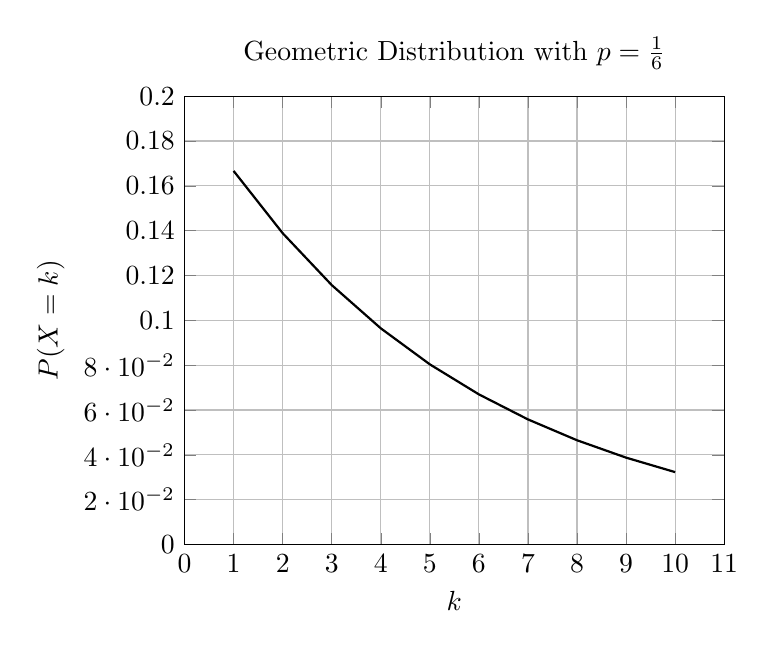
\begin{tikzpicture}
        \begin{axis}
            [title={Geometric Distribution with $p = \frac{1}{6}$},
            xlabel={$k$},
            ylabel={$P(X = k)$},
            xmin=0, xmax=11,
            ymin=0, ymax=0.2,
            xtick={0,...,11},
            ytick={0,0.02,...,0.2},
            grid=major
        ]
        \addplot[domain=1:10, samples=10, thick]{(5/6)^(x-1) * (1/6)};
        \end{axis}
        \end{tikzpicture}
        \caption{Geometric Distribution with $p = \frac{1}{6}$}
    \end{figure}
\end{example}
\begin{mynote}
    The geometric distribution is the only discrete distribution that has the memoryless property. This means that the probability of success on the next trial is independent of the number of previous failures. In other words, the probability of success on the next trial is always $p$, regardless of how many trials have been conducted so far without success. \\\\
    Mathematically, the memoryless property can be expressed as:
    $$P(X > m + n | X > m) = P(X > n)$$
    for all non-negative integers $m$ and $n$. This property is unique to the geometric distribution among discrete distributions. \\ 
    The memoryless property has important implications in various applications, such as in queuing theory, reliability engineering, and survival analysis. It allows us to simplify calculations and make predictions about future events based on past observations.
\end{mynote}
\begin{mytheorem}{Mean of Geometric Distribution}
    Let $X$ be a random variable following a geometric distribution with parameter $p$. Then, the mean of $X$ is given by:
    $$E(X) = \frac{1-p}{p}$$
\end{mytheorem}
\begin{proof}
    We want to show that $E(X) = \frac{1}{p}$.
    \begin{align*}
        E(X) &= \sum_{k=1}^{\infty} k P(X = k) \\
        &= \sum_{k=1}^{\infty} k (1 - p)^{k} p \\
        &= p \sum_{k=1}^{\infty} k (1 - p)^{k} \\
        &= p \cdot \frac{1 - p}{(1 - (1 - p))^2} \quad \text{(using the formula for the sum of a geometric series)} \\
        &= p \cdot \frac{1 - p}{p^2} = \frac{1 - p}{p}
    \end{align*}
\end{proof}
\begin{mytheorem}[Sum of PMF of Geometric Distribution]
    Let $X$ be a random variable following a geometric distribution with parameter $p$. Then, the sum of the pmf of $X$ over all possible values of $k$ is equal to 1, i.e.,
    $$\sum_{k=1}^{\infty} P(X = k) = 1$$
\end{mytheorem}
\begin{proof}
    We want to show that $\sum_{k=1}^{\infty} P(X = k) = 1$.
    \begin{align*}
        \sum_{k=1}^{\infty} P(X = k) &= \sum_{k=1}^{\infty} (1 - p)^{k} p \\
        &= p \sum_{k=1}^{\infty} (1 - p)^{k} \\
        &= p \cdot \frac{1}{1 - (1 - p)} \quad \text{(using the formula for the sum of a geometric series)} \\
        &= p \cdot \frac{1}{p} = 1
    \end{align*}
\end{proof}
\section{Negative Binomial Distribution}
\subsection{Definition and Properties}
Let $X =$ Number of failures before the $k^th$ success. Then, we have the following pmf -
$$P(X = x) = \binom{x+k-1}{k-1} p^k (1-p)^x \quad x = 0, 1, 2, \ldots$$
This is called the Negative Binomial Distribution.
\begin{mydefinition}{Negative Binomial Distribution}
    A random variable $X$ is said to follow a Negative Binomial distribution with parameters $k$ and $p$ if its probability mass function (PMF) is given by:
    $$P(X = x) = \binom{x+k-1}{k-1} p^k (1-p)^x$$
    for $x = 0, 1, 2, \ldots$, where $0 < p < 1$ is the probability of success on each trial and $k$ is the number of successes. \\
    The Negative Binomial distribution models the number of failures before the $k^{th}$ success in a sequence of independent Bernoulli trials.
\end{mydefinition}
Let us simplify the pmf of the Negative Binomial distribution. We have -
\begin{align*}
    P(X = x) &= \binom{x+k-1}{k-1} p^k (1-p)^x \\
    &= \frac{(x+k-1)!}{(k-1)! x!} p^k (1-p)^x \\
    &= \frac{(x+k-1)(x+k-2) \ldots k}{x!} p^k (1-p)^x \\
    &= \frac{k(k+1)(k+2) \ldots (x+k-1)}{x!} p^k (1-p)^x \\
    &= \frac{-k(-k-1)(-k-2) \ldots (-k-(x-1))}{x!} p^k (1-p)^x \\
    &= \binom{-k}{x} (-1)^x p^k (1-p)^x \\
\end{align*}
Now let $p = \frac{1}{Q}$, then we have $1 - p = q = \frac{P}{Q}$. We have: \\
$1 + P = 1 + qQ = 1 + (1 - p) \cdot \frac{1}{p} = \frac{1}{p} = Q$. \\
Therefore, we have -
\begin{align*}
    P(X = x) &= \binom{-k}{x} (-1)^x p^k (1-p)^x \\
    &= \binom{-k}{x} (-1)^x \left(\frac{1}{Q}\right)^k \left(\frac{P}{Q}\right)^x \\
    &= \binom{-k}{x} (-1)^x \frac{P^x}{Q^{k+x}} \\
\end{align*}
This is the pmf of the Negative Binomial distribution in terms of $P$ and $Q$. \\
\begin{example}
    Let us consider a scenario where we are conducting a series of independent Bernoulli trials with a success probability of $p = 0.4$. We want to find the probability of having exactly 3 failures before achieving the 2nd success. Here, the number of successes $k = 2$ and the number of failures $x = 3$. \\
    Let $X$ be the random variable representing the number of failures before the 2nd success. Then, $X$ follows a Negative Binomial distribution with parameters $k = 2$ and $p = 0.4$. We want to find $P(X = 3)$, which is the probability of having exactly 3 failures before achieving the 2nd success. Using the PMF of the Negative Binomial distribution, we have:
    \begin{align*}
        P(X = 3) &= \binom{3+2-1}{2-1} (0.4)^2 (1-0.4)^3 \\
        &= \binom{4}{1} (0.4)^2 (0.6)^3 \\
        &= 4 \cdot 0.16 \cdot 0.216 = 0.13824
    \end{align*}
    Therefore, the probability of having exactly 3 failures before achieving the 2nd success is approximately $0.13824$ or $13.824\%$.
    We have the pmf of the distribution as follows -
    \begin{table}[H]
        \centering
        \begin{tabular}{c|cccccccccc}
            $x$ & 0 & 1 & 2 & 3 & 4 & 5 & 6 & 7 & 8 & 9 \\
            \hline
            $P(X = x)$ & $0.16$ & $0.192$ & $0.2304$ & $0.13824$ & $0.10368$ & $0.07776$ & $0.05832$ & $0.04374$ & $0.03281$ & $0.02458$ \\
        \end{tabular}
        \caption{PMF of Negative Binomial Distribution with $k = 2$ and $p = 0.4$}
    \end{table}
    \begin{figure}[H]
        \centering
        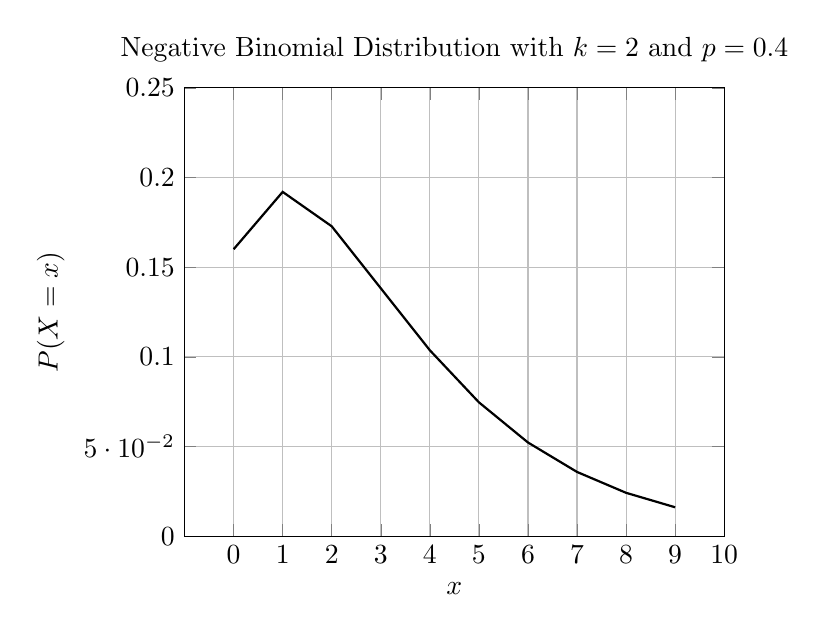
\begin{tikzpicture}
        \begin{axis}
            [title={Negative Binomial Distribution with $k = 2$ and $p = 0.4$},
            xlabel={$x$},
            ylabel={$P(X = x)$},
            xmin=-1, xmax=10,
            ymin=0, ymax=0.25,
            xtick={0,...,10},
            ytick={0,0.05,...,0.25},
            grid=major
        ]
        \addplot[domain=0:9, samples=10, thick]{(factorial(x+2-1)/(factorial(2-1)*factorial(x))) * (0.4)^2 * (0.6)^x};
        \end{axis}
        \end{tikzpicture}
        \caption{Negative Binomial Distribution with $k = 2$ and $p = 0.4$}
    \end{figure}
\end{example}
\section{Hypergeometric Distribution}
\subsection{Definition and Properties}
A hypergeometric distribution is a discrete probability distribution that describes the probability of drawing a specific number of successes in a sample drawn without replacement from a finite population containing a fixed number of successes and failures. It is commonly used in scenarios where the population size is small, and the sampling is done without replacement, such as quality control, card games, and lottery draws.
\begin{mydefinition}{Hypergeometric Distribution}
    A random variable $X$ is said to follow a hypergeometric distribution with parameters $N$, $K$, and $n$ if its probability mass function (PMF) is given by:
    $$P(X = k) = \frac{\binom{K}{k} \binom{N-K}{n-k}}{\binom{N}{n}}$$
    for $k = 0, 1, 2, \ldots, \min(K, n)$, where:
    \begin{itemize}
        \item $N$ is the total number of items in the population,
        \item $K$ is the total number of successes in the population,
        \item $n$ is the number of items drawn from the population,
        \item $k$ is the number of observed successes in the drawn sample.
    \end{itemize}
\end{mydefinition}
\begin{example}
    Consider a scenario where we have a deck of 52 playing cards, which contains 4 aces (successes) and 48 non-aces (failures). We want to find the probability of drawing exactly 2 aces when we randomly select 5 cards from the deck without replacement. \\
    Let $X$ be the random variable representing the number of aces drawn. Then, $X$ follows a hypergeometric distribution with parameters $N = 52$, $K = 4$, and $n = 5$. We want to find $P(X = 2)$, which is the probability of drawing exactly 2 aces. Using the PMF of the hypergeometric distribution, we have:
    \begin{align*}
        P(X = 2) &= \frac{\binom{4}{2} \binom{48}{3}}{\binom{52}{5}} \\
        &= \frac{6 \cdot 17296}{2598960} \\
        &= \frac{103776}{2598960} \approx 0.0399
    \end{align*}
    Therefore, the probability of drawing exactly 2 aces when selecting 5 cards from a standard deck is approximately $0.0399$ or $3.99\%$.
    We have the pmf of the distribution as follows -
    \begin{table}[H]
        \centering
        \begin{tabular}{c|cccccc}
            $k$ & 0 & 1 & 2 & 3 & 4 \\
            \hline
            $P(X = k)$ & $0.6588$ & $0.2995$ & $0.0399$ & $0.0017$ & $0.0001$ \\
        \end{tabular}
        \caption{PMF of Hypergeometric Distribution with $N = 52$, $K = 4$, and $n = 5$}
    \end{table}
    \begin{figure}[H]
        \centering
        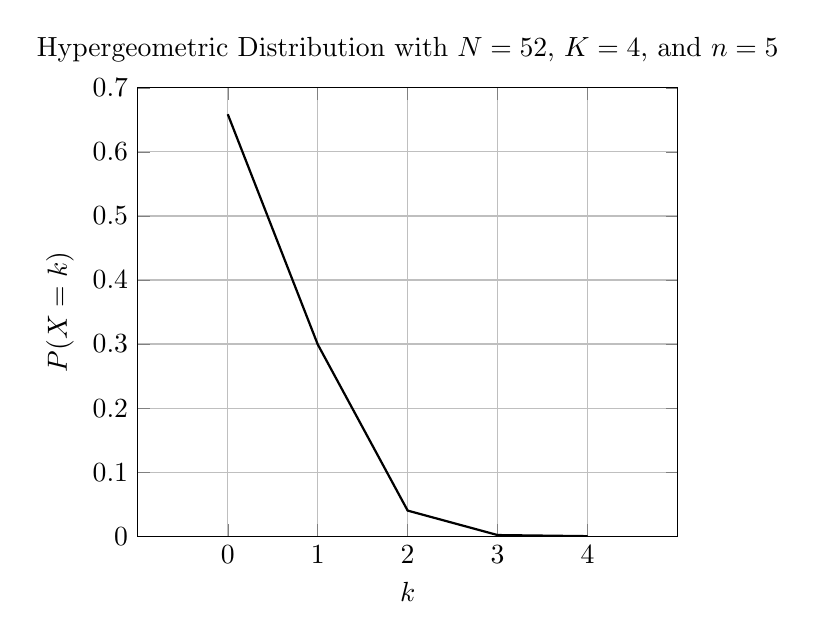
\begin{tikzpicture}
        \begin{axis}
            [title={Hypergeometric Distribution with $N = 52$, $K = 4$, and $n = 5$},
            xlabel={$k$},
            ylabel={$P(X = k)$},
            xmin=-1, xmax=5,
            ymin=0, ymax=0.7,
            xtick={0,...,4},
            ytick={0,0.1,...,0.7},
            grid=major
        ]
        \addplot[domain=0:4, samples=5, thick]{( (factorial(4)/(factorial(x)*factorial(4-x))) * (factorial(48)/(factorial(5-x)*factorial(48-(5-x)))) ) / (factorial(52)/(factorial(5)*factorial(52-5))) };
        \end{axis}
        \end{tikzpicture}
        \caption{Hypergeometric Distribution with $N = 52$, $K = 4$, and $n = 5$}
    \end{figure}
\end{example}






\part{Statsistics}
\chapter{Basic Concepts}
\section{Introduction}
\begin{mydefinition}{Data and Dataset}
    \underemphasise{Data} refers to a collection of facts, figures, or observations that are gathered for analysis, interpretation, or reference. Data can be quantitative (numerical) or qualitative (categorical) in nature and can be collected through various methods such as surveys, experiments, observations, or measurements. In statistics, data is often organized into datasets or databases for further analysis to extract meaningful insights and make informed decisions. \\
    We can represent data numerically by coding qualitative data into numerical values, such as assigning numbers to categories or using binary coding (0 and 1) to represent the presence or absence of a characteristic. \\
    A \underemphasise{dataset} is a structured collection of data that is organized in a specific format, typically in rows and columns. Each row represents an individual observation or record, while each column represents a specific variable or attribute of the data. Datasets can be small or large, depending on the amount of data collected, and can be stored in various formats such as spreadsheets, databases, or text files. Datasets are commonly used in statistical analysis to explore relationships between variables, identify patterns, and make predictions based on the data.
\end{mydefinition}
\begin{example}
    Consider a dataset representing the ages of a group of individuals: [25, 30, 35, 40, 45, 50, 55, 60]. This dataset contains quantitative data, as the ages are numerical values. Each age represents an individual observation in the dataset. \\
    We can organize this data into a structured format as follows:
    \begin{table}[H]
        \centering
        \begin{tabular}{|c|c|}
            \hline
            \textbf{Individual} & \textbf{Age} \\
            \hline
            1 & 25 \\
            2 & 30 \\
            3 & 35 \\
            4 & 40 \\
            5 & 45 \\
            6 & 50 \\
            7 & 55 \\
            8 & 60 \\
            \hline
        \end{tabular}
        \caption{Dataset of Ages}
    \end{table}
    In this table, each row represents an individual observation (the age of each person), and the column represents the variable (age). This structured dataset can be used for further statistical analysis to explore patterns and relationships within the data.
\end{example}
We have two types of data - 
\begin{enumerate}
    \item \underemphasise{Primary Data}
    \begin{itemize}
        \item Data collected for a specificied purpose from the field of inquiry.
        \item It is original data collected directly by the researcher or organization conducting the study.
        \item You need time, effort and resources to collect primary data.
        \item The accuracy and reliability of primary data can be ensured since the researcher has control over the data collection process.
    \end{itemize}
    \item \underemphasise{Secondary Data}
    \begin{itemize}
        \item Data collected for some other purpose but used for a different purpose. Someone else collected the data for their own specified purpose (their primary data), but you are using it for your own purpose (your secondary data).
        \item It is not original data, but rather data that has been previously collected and made available for use by others.
        \item It is generally easier and less expensive to obtain secondary data compared to primary data, as it has already been collected and is readily available for analysis. 
        \item The accuracy and reliability of secondary data may vary depending on the source and quality of the data, as the researcher has no control over the data collection process.
    \end{itemize}
\end{enumerate}

\begin{mydefinition}{Measure}
    A measure is a quantitative value or statistic that is used to describe or summarize a particular aspect of a dataset or population. Measures can be used to analyze various characteristics of data, such as central tendency, dispersion, shape, and relationships between variables. Common measures in statistics include mean, median, mode, variance, standard deviation, range, and percentiles. Measures are essential tools for understanding and interpreting data, as they provide insights into the underlying patterns and trends within the dataset. \\
    Measure theoretically, a measure is a function that assigns a non-negative real number to subsets of a given set, satisfying certain properties such as countable additivity and non-negativity. In statistics, measures are often used to quantify various aspects of data distributions and to make comparisons between different datasets or populations. A measure is defined on a sigma-algebra of subsets of a given set, which allows for the measurement of complex sets and events.
    \begin{mydefinition}{$\sigma$-algebra}
        A $\sigma$-algebra is a collection of subsets of a given set that satisfies certain properties, allowing for the measurement of complex sets and events. Specifically, a $\sigma$-algebra must satisfy the following properties:
        \begin{itemize}
            \item It contains the empty set.
            \item It is closed under complementation, meaning that if a set is in the $\sigma$-algebra, its complement is also in the $\sigma$-algebra.
            \item It is closed under countable unions, meaning that if a countable collection of sets is in the $\sigma$-algebra, their union is also in the $\sigma$-algebra.
        \end{itemize}
        The concept of a $\sigma$-algebra is fundamental in measure theory and probability theory, as it provides a framework for defining measures and probabilities on complex sets and events.
    \end{mydefinition}
\end{mydefinition}
\begin{example}
    Consider a dataset representing the ages of a group of individuals: [25, 30, 35, 40, 45, 50, 55, 60]. We can analyze this dataset using various measures to understand its characteristics. \\
    For example, we can calculate the mean (average) age of the group:
    $$\text{Mean} = \frac{25 + 30 + 35 + 40 + 45 + 50 + 55 + 60}{8} = \frac{340}{8} = 42.5$$
    We can also determine the median (middle value) of the dataset:
    Since there are 8 values, the median is the average of the 4th and 5th values:
    $$\text{Median} = \frac{40 + 45}{2} = \frac{85}{2} = 42.5$$
    Additionally, we can find the mode (most frequently occurring value) of the dataset. In this case, there is no mode since all ages occur only once. \\
    These measures provide insights into the central tendency of the dataset, helping us understand the typical age of individuals in the group.
\end{example}
\section{Data Visualization}
\begin{mydefinition}
{Data Visualization}
    Data visualization is the graphical representation of data and information using visual elements such as charts, graphs, maps, and diagrams. It is a powerful tool for communicating complex data in a clear and concise manner, allowing for easier interpretation and analysis. Data visualization helps to identify patterns, trends, and outliers in the data, making it easier to draw insights and make informed decisions. Common types of data visualizations include bar charts, line graphs, pie charts, scatter plots, histograms, and heatmaps. Effective data visualization requires careful consideration of design principles, such as choosing appropriate chart types, using color effectively, and ensuring clarity and simplicity in the presentation of information.
\end{mydefinition}
Various diagrams and graphs are used in statistics to visually represent data and facilitate understanding of its characteristics. Some common types of diagrams and graphs include:
\begin{itemize}
    \item \underemphasise{Bar Chart}: A bar chart is a graphical representation of categorical data using rectangular bars, where the length of each bar is proportional to the frequency or count of the category it represents. Bar charts are useful for comparing the frequencies of different categories and identifying patterns in the data.
    \item \underemphasise{Histogram}: A histogram is a graphical representation of continuous data that displays the distribution of a dataset by dividing it into intervals (bins) and plotting the frequency or count of data points within each interval. Histograms are useful for visualizing the shape, spread, and central tendency of a dataset.
    \item \underemphasise{Pie Chart}: A pie chart is a circular graph that represents categorical data as slices of a pie, where each slice corresponds to a category and its size is proportional to the frequency or percentage of that category. Pie charts are useful for showing the relative proportions of different categories within a whole.
    \item \underemphasise{Line Graph}: A line graph is a graphical representation of data points connected by straight lines, typically used to show trends or changes over time. Line graphs are useful for visualizing relationships between variables and identifying patterns in time series data.
    \item \underemphasise{Scatter Plot}: A scatter plot is a graphical representation of two continuous variables, where each point represents an observation in the dataset. Scatter plots are useful for visualizing relationships between variables, identifying correlations, and detecting outliers.
\end{itemize}
\subsection{Line Diagrams}
Line diagrams, also known as line graphs, are a type of data visualization that uses lines to connect data points on a graph. They are commonly used to represent trends or changes over time, making them particularly useful for time series data. Line diagrams can help identify patterns, fluctuations, and relationships between variables. \\
\begin{example}
\underemphasise{Modelling Population Growth} - Suppose we have the following data representing the population of a city over a period of years:
\begin{table}[H]
    \centering
    \begin{tabular}{|c|c|}
        \hline
        \textbf{Year} & \textbf{Population} \\
        \hline
        2000 & 500,000 \\
        2005 & 550,000 \\
        2010 & 600,000 \\
        2015 & 650,000 \\
        2020 & 700,000 \\
        \hline
    \end{tabular}
    \caption{Population Data Over Years}
\end{table}
We can create a line diagram to visualize the population growth over the years. \\
\begin{figure}[H]
    \centering
    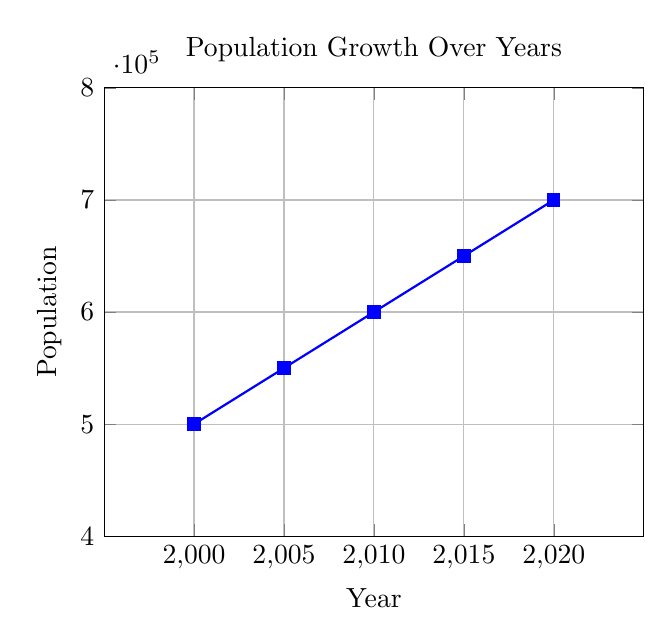
\begin{tikzpicture}
    \begin{axis}
        [title={Population Growth Over Years},
        xlabel={Year},
        ylabel={Population},
        xmin=1995, xmax=2025,
        ymin=400000, ymax=800000,
        xtick={2000, 2005, 2010, 2015, 2020},
        ytick={400000, 500000, 600000, 700000, 800000},
        grid=major
    ]
    \addplot[color=blue, mark=square*, thick] coordinates {
        (2000, 500000)
        (2005, 550000)
        (2010, 600000)
        (2015, 650000)
        (2020, 700000)
    };
    \end{axis}
    \end{tikzpicture}
    \caption{Line Diagram of Population Growth}
\end{figure}
\end{example}
\begin{example}
\underemphasise{Tracking Sales Over Time} - Consider a dataset representing the monthly sales of a company over a year:
\begin{table}[H]
    \centering
    \begin{tabular}{|c|c|}
        \hline
        \textbf{Month} & \textbf{Sales (in \$)} \\
        \hline
        January & 10,000 \\
        February & 12,000 \\
        March & 15,000 \\
        April & 14,000 \\
        May & 18,000 \\
        June & 20,000 \\
        July & 22,000 \\
        August & 21,000 \\
        September & 19,000 \\
        October & 23,000 \\
        November & 25,000 \\
        December & 30,000 \\
        \hline
    \end{tabular}
    \caption{Monthly Sales Data}
\end{table}
We can create a line diagram to visualize the sales trend over the months. \\
\begin{figure}[H]
    \centering
    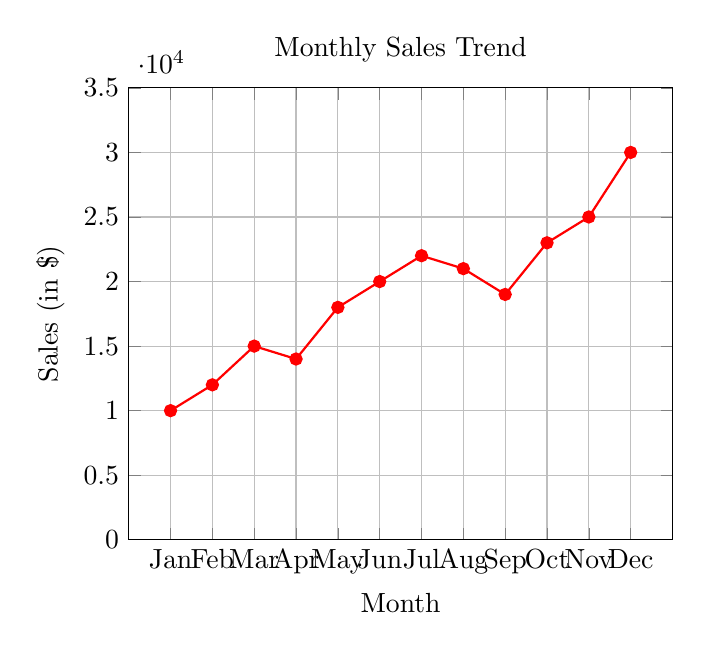
\begin{tikzpicture}
    \begin{axis}
        [title={Monthly Sales Trend},
        xlabel={Month},
        ylabel={Sales (in \$)},
        xmin=0, xmax=13,
        ymin=0, ymax=35000,
        xtick={1,2,3,4,5,6,7,8,9,10,11,12},
        xticklabels={Jan, Feb, Mar, Apr, May, Jun, Jul, Aug, Sep, Oct, Nov, Dec},
        ytick={0,5000,...,35000},
        grid=major,
        width = 0.7\textwidth
    ]
    \addplot[mark = *, color=red, thick] coordinates {
        (1, 10000)
        (2, 12000)
        (3, 15000)
        (4, 14000)
        (5, 18000)
        (6, 20000)
        (7, 22000)
        (8, 21000)
        (9, 19000)
        (10, 23000)
        (11, 25000)
        (12, 30000)
    };
    \end{axis}
    \end{tikzpicture}
    \caption{Line Diagram of Monthly Sales Trend}
\end{figure}
\end{example}
We can see from the above examples that line diagrams are effective in visualizing trends and changes over time, making them a valuable tool for data analysis and interpretation. \\ 
We often encounter multiple line diagrams in a single graph to compare different datasets or variables over the same time period. This allows us to analyze relationships and patterns between the variables more effectively. A specific use case of multiple line diagrams is when we want to compare the sales trends of different products over the same time period, or how stocks of different companies perform over time.
\subsection{Bar Diagrams}
Bar diagrams, also known as bar charts, are a type of data visualization that uses rectangular bars to represent categorical data. The length or height of each bar is proportional to the frequency or count of the category it represents. Bar diagrams are useful for comparing the frequencies of different categories and identifying patterns in the data. \\
\begin{example}
\underemphasise{Comparing Sales of Different Products} - Suppose we have the following data representing the sales of different products in a store:
\begin{table}[H]
    \centering
    \begin{tabular}{|c|c|}
        \hline
        \textbf{Product} & \textbf{Sales (in units)} \\
        \hline
        Product A & 150 \\
        Product B & 200 \\
        Product C & 100 \\
        Product D & 250 \\
        Product E & 300 \\
        \hline
    \end{tabular}
    \caption{Sales Data of Different Products}
\end{table}
We can create a bar diagram to visualize the sales of different products. \\
\begin{figure}[H]
    \centering
    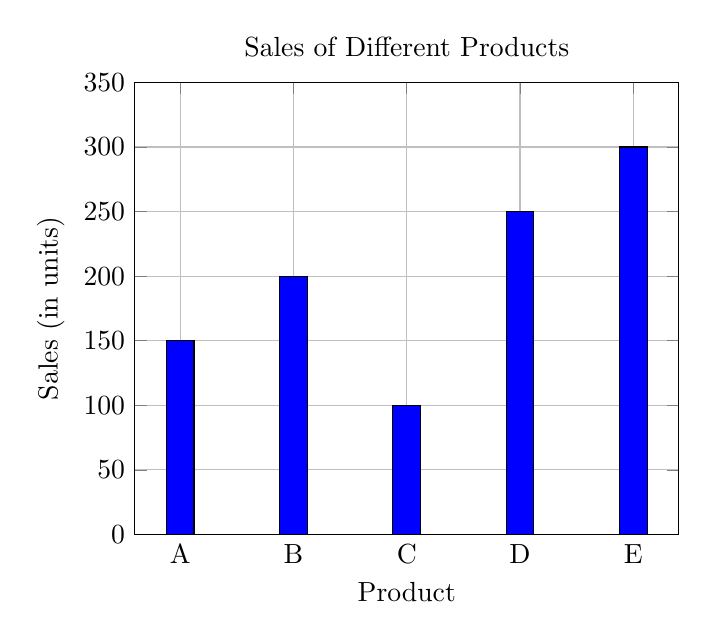
\begin{tikzpicture}
    \begin{axis}
        [title={Sales of Different Products},
        xlabel={Product},
        ylabel={Sales (in units)},
        ymin=0, ymax=350,
        xtick={1,2,3,4,5},
        xticklabels={A, B, C, D, E},
        ytick={0,50,...,350},
        grid=major,
        width = 0.7\textwidth
    ]
    \addplot[ybar, fill=blue] coordinates {
        (1, 150)
        (2, 200)
        (3, 100)
        (4, 250)
        (5, 300)
    };
    \end{axis}
    \end{tikzpicture}
    \caption{Bar Diagram of Sales of Different Products}
\end{figure}
\end{example}
We can see from the above example that bar diagrams are effective in visualizing categorical data and comparing the frequencies of different categories. \\
We often encounter grouped bar diagrams in a single graph to compare multiple datasets or variables across the same categories. This allows us to analyze relationships and patterns between the variables more effectively. A specific use case of grouped bar diagrams is when we want to compare the sales of different products across different regions or time periods.
\subsection{Multiple Bar Diagrams}
Multiple bar diagrams, also known as grouped bar charts, are a type of data visualization that uses multiple rectangular bars to represent different datasets or variables across the same categories. Each group of bars corresponds to a specific category, and each bar within the group represents a different dataset or variable. Multiple bar diagrams are useful for comparing the frequencies of different datasets across the same categories and identifying patterns in the data. \\
\begin{example}
\underemphasise{Comparing Sales of Different Products Across Regions} - Suppose we have the following data representing the sales of different products in two regions:
\begin{table}[H]
    \centering
    \begin{tabular}{|c|c|c|}
        \hline
        \textbf{Product} & \textbf{Region 1 Sales (in units)} & \textbf{Region 2 Sales (in units)} \\
        \hline
        Product A & 150 & 180 \\
        Product B & 200 & 220 \\
        Product C & 100 & 130 \\
        Product D & 250 & 270 \\
        Product E & 300 & 320 \\
        \hline
    \end{tabular}
    \caption{Sales Data of Different Products Across Regions}
\end{table}
We can create a multiple bar diagram to visualize the sales of different products across the two regions. \\
\begin{figure}[H]
    \centering
    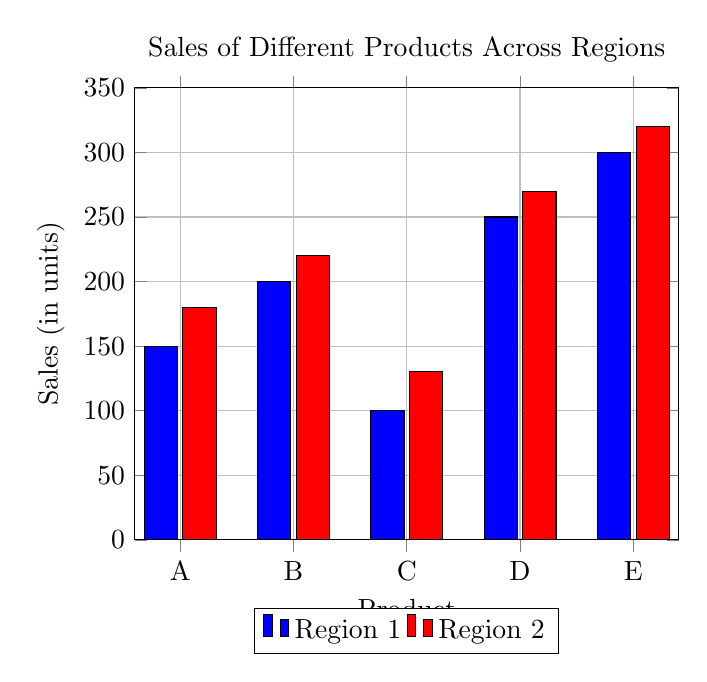
\begin{tikzpicture}
    \begin{axis}
        [title={Sales of Different Products Across Regions},
        ybar,
        xlabel={Product},
        ylabel={Sales (in units)},
        ymin=0, ymax=350,
        xtick={1,2,3,4,5},
        xticklabels={A, B, C, D, E},
        ytick={0,50,...,350},
        grid=major,
        width = 0.7\textwidth,
        bar width=12pt,
        legend style={at={(0.5,-0.15)}, anchor=north, legend columns=-1},
    ]
    \addplot[ybar, fill=blue] coordinates {
        (1, 150)
        (2, 200)
        (3, 100)
        (4, 250)
        (5, 300)
    };
    \addplot[ybar, fill=red] coordinates {
        (1, 180)
        (2, 220)  
        (3, 130)
        (4, 270)
        (5, 320)
    };
    \legend{Region 1, Region 2}
    \end{axis}
    \end{tikzpicture}
    \caption{Multiple Bar Diagram of Sales of Different Products Across Regions}
\end{figure}
\end{example}
We can see from the above example that multiple bar diagrams are effective in visualizing and comparing multiple datasets across the same categories. \\
They allow us to analyze relationships and patterns between the variables more effectively, making them a valuable tool for data analysis and interpretation. We encounter multiple bar diagrams in various fields, such as business, marketing, and social sciences, to compare different datasets and make informed decisions based on the data.
\begin{mynote}
    When creating multiple bar diagrams, it is important to consider the following design principles to ensure clarity and effectiveness:
    \begin{itemize}
        \item Use distinct colors or patterns for each dataset to differentiate between them easily.
        \item Ensure that the bars within each group are spaced appropriately to avoid clutter and improve readability.
        \item Label the axes clearly, including units of measurement, to provide context for the data being presented.
        \item Include a legend to identify each dataset represented in the diagram.
        \item Avoid using too many datasets in a single diagram, as this can lead to confusion and make it difficult to interpret the data.
    \end{itemize}
\end{mynote}
\subsection{Pie Charts}
Pie charts are a type of data visualization that represents categorical data as slices of a pie, where each slice corresponds to a category and its size is proportional to the frequency or percentage of that category. Pie charts are useful for showing the relative proportions of different categories within a whole. \\
\begin{example}
\underemphasise{Visualizing Market Share of Different Companies} - Suppose we have the following data representing the market share of different companies in a specific industry:
\begin{table}[H]
    \centering
    \begin{tabular}{|c|c|}
        \hline
        \textbf{Company} & \textbf{Market Share (in \%)} \\
        \hline
        Company A & 30 \\
        Company B & 25 \\
        Company C & 20 \\
        Company D & 15 \\
        Company E & 10 \\
        \hline
    \end{tabular}
    \caption{Market Share Data of Different Companies}
\end{table}
We can create a pie chart to visualize the market share of different companies. \\
\begin{figure}[H]
    \centering
    \begin{tikzpicture}
    \pie[radius=3, text=legend, explode=0.1]{
        30/Company A,
        25/Company B,
        20/Company C,
        15/Company D,
        10/Company E
    }
    \end{tikzpicture}
    \caption{Pie Chart of Market Share of Different Companies}
\end{figure}
\end{example}
We can see from the above example that pie charts are effective in visualizing the relative proportions of different categories within a whole. We encounter pie charts in various fields, such as business, marketing, and social sciences, to represent categorical data and make informed decisions based on the data. 
\subsection{Scatter Plots and Heat Maps}
Scatter plots and heat maps are two types of data visualization techniques used to represent relationships between variables and patterns in data. \\
A scatter plot is a graphical representation of two continuous variables, where each point represents an observation in the dataset. Scatter plots are useful for visualizing relationships between variables, identifying correlations, and detecting outliers. \\
A heat map is a graphical representation of data where individual values are represented as colors in a matrix. Heat maps are useful for visualizing patterns and trends in large datasets, as well as identifying areas of high or low intensity. \\
\begin{example}
We use scatter plots to visualize the relationship between two variables. It is especially useful for a large dataset with many data points. It also helps to identify correlations and outliers in the data. \\
Lets consider a dataset representing the relationship between hours studied and exam scores of each student in a class of 40 students. We will not put the actual data here, but we can create a scatter plot to visualize the relationship between the two variables. \\
\begin{figure}[H]
    \centering
    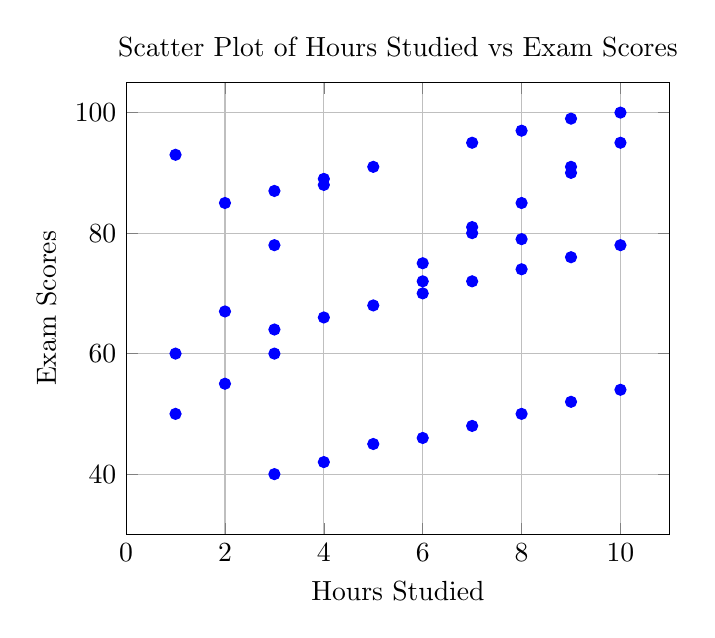
\begin{tikzpicture}
    \begin{axis}
        [title={Scatter Plot of Hours Studied vs Exam Scores},
        xlabel={Hours Studied},
        ylabel={Exam Scores},
        xmin=0, xmax=11,
        ymin=30, ymax=105,
        grid=major,
        width = 0.7\textwidth
    ]
    \addplot[only marks, mark=*, color=blue] coordinates {
        (1, 50)
        (2, 55)
        (3, 60)
        (6, 75)
        (7, 80)
        (8, 85)
        (9, 90)
        (10, 95)
        (1, 93)
        (2, 67)
        (3, 78)
        (4, 88)
        (5, 45)
        (6, 72)
        (7, 81)
        (8, 79)
        (9, 91)
        (1, 60)
        (3, 64)
        (4, 66)
        (5, 68)
        (6, 70)
        (7, 72)
        (8, 74)
        (9, 76)
        (10, 78)
        (2, 85)
        (3, 87)
        (4, 89)
        (5, 91)
        (7, 95)
        (8, 97)
        (9, 99)
        (10, 100)
        (3, 40)
        (4, 42)
        (6, 46)
        (7, 48)
        (8, 50)
        (9, 52)
        (10, 54)
    };
    \end{axis}
    \end{tikzpicture}
    \caption{Scatter Plot of Hours Studied vs Exam Scores}
\end{figure}
\end{example}
We can see from the above example that scatter plots are effective in visualizing relationships between two continuous variables and identifying correlations and outliers in the data. We often encounter scatter plots in various fields, such as education, healthcare, and social sciences, to analyze relationships between variables and make informed decisions based on the data. \\
Heat maps are effective in visualizing patterns and trends in large datasets, as well as identifying areas of high or low intensity. We often encounter heat maps in various fields, such as biology, finance, and social sciences, to represent complex data and make informed decisions based on the data.
\begin{example}
We use heat maps to visualize the correlation matrix of a dataset. A correlation matrix shows the pairwise correlations between multiple variables in a dataset. Heat maps are useful for identifying patterns and relationships between variables in a large dataset. \\
Consider a dataset with five variables: A, B, C, D, and E. We can create a heat map to visualize the correlation matrix of these variables. \\
   
\begin{figure}[H]
    \centering
    \begin{tikzpicture}
    \begin{axis}
        [title={Heat Map of Correlation Matrix},
        xlabel={Variables},
        ylabel={Variables},
        xtick={1,2,3,4,5},
        xticklabels={A, B, C, D, E},
        ytick={1,2,3,4,5},
        yticklabels={A, B, C, D, E},
        colorbar,
        colormap/viridis,
        width = 0.7\textwidth,
        point meta min=-1,
        point meta max=1, 
        view = {0}{90}
    ]
    \addplot3[surf] file {temp.dat};
    \end{axis}
    \end{tikzpicture}
    \caption{Heat Map of Correlation Matrix}
\end{figure}
\end{example}
\chapter{Measures of Central Tendency}
\chapter{Measures of Dispersion}
\section{Fundamental Concepts}

\begin{mydefinition}{Dispersion}
    Dispersion refers to the extent to which data points in a dataset are spread out or scattered around a central value, such as the mean or median. It provides insights into the variability or diversity of the data, indicating how much individual data points differ from each other and from the central value. Common measures of dispersion include range, variance, standard deviation, interquartile range, and mean absolute deviation. Understanding dispersion is crucial for interpreting the reliability and consistency of data, as well as for making informed decisions based on statistical analysis.
\end{mydefinition}
\begin{mydefinition}{Measures of Dispersion}
    Measures of dispersion are statistical metrics that quantify the spread or variability of a dataset. They provide insights into how much the data points differ from each other and from a central value, such as the mean or median. Common measures of dispersion include range, variance, standard deviation, interquartile range, and mean absolute deviation. These measures help to understand the distribution of data, identify outliers, and assess the reliability and consistency of the dataset. By analyzing measures of dispersion, statisticians can make informed decisions and draw meaningful conclusions from the data.
\end{mydefinition}
\begin{example}
    Consider the dataset of ages: [25, 30, 35, 40, 45, 50, 55, 60]. We can analyze the dispersion of this dataset using various measures, which we shall illustrate later in this chapter. \\
    For instance, we can calculate the range of the dataset:
    $$\text{Range} = \text{Maximum Value} - \text{Minimum Value} = 60 - 25 = 35$$
    We can also compute the variance and standard deviation to quantify the spread of ages around the mean. \\
    These measures of dispersion help us understand how much the ages of individuals in the group vary from the average age, providing insights into the diversity of ages within the dataset.
\end{example}

\section{Basic Measures of Dispersion}
\subsection{Range}
\begin{mydefinition}{Range}
    The range of a data set is the difference between the maximum and minimum values in the data set. It is a measure of dispersion that indicates how spread out the values are. The range is calculated as:
    $$\text{Range} = \text{Maximum Value} - \text{Minimum Value}$$
\end{mydefinition}
\begin{mynote}
    The range is a simple and easy-to-calculate measure of dispersion, but it has some limitations. It is sensitive to extreme values (outliers) in the data set, which can significantly affect the range. Additionally, the range does not provide information about the distribution of values within the data set, as it only considers the two extreme values. Therefore, while the range can be useful for a quick assessment of dispersion, it is often supplemented with other measures of dispersion, such as variance and standard deviation, for a more comprehensive understanding of the data set.
\end{mynote}
\begin{mytheorem}[Range of Combined Data Sets]
    Let $D_1$ and $D_2$ be two data sets with ranges $R_1$ and $R_2$, respectively. If we combine the two data sets to form a new data set $D = D_1 \cup D_2$, then the range of the combined data set $R$ is given by:
    $$R = \max(\text{Max}(D_1), \text{Max}(D_2)) - \min(\text{Min}(D_1), \text{Min}(D_2))$$
    where $\text{Max}(D_i)$ and $\text{Min}(D_i)$ are the maximum and minimum values of data set $D_i$, respectively.
    Further, if the maximum value of one data set is greater than the maximum value of the other, and the minimum value of one data set is less than the minimum value of the other, then the range of the combined data set is equal to the sum of the ranges of the individual data sets:
    $$R = R_1 + R_2$$
\end{mytheorem}
\begin{proof}
    Let $D_1$ and $D_2$ be two data sets with ranges $R_1$ and $R_2$, respectively. We denote the maximum and minimum values of $D_1$ as $\text{Max}(D_1)$ and $\text{Min}(D_1)$, and those of $D_2$ as $\text{Max}(D_2)$ and $\text{Min}(D_2)$. \\
    The range of the combined data set $D = D_1 \cup D_2$ is given by:
    \begin{align*}
        R &= \max(\text{Max}(D_1), \text{Max}(D_2)) - \min(\text{Min}(D_1), \text{Min}(D_2)) \\
    \end{align*}
    Now, we consider two cases:
    \begin{enumerate}
        \item If $\text{Max}(D_1) > \text{Max}(D_2)$ and $\text{Min}(D_1) < \text{Min}(D_2)$, then:
        \begin{align*}
            R &= \text{Max}(D_1) - \text{Min}(D_1) + (\text{Max}(D_2) - \text{Min}(D_2)) \\
            &= R_1 + R_2
        \end{align*}
        \item If $\text{Max}(D_2) > \text{Max}(D_1)$ and $\text{Min}(D_2) < \text{Min}(D_1)$, then:
        \begin{align*}
            R &= \text{Max}(D_2) - \text{Min}(D_2) + (\text{Max}(D_1) - \text{Min}(D_1)) \\
            &= R_2 + R_1
        \end{align*}
    \end{enumerate}
    In both cases, we find that the range of the combined data set is equal to the sum of the ranges of the individual data sets:
    $$R = R_1 + R_2$$
\end{proof}
\subsection{Mean Deviation}
\begin{mydefinition}{Mean Deviation}
    The mean deviation (also known as the average absolute deviation) of a data set is a measure of dispersion that quantifies the average distance of each data point from the mean of the data set. It is calculated as the average of the absolute differences between each data point and the mean. The formula for mean deviation is given by:
    $$\text{Mean Deviation} = \frac{1}{n} \sum_{i=1}^{n} |x_i - \bar{x}|$$
    where $n$ is the number of data points, $x_i$ represents each individual data point, and $\bar{x}$ is the mean of the data set.
\end{mydefinition}
\begin{mynote}
    The mean deviation provides a measure of how much the data points deviate from the mean on average. It is a useful measure of dispersion, especially when the data set contains outliers, as it is less sensitive to extreme values compared to other measures like variance and standard deviation. However, mean deviation does not have some of the mathematical properties that make variance and standard deviation more widely used in statistical analysis, such as being based on squared deviations.
\end{mynote}
\begin{mytheorem}[Zero Mean Deviation]
    If the mean deviation of data set is zero, then the following relation is satisfied -
    $$\sum_{i=1}^{n} |x_i - \bar{x}| = 0 \implies \sum_{i \to x_i < \bar{x}} (\bar{x} - x_i) = \sum_{i \to x_i > \bar{x}} (x_i - \bar{x})$$
\end{mytheorem}
\begin{proof}
    Let the mean deviation of the data set be zero. Then, by definition of mean deviation, we have:
    \begin{align*}
        \text{Mean Deviation} &= \frac{1}{n} \sum_{i=1}^{n} |x_i - \bar{x}| = 0 \\
        \implies \sum_{i=1}^{n} |x_i - \bar{x}| &= 0
    \end{align*}
    Now, we can split the sum into two parts: one for data points less than the mean and another for data points greater than the mean:
    \begin{align*}
        \sum_{i=1}^{n} |x_i - \bar{x}| &= \sum_{i \to x_i < \bar{x}} (\bar{x} - x_i) + \sum_{i \to x_i > \bar{x}} (x_i - \bar{x}) = 0
    \end{align*}
    Since both terms in the sum are non-negative (as they are absolute values), the only way for their sum to be zero is if both terms are equal:
    $$\sum_{i \to x_i < \bar{x}} (\bar{x} - x_i) = \sum_{i \to x_i > \bar{x}} (x_i - \bar{x})$$
\end{proof}

\section{Relative Measures of Dispersion}
\chapter{Samples, Populations and Estimators}
\part{Assignments}

\setcounter{chapter}{0}

\titleformat{\chapter}[display]{\normalfont\Large\bfseries\centering}{Assignment \thechapter \\ \vspace{0.5mm} 
\large{Prob Stats 1: Assignment Solutions} \\ \vspace{0.5mm} \large{Eklavya Raman - 24MS024}}{1pt}{}
\chapter{}
\begin{enumerate}
    \item From a group of 5 women and 7 men, a committee of 7 is to be formed randomly.
    \begin{enumerate}
        \item The probability that the committee consists of 3 women and 4 men is -
        $$P = \frac{\binom{5}{3}\cdot\binom{7}{4}}{\binom{12}{7}} = \frac{10\cdot 35}{792} = 0.441\ldots$$
        \item Let the probability that the committee contains Mr. X be $P(A)$. To form a committee containing Mr. X we choose the remaining $6$ members from the other $11$ persons, hence
        $$P(A)=\frac{\binom{11}{6}}{\binom{12}{7}}=\frac{462}{792}=\frac{7}{12}=0.5833\ldots$$
        \item The probability that Mr. X is not included is
        $$P(A^C)=1-P(A)=1-\frac{7}{12}=\frac{5}{12}=0.4166\ldots$$
        (Equivalently $P(A^C)=\dfrac{\binom{11}{7}}{\binom{12}{7}}=\dfrac{330}{792}=\dfrac{5}{12}$.)
        \item Suppose two particular men refuse to serve together. Total number of committees is $\binom{12}{7}=792$. Number of committees that include both refusing men is: choose the remaining $5$ members from the other $10$ people,
        $$\binom{10}{5}=252.$$
        So the number of workable committees (those not containing both) is $792-252=540$, and the required probability is
        $$\frac{540}{792}=\frac{15}{22}=0.681818\ldots$$
    \end{enumerate}
    \item If 5 people are present in a room, assuming 365 possible birthdays and independence,
    \begin{enumerate}
        \item Probability no two have the same birthday:
        $$P(\text{all distinct})=\frac{365\cdot 364\cdot 363\cdot 362\cdot 361}{365^5}$$
        \item Probability exactly two persons share a birthday (and the other three all have distinct birthdays different from that one):
        \[
        P(\text{exactly one pair})=\binom{5}{2}\cdot 365 \cdot \frac{364\cdot 363\cdot 362}{365^5}
        \]
        Here $\binom{5}{2}$ chooses which two form the pair, $365$ chooses the common birthday for the pair, and $P(364,3)=364\cdot363\cdot362$ assigns distinct birthdays to the remaining three from the remaining days.
    \end{enumerate}
    \item Sanjit, Prashant and Bharath have probabilities $0.8,\,0.7,\,0.6$ respectively to solve a problem, independently.
    \begin{enumerate}
        \item Only Sanjit solves it:
        $$P(\text{only S})=0.8\cdot(1-0.7)\cdot(1-0.6)=0.8\cdot 0.3\cdot 0.4=0.096$$
        \item Only Prashant solves it:
        $$P(\text{only P})=(1-0.8)\cdot 0.7\cdot(1-0.6)=0.2\cdot 0.7\cdot 0.4=0.056$$
        \item Only Bharath solves it:
        $$P(\text{only B})=(1-0.8)\cdot(1-0.7)\cdot 0.6=0.2\cdot 0.3\cdot 0.6=0.036$$
        \item If it is known that the problem is solved (i.e. at least one solved it), first compute
        $$P(\text{solved})=1-P(\text{none})=1-(1-0.8)(1-0.7)(1-0.6)=1-0.024=0.976$$
        Then conditional probabilities become
        \[
        P(\text{only S}\mid\text{solved})=\frac{0.096}{0.976}\approx 0.09836,\quad
        P(\text{only P}\mid\text{solved})=\frac{0.056}{0.976}\approx 0.05738,
        \]
        \[
        P(\text{only B}\mid\text{solved})=\frac{0.036}{0.976}\approx 0.03689.
        \]
    \end{enumerate}
    \item In a modelling agency: $P(\text{under }22)=\tfrac{2}{3}$, $P(\text{male})=\tfrac{3}{5}$, and $P(\text{female or }22^+)=\tfrac{5}{8}$. Find $P(\text{female and under }22)$.
    
    Let $U$ = under 22, $O$ = 22 or older, $F$ = female. Then $P(U)=\tfrac{2}{3}$, $P(O)=1-P(U)=\tfrac{1}{3}$, and $P(F)=1-P(\text{male})=1-\tfrac{3}{5}=\tfrac{2}{5}$. Using
    $$P(F\cap O)=P(F)+P(O)-P(F\cup O)=\frac{2}{5}+\frac{1}{3}-\frac{5}{8}$$
    compute with common denominator $120$:
    $$P(F\cap O)=\frac{48+40-75}{120}=\frac{13}{120}$$
    Therefore - 
    $$\boxed{P(F\cap U)=P(F)-P(F\cap O)=\frac{2}{5}-\frac{13}{120}=\frac{48-13}{120}=\frac{35}{120}=\frac{7}{24}\approx 0.29167}$$
    \item If $A$ and $B$ are independent, show:
    \begin{enumerate}
        \item $A$ and $B^c$ are independent:
        \[
        P(A\cap B^c)=P(A)-P(A\cap B)=P(A)-P(A)P(B)=P(A)(1-P(B))=P(A)P(B^c).
        \]
        \item $A^c$ and $B$ are independent: analogous to (a).
        \item $A^c$ and $B^c$ are independent: likewise,
        \[
        P(A^c\cap B^c)=1-P(A\cup B)=1-(P(A)+P(B)-P(A)P(B))=(1-P(A))(1-P(B))=P(A^c)P(B^c).
        \]
    \end{enumerate}
    \item Show that pairwise independence may not imply mutual independence.

    \noindent Example: Let the sample space be $\{1,2,3,4\}$ with each outcome probability $\tfrac{1}{4}$. Define
    $$A=\{1,2\},\quad B=\{1,3\},\quad C=\{1,4\}.$$
    Then $P(A)=P(B)=P(C)=\tfrac{1}{2}$ and for each pair
    $$P(A\cap B)=P(A\cap C)=P(B\cap C)=P(\{1\})=\tfrac{1}{4}=P(A)P(B).$$
    Thus the three events are pairwise independent. But
    $$P(A\cap B\cap C)=P(\{1\})=\tfrac{1}{4}\neq \tfrac{1}{8}=P(A)P(B)P(C),$$
    so they are not mutually independent.
    \item Two persons A and B roll an unbiased die alternately. The person who gets a 6 first wins.
    \begin{enumerate}
        \item If A rolls first, the probability A wins is
        \[
        P(A\ \text{wins})=\sum_{k=0}^\infty ( \text{no 6 in first }2k\text{ rolls} )\cdot P(\text{A gets 6 next})
        =\sum_{k=0}^\infty \left(\frac{5}{6}\right)^{2k}\cdot\frac{1}{6}
        \]
        This is a geometric series with sum
        \[\boxed{
        P(A\ \text{wins})=\frac{1/6}{1-(5/6)^2}=\frac{1/6}{1-25/36}=\frac{1/6}{11/36}=\frac{6}{11}}
        \]
        \item If B rolls first, by symmetry $\boxed{P(B\ \text{wins})=\tfrac{6}{11}}$ and hence $\boxed{P(A\ \text{wins})=\tfrac{5}{11}}$.
    \end{enumerate}
    \item Justify:
    \begin{enumerate}
        \item A probability mass function (pmf) $p(x)$ for a discrete random variable satisfies $\sum_x p(x)=1$ and $p(x)\ge 0$, so each $p(x)\le 1$ (a term in a sum that equals $1$ cannot exceed $1$). A probability density function (pdf) $f(x)$ for a continuous variable integrates to $1$ but can exceed $1$ on sets of small measure; e.g. $f(x)=2$ for $x\in[0,\tfrac{1}{2}]$ has $\int_0^{1/2}2\,dx=1$ but $f(x)=2>1$ on that interval.
    \end{enumerate}
    \item Show that
    \begin{enumerate}
        \item $P\Big(\bigcap_{i=1}^n A_i\Big)\ge 1-\sum_{i=1}^n P(A_i^c)$.

        \noindent \begin{proof}
            We have - \\
            $$P\Big(\bigcap_{i=1}^n A_i\Big)=1-P\Big(\bigcup_{i=1}^n A_i^c\Big)\ge 1-\sum_{i=1}^n P(A_i^c) \quad  \left[P(\bigcup_i E_i)\le\sum_i P(E_i)\right]$$
        \end{proof}
        \item $P\Big(\bigcap_{i=1}^n A_i\Big)\ge \sum_{i=1}^n P(A_i)-(n-1)$.

        \noindent \begin{proof}Using the previous inequality with $A_i$ replaced by $A_i^c$,
        \[
        P\Big(\bigcap_{i=1}^n A_i\Big)=1-P\Big(\bigcup_{i=1}^n A_i^c\Big)\ge 1-\sum_{i=1}^n P(A_i^c)
        \]
        But $\sum_{i=1}^n P(A_i^c)=n-\sum_{i=1}^n P(A_i)$, so
        \[
        P\Big(\bigcap_{i=1}^n A_i\Big)\ge 1-(n-\sum_{i=1}^n P(A_i))=\sum_{i=1}^n P(A_i)-(n-1)
        \]
        \end{proof}
    \end{enumerate}
    \item Multiple choice test: let $K$ be event "student knew the answer" with $P(K)=p$, and a guess (if not knowing) is correct with probability $1/m$. Find $P(K\mid\text{correct})$.
    
    We have
    $$P(\text{correct})=P(K)\cdot 1 + P(K^c)\cdot\frac{1}{m}=p+\frac{1-p}{m}$$
    Since $P(K\cap\text{correct})=P(K)=p$, by Bayes' rule - 
    $$\boxed{P(K\mid\text{correct})=\frac{p}{p+\dfrac{1-p}{m}}=\frac{p}{p+(1-p)/m}}$$
\end{enumerate}



\chapter{}
\begin{enumerate}
    \item Let $A$ be the event that the disease is present, $B$ be the event that the test is positive. We are given - 
    $$P(A) = 0.005, \quad P(B\mid A) = 0.95, \quad P(B\mid A^C) = 0.01$$
    We need to find $P(A\mid B)$. By Bayes' theorem,
    \[
    P(A\mid B)=\frac{P(B\mid A)P(A)}{P(B\mid A)P(A)+P(B\mid A^C)P(A^C)}=\frac{0.95\cdot 0.005}{0.95\cdot 0.005 + 0.01\cdot 0.995}
    \]
    Calculating the denominator,
    \[0.95\cdot 0.005 + 0.01\cdot 0.995 = 0.00475 + 0.00995 = 0.0147
    \]
    Thus,
    \[\boxed{P(A\mid B)=\frac{0.00475}{0.0147}\approx 0.3231}
    \]
    \item We have - 
    $$P(A^C) = 0.3, \quad P(B) = 0.4, \quad P(A \intersect B^C) = 0.5$$
    We need to find $P(B\mid A \union B^C)$. First, we compute $P(A \union B^C)$:
    \[P(A \union B^C) = 1 - P(A^C \intersect B) = 1 - [P(B) - P(A \intersect B)]\]
    We know $P(A \intersect B^C) = P(A) - P(A \intersect B)$, so
    \[P(A \intersect B) = P(A) - P(A \intersect B^C) = 0.7 - 0.5 = 0.2\]
    Thus,
    \[P(A^C \intersect B) = P(B) - P(A \intersect B) = 0.4 - 0.2 = 0.2\]
    Therefore,
    \[P(A \union B^C) = 1 - 0.2 = 0.8\]
    Now, we can find $P(B\mid A \union B^C)$:
    \[\boxed{
    P(B\mid A \union B^C) = \frac{P(B \intersect (A \union B^C))}{P(A \union B^C)} = \frac{P(A \intersect B)}{P(A \union B^C)} = \frac{0.2}{0.8} = 0.25}
    \]
    \item We have - 
    $$P(A) = 0.35, \quad P(B) = 0.15, \quad P(C) = 0.3, \quad P(D) = 0.2$$
    We have that $B$ has withdrawn. The probability that the other companies are awarded the contract are now - $P(A\mid B^C)$, $P(C\mid B^C)$, and $P(D\mid B^C)$. Since the events are mutually exclusive and exhaustive, we have
    \[P(B^C) = 1 - P(B) = 0.85
    \]
    Thus,
    \[\boxed{
    P(A\mid B^C) = \frac{P(A)}{P(B^C)} = \frac{0.35}{0.85} \approx 0.4118}
    \]
    \[\boxed{
    P(C\mid B^C) = \frac{P(C)}{P(B^C)} = \frac{0.3}{0.85} \approx 0.3529
    }\]
    \[\boxed{
    P(D\mid B^C) = \frac{P(D)}{P(B^C)} = \frac{0.2}{0.85} \approx 0.2353
    }\]
    \item Let the events be defined as follows:
    $A$: Red unit meets its objectives, $B$: Blue unit meets its objectives. We have - 
    $$P(A) = 0.6, \quad P(B) = 0.7, \quad P(A \intersect B^C) = 0.18$$
    We need to find $P(A \intersect B)$. We also need to find $P(A \intersect B^C), P(B \intersect A^C)$ to find the probability that only one unit meets its objectives, that is $P(A \intersect B^C) + P(B \intersect A^C)$
    We have - 
    \[P(A) = P(A \intersect B) + P(A \intersect B^C)\]
    Thus,
    \[P(A \intersect B) = P(A) - P(A \intersect B^C) = 0.6 - 0.18 = 0.42\]
    Similarly,
    \[P(B) = P(B \intersect A) + P(B \intersect A^C)\]
    Thus,
    \[P(B \intersect A^C) = P(B) - P(A \intersect B) = 0.7 - 0.42 = 0.28\]
    Therefore, the probability that only one unit meets its objectives is -
    \[\boxed{P(A \intersect B^C) + P(B \intersect A^C) = 0.18 + 0.28 = 0.46}
    \]
    \item Let the events be defined as follows:
    $A$: People read newspaper I, $B$: People read newspaper II, $C$: People read newspaper III. We have - 
    $$P(A) = 0.1, \quad P(B) = 0.3, \quad P(C) = 0.05$$
    Further - 
    $$P(A \intersect B) = 0.08, \quad P(A \intersect C) = 0.02, \quad P(B \intersect C) = 0.04, \quad P(A \intersect B \intersect C) = 0.01$$
    \begin{enumerate}
        \item People who read only one newspaper:
        \[P(\text{only } A) = P(A) - P(A \intersect B) - P(A \intersect C) + P(A \intersect B \intersect C)\]
        \[= 0.1 - 0.08 - 0.02 + 0.01 = 0.01\]
        \[P(\text{only } B) = P(B) - P(A \intersect B) - P(B \intersect C) + P(A \intersect B \intersect C)\]
        \[= 0.3 - 0.08 - 0.04 + 0.01 = 0.19\]
        \[P(\text{only } C) = P(C) - P(A \intersect C) - P(B \intersect C) + P(A \intersect B \intersect C)\]
        \[= 0.05 - 0.02 - 0.04 + 0.01 = 0.0\]
        Thus, the total probability of people who read only one newspaper is -
        \[\boxed{P(\text{only } A) + P(\text{only } B) + P(\text{only } C) = 0.01 + 0.19 + 0.0 = 0.2}
        \]
        \item People who read at least two newspapers:
        \[P(\text{at least two}) = P(A \intersect B) + P(A \intersect C) + P(B \intersect C) - 2P(A \intersect B \intersect C)\]
        \[= 0.08 + 0.02 + 0.04 - 2\cdot 0.01 = 0.12\]
        Thus, the total probability of people who read at least two newspapers is -
        \[\boxed{P(\text{at least two}) = 0.12}
        \]
        \item If I and II are morning papers and III is an evening paper, the probability that a randomly chosen person reads at least one morning paper and one evening paper is -
        \[P((A \union B) \intersect C) = P(A \intersect C) + P(B \intersect C) - P(A \intersect B \intersect C)\]
        \[= 0.02 + 0.04 - 0.01 = 0.05\]
        Thus,
        \[\boxed{P(\text{at least one morning and one evening}) = 0.05}
        \]
        \item People who do not read any newspaper:
        \[P(\text{none}) = 1 - P(A \union B \union C)\]
        Using inclusion-exclusion,
        \[P(A \union B \union C) = P(A) + P(B) + P(C) - P(A \intersect B) - P(A \intersect C) - P(B \intersect C) + P(A \intersect B \intersect C)\]
        \[= 0.1 + 0.3 + 0.05 - 0.08 - 0.02 - 0.04 + 0.01 = 0.32\]
        Thus,
        \[\boxed{P(\text{none}) = 1 - 0.32 = 0.68}
        \]
        \item People who read exactly one morning paper and the evening paper:
        \[P(\text{exactly one morning and evening}) = P(\text{only } A \intersect C) + P(\text{only } B \intersect C)\]
        \[= (P(A \intersect C) - P(A \intersect B \intersect C)) + (P(B \intersect C) - P(A \intersect B \intersect C))\]
        \[= (0.02 - 0.01) + (0.04 - 0.01) = 0.04\]
        Thus,
        \[\boxed{P(\text{exactly one morning and evening}) = 0.04}
        \]
    \end{enumerate}
    \item From a truly random digit generator, digits 0-9 are generated with equal probability.
    \begin{enumerate}
        \item The total number of possible random two digit combinations is total number of combinations without the first digit being zero, i.e. $9\times 10 = 90$. 
        \item The probability that a number begins with 2 is $\frac{1}{9}$ since there are $9$ possible first digits (1-9).
        \item For each starting digit (1-9), we have 1 number that ends with 9. Therefore we have $9$ such numbers. Thus the probability that a number ends with 9 is $\frac{9}{90}=\frac{1}{10}$.
        \item The only number that begins with 2 and ends with 9 is 29. Therefore the probability is $\frac{1}{90}$.
        \item The probability that a randomly formed number ends with 9 given that it begins with 2 is $P(\text{ends with 9}\mid \text{begins with 2})=\frac{1}{10}$ since for a number beginning with 2, there are $10$ possible endings (0-9).
    \end{enumerate}
    \item Let the events be defined as follows:
    $A$: Failure due to transformer damage, $B$: Failure due to transmission line damage, $C$: Both problems cause failure. We have -
    $$P(A) = 0.05, \quad P(B) = 0.8, \quad P(C) = 0.01$$
    \begin{enumerate}
        \item We need to find $P(B \mid A)$. We have - 
        \[P(B \mid A) = \frac{P(A \intersect B)}{P(A)} = \frac{P(C)}{P(A)} = \frac{0.01}{0.05} = 0.2
        \]
        \item We need to find $P(A \mid B)$. We have -
        \[P(A \mid B) = \frac{P(A \intersect B)}{P(B)} = \frac{P(C)}{P(B)} = \frac{0.01}{0.8} = 0.0125
        \]
        \item We need to find $P(A \intersect B^C)$. We have -
        \[P(A \intersect B^C) = P(A) - P(A \intersect B) = P(A) - P(C) = 0.05 - 0.01 = 0.04
        \]
        \item We need to find $P(A \union B)$. Using inclusion-exclusion, we have -
        \[P(A \union B) = P(A) + P(B) - P(A \intersect B) = P(A) + P(B) - P(C) = 0.05 + 0.8 - 0.01 = 0.84
        \]
    \end{enumerate}
    \item Let $A$ be the event that a gene for determining the Rh factor is negative. Let $B$ be the event that individual has negative Rh factor. We have - 
    $$P(A) = 0.39$$
    We know that an individual has negative Rh factor if both genes are negative. Thus,
    \[P(B) = P(A \intersect A) = P(A)^2 = (0.39)^2 = 0.1521
    \]
    Therefore, the probability that an individual has negative Rh factor is -
    \[\boxed{P(B) = 0.1521}
    \]
    \item Let the events be defined as follows:
    $A$: Soil has high copper content, $B$: Mint indicating copper is present. We have - 
    $$P(A) = 0.3, \quad P(B) = 0.23, \quad P(B \mid A) = 0.7$$
    \begin{enumerate}
        \item We need to find $P(A \intersect B)$. We have -
        \[P(A \intersect B) = P(B \mid A) \cdot P(A) = 0.7 \cdot 0.3 = 0.21
        \]
        \item We need to find $P(B \mid A)$. Using Bayes' theorem, we have -
        \[P(A \mid B) = \frac{P(B \mid A) \cdot P(A)}{P(B)} = \frac{0.7 \cdot 0.3}{0.23} \approx 0.9130
        \]
    \end{enumerate}
    \item Let the events be defined as follows:
    $A$: Person is accident prone, $B$: Person gets into an accident. We have -
    $$P(A \intersect B) = 0.4, \quad P(A^C \intersect B) = 0.2, \quad P(A) = 0.3$$
    \begin{enumerate}
        \item We need to find $P(B)$. We have - 
        $$P(B) = P(A \intersect B) + P(A^C \intersect B) = 0.4 + 0.2 = 0.6$$
        \item We need to find $P(A \mid B)$. Using Bayes' theorem, we have -
        \[P(A \mid B) = \frac{P(A \intersect B)}{P(B)} = \frac{0.4}{0.6} = \frac{2}{3} \approx 0.6667
        \]
    \end{enumerate}
\end{enumerate}
\chapter{}
\begin{enumerate}
    \item Two fair dice are rolled. The events are defined as follows:
    $E_1$: Sum of the numbers on the two dice is 6, $E_2$: Sum of the numbers on the two dice is 7, $F$: The number on the first die is 4, $G$: The number on the second die is 3.
    \begin{enumerate}
        \item $E_1$ and $F$ are not independent:
        \[P(E_1) = \frac{5}{36}, \quad P(F) = \frac{1}{6}, \quad P(E_1 \intersect F) = \frac{1}{36}\]
        \[P(E_1) \cdot P(F) = \frac{5}{36} \cdot \frac{1}{6} = \frac{5}{216} \neq P(E_1 \intersect F)\]
        Thus, $E_1$ and $F$ are not independent.
        \item $E_2$ and $F$ are independent:
        \[P(E_2) = \frac{6}{36} = \frac{1}{6}, \quad P(F) = \frac{1}{6}, \quad P(E_2 \intersect F) = \frac{1}{36}\]
        \[P(E_2) \cdot P(F) = \frac{1}{6} \cdot \frac{1}{6} = \frac{1}{36} = P(E_2 \intersect F)\]
        Thus, $E_2$ and $F$ are independent.
        \item $E_1$ and $G$ are not independent:
        \[P(E_1) = \frac{5}{36}, \quad P(G) = \frac{1}{6}, \quad P(E_1 \intersect G) = \frac{1}{36}\]
        \[P(E_1) \cdot P(G) = \frac{5}{36} \cdot \frac{1}{6} = \frac{5}{216} \neq P(E_1 \intersect G)\]
        Thus, $E_1$ and $G$ are not independent.
        \item $E_2$ and $G$ are independent:
        \[P(E_2) = \frac{6}{36} = \frac{1}{6}, \quad P(G) = \frac{1}{6}, \quad P(E_2 \intersect G) = \frac{1}{36}\]
        \[P(E_2) \cdot P(G) = \frac{1}{6} \cdot \frac{1}{6} = \frac{1}{36} = P(E_2 \intersect G)\]
        Thus, $E_2$ and $G$ are independent.
        \item $E_2$ and $F\intersect G$ are not independent:
        \[P(E_2) = \frac{6}{36} = \frac{1}{6}, \quad P(F \intersect G) = \frac{1}{36}, \quad P(E_2 \intersect (F \intersect G)) = \frac{1}{36}\]
        \[P(E_2) \cdot P(F \intersect G) = \frac{1}{6} \cdot \frac{1}{36} = \frac{1}{216} \neq P(E_2 \intersect (F \intersect G))\]
        Thus, $E_2$ and $F\intersect G$ are not independent.
        \end{enumerate}
        \item We have $A$ and $B$ are partition of a sample space. This means that $A\cap B=\emptyset$ and $A\cup B=S$. We also have $A = B^C$ since there are only 2 elements in the partition. Now - 
        \begin{enumerate}
            \item We need to calculate $P(A\mid B) + P(A\mid B^C)$. We have - 
            $$P(A\mid B) + P(A\mid B^C) = \frac{P(A \intersect B)}{P(B)} + P(A \mid A) = 0 + 1 = 1$$
            \item We need to caculate $P(B\mid A) + P(A^C \mid B)$. We have - 
            $$P(B\mid A) + P(A^C \mid B) = \frac{P(B \intersect A)}{P(A)} + P(A^C \mid A^C) = 0 + 1 = 1$$ We can say that the conditional probabilites commute in this case because $A$ and $B$ are complements of each other. 
            \item If $A$ and $B$ were any two events (not necessarily a partition), the above results would not hold. The events $A$ and $B$ being a partition is crucial to the results in (a) and (b) since it ensures that $A\cap B=\emptyset$ and $A\cup B=S$. This property allows us to simplify the conditional probabilities in (a) and (b) to yield the results of $1$. If $A$ and $B$ were not a partition, we could not make these simplifications and the results would not hold in general.
        \end{enumerate}
        \item Let the events be defined as follows:
        $A$: Flash flood warning issued, $B$: Dam Failure during flood. We have - 
        $$P(A) = 0.5, \quad P(B \mid A) = 0.17$$
        We need to find $P(A \intersect B)$. We have -
        \[\boxed{P(A \intersect B) = P(B \mid A) \cdot P(A) = 0.17 \cdot 0.5 = 0.085
        }\]
        \item Let the events be defined as follows:
        $A$: Dimension A meets specifications, $B$: Dimension B meets specifications. We have - 
        $$P(B \mid A) = 0.98, \quad P(A) = 0.95, \quad P(B) = 0.97$$
        We need to find $P(A \intersect B)$. Using the definition of conditional probability, we have -
        \[\boxed{P(A \intersect B) = P(B \mid A) \cdot P(A) = 0.98 \cdot 0.95 = 0.931
        }\]
        \item Let the events be defined as follows:
        $A_p$: Program is routed to printer A, $B_p$: Program is routed to printer B, $C_p$: Program is routed to printer C, $A_j$: Program jams in printer A, $B_j$: Program jams in printer B, $C_j$: Program jams in printer C. We have -
        $$P(A_p) = 0.6, \quad P(B_p) = 0.3, \quad P(C_p) = 0.1$$
        $$P(A_j) = 0.01, \quad P(B_j) = 0.05, \quad P(C_j) = 0.04$$
        We need to find $P(J) = P(A_j \union B_j \union C_j)$. Using the law of total probability, we have -
        \[P(J) = P(A_j \mid A_p) \cdot P(A_p) + P(B_j \mid B_p) \cdot P(B_p) + P(C_j \mid C_p) \cdot P(C_p)\]
        \[\boxed{= 0.01 \cdot 0.6 + 0.05 \cdot 0.3 + 0.04 \cdot 0.1 = 0.006 + 0.015 + 0.004 = 0.025
        }\]
        \begin{enumerate}
            \item We need to find $P(A_j \mid J)$. Using Bayes' theorem, we have -
            \[P(A_j \mid J) = \frac{P(J \mid A_j) \cdot P(A_j)}{P(J)} = \frac{1 \cdot P(A_j)}{P(J)}\]
            \[\boxed{= \frac{P(A_j \mid A_p) \cdot P(A_p)}{P(J)} = \frac{0.01 \cdot 0.6}{0.025} = \frac{0.006}{0.025} = 0.24}\]
            \item We need to find $P(B_j \mid J)$. Using Bayes' theorem, we have -
            \[P(B_j \mid J) = \frac{P(J \mid B_j) \cdot P(B_j)}{P(J)} = \frac{1 \cdot P(B_j)}{P(J)}\]
            \[\boxed{= \frac{P(B_j \mid B_p) \cdot P(B_p)}{P(J)} = \frac{0.05 \cdot 0.3}{0.025} = \frac{0.015}{0.025} = 0.6}\]
            \item We need to find $P(C_j \mid J)$. Using Bayes' theorem, we have -
            \[P(C_j \mid J) = \frac{P(J \mid C_j) \cdot P(C_j)}{P(J)} = \frac{1 \cdot P(C_j)}{P(J)}\]
            \[\boxed{= \frac{P(C_j \mid C_p) \cdot P(C_p)}{P(J)} = \frac{0.04 \cdot 0.1}{0.025} = \frac{0.004}{0.025} = 0.16}\]
        \end{enumerate}
        \item Let the events be defined as follows:
        $A$: Process shutdown due to equipment failure, $B$: Process shutdown due to operator Error. We have - 
        $$P(A) = 0.1, \quad P(B) = 0.4, \quad P(A \intersect B) = 0.05$$
        \begin{enumerate}
            \item We need to find $P(A \union B)$. Using inclusion-exclusion, we have -
            \[\boxed{P(A \union B) = P(A) + P(B) - P(A \intersect B) = 0.1 + 0.4 - 0.05 = 0.45
            }\]
            \item We need to find $P(B \setminus A)$. We have -
            \[\boxed{P(B \setminus A) = P(B) - P(A \intersect B) = 0.4 - 0.05 = 0.35
            }\]
            \item We need to find $P(A^C \intersect B^C)$. Using De Morgan's law, we have -
            \[\boxed{P(A^C \intersect B^C) = 1 - P(A \union B) = 1 - 0.45 = 0.55
            }\]
            \item We need to find $P(B\mid A)$. Using the definition of conditional probability, we have -
            \[\boxed{P(B\mid A) = \frac{P(A \intersect B)}{P(A)} = \frac{0.05}{0.1} = 0.5
            }\]
            \item We need to find $P(B\mid A^C)$. Using the definition of conditional probability, we have -
            \[\boxed{P(B\mid A^C) = \frac{P(B \setminus A)}{P(A^C)} = \frac{0.35}{0.9} \approx 0.3889
            }\]
        \end{enumerate}
        \item Let the events be defined as follows:
        $A$: The welds are improper. Let $B$: The machine indicates a defect. We have - 
        $$P(A) = 0.1, \quad P(B \mid A^C) = 0.05, \quad P(B \mid A) = 0.8$$
        We need to find $P(A^C \mid B)$. Using Bayes' theorem, we have -
        \[P(A^C \mid B) = \frac{P(B \mid A^C) \cdot P(A^C)}{P(B \mid A^C) \cdot P(A^C) + P(B \mid A) \cdot P(A)}\]
        \[\boxed{= \frac{0.05 \cdot 0.9}{0.05 \cdot 0.9 + 0.8 \cdot 0.1} = \frac{0.045}{0.045 + 0.08} = \frac{0.045}{0.125} = 0.36
        }\]
        \item Let the events be defined as follows:
        $A$: First exchange goofed up, $B$: Second exchange goofed up, $C$: Third exchange goofed up, $E$: Bag missing. We have - 
        $$P(A) = 0.4, \quad P(B) = 0.2, \quad P(C) = 0.1$$
        We need to find $P(E)$. We have -
        \[P(E) = P(A) + P(B) + P(C) - P(A \intersect B) - P(A \intersect C) - P(B \intersect C) + P(A \intersect B \intersect C)\]
        Since the exchanges are independent, we have -
        \[P(A \intersect B) = P(A) \cdot P(B) = 0.4 \cdot 0.2 = 0.08\]
        \[P(A \intersect C) = P(A) \cdot P(C) = 0.4 \cdot 0.1 = 0.04\]
        \[P(B \intersect C) = P(B) \cdot P(C) = 0.2 \cdot 0.1 = 0.02\]
        \[P(A \intersect B \intersect C) = P(A) \cdot P(B) \cdot P(C) = 0.4 \cdot 0.2 \cdot 0.1 = 0.008\]
        Thus,
        \[\boxed{P(E) = 0.4 + 0.2 + 0.1 - 0.08 - 0.04 - 0.02 + 0.008 = 0.558
        }\]
        Now we need to find $P(A \mid E)$. Using Bayes' theorem, we have -
        \[P(A \mid E) = \frac{P(E \mid A) \cdot P(A)}{P(E)}\]
        Since if the first exchange goofed up, the bag is definitely missing, we have $P(E \mid A) = 1$. Thus,
        \[\boxed{P(A \mid E) = \frac{1 \cdot 0.4}{0.558} \approx 0.716
        }\]
        \item Let the cups and saucers be defined as follows:  
              There are two colors — red and blue. 
              Let the cups be $R_1, R_2, B_1, B_2$ and the saucers be $R_1', R_2', B_1', B_2'$. Each cup is placed randomly on one saucer. The total number of possible arrangements is -  
              $$\text{Total arrangements} = 4! = 24$$
              We need to find the probability that no cup is placed on a saucer of the same color.  
              This means that the red cups must be placed on blue saucers and the blue cups on red saucers. Hence,  
              \[
              \begin{aligned}
                \text{Number of ways to place red cups on blue saucers} &= 2! = 2, \\
                \text{Number of ways to place blue cups on red saucers} &= 2! = 2.
            \end{aligned}
              \]
              Therefore, the total number of favorable arrangements is -  
              $$\text{Favorable arrangements} = 2! \times 2! = 4.$$
              Thus, the required probability is -
              \[
              P(\text{no cup on same color}) = \frac{\text{favorable arrangements}}{\text{total arrangements}} = \frac{4}{24} = \frac{1}{6}
              \]
              \[
              \boxed{P = \frac{1}{6}}
              \]
        \item Let the events be defined as follows:
        $A$: Sum on the two die is 7, $B$: Sum on the two die is 11, $L_1$: Sum on the die is 3, $L_2$: Sum on the die is 2, $L_3$: Sum on the die is 12, $l_f$: Second or further sum is 7, $j$: The sum is any number other than ones which win or lose.  We have - 
        $$P(A) = \frac{6}{36}, \quad P(B) = \frac{2}{36}, \quad P(L_1) = \frac{2}{36}, \quad P(L_2) = \frac{1}{36}, \quad P(L_3) = \frac{1}{36}$$
        \underemphasise{Case 1: Win on First Throw: } \\ 
        We need to find $P(A \union B)$. Using inclusion-exclusion, we have -
        \[\boxed{P(A \union B) = P(A) + P(B) = \frac{6}{36} + \frac{2}{36} = \frac{8}{36} = \frac{2}{9}
        }\]
        \underemphasise{Case 2: Win on Subsequent Throws: } \\
        We need to find $P(\text{Win}) = P(j \union B \union L_1^C \union L_2^C \union L_3^C \union L_f^C$).
        Using inclusion-exclusion, we have -
        \[P(\text{Win}) = P(j) + P(B) + P(L_1^C) + P(L_2^C) + P(L_3^C) + P(L_f^C) - \text{(intersections)}\]
        However, calculating all intersections is complex. Instead, we can use the complementary probability approach.
        The probability of losing on subsequent throws is the sum of probabilities of losing on each losing condition:
        \[P(\text{Lose}) = P(L_1) + P(L_2) + P(L_3) + P(l_f)\]
        \[= \frac{2}{36} + \frac{1}{36} + \frac{1}{36} + \frac{6}{36} = \frac{10}{36} = \frac{5}{18}\]
        Thus, the probability of winning on subsequent throws is -
        \[\boxed{P(\text{Win on subsequent throws}) = 1 - P(\text{Lose}) = 1 - \frac{5}{18} = \frac{13}{18}
        }\]
        Therefore, the total probability of winning the game is -
        \[\boxed{P(\text{Total Win}) = P(\text{Win on First Throw}) + P(\text{Win on subsequent throws}) = \frac{2}{9} + \frac{13}{18} = \frac{4}{18} + \frac{13}{18} = \frac{17}{18}
        }\]
\end{enumerate}
\chapter{}
\begin{enumerate}
    \item Let the events be defined as follows:
    $A_n$: A family has $n$ children, $B$: A family has a boy, $C$: A family has a girl. We have - 
    $$P(A_n) = kp^n, \quad n = 0, 1, 2, \ldots$$
    where $k$ is a normalizing constant. Also, we have -
    $$P(B) = P(C) = 0.5$$
    \begin{enumerate}
        \item We need to find the probability that a family has at least 1 boy. We have - 
        \[
        \sum_{i=1}^{n} P(B \mid A_i) \cdot P(A_i) = \sum_{i=1}^{n} \left(1 - \left(\frac{1}{2}\right)^i\right) \cdot kp^i
        \]
        Thus, the probability that a family has at least 1 boy is -
        \[\boxed{P(\text{at least 1 boy}) = \sum_{i=1}^{n} \left(1 - \left(\frac{1}{2}\right)^i\right) \cdot kp^i
        }\]
        Let $n \to \infty$. We have -
        \[P(\text{at least 1 boy}) = \sum_{i=1}^{\infty} \left(1 - \left(\frac{1}{2}\right)^i\right) \cdot kp^i\]
        We can calculate this as follows -
        \[\boxed{P(\text{at least 1 boy}) = k \left(\frac{p}{1-p} - \frac{p/2}{1 - p/2}\right) = k \left(\frac{p}{1-p} - \frac{p}{2-p}\right)
        }\]
        Let us now find the value of $k$. We have -
        \[\sum_{i=0}^{\infty} P(A_i) = \sum_{i=0}^{\infty} kp^i = k \cdot \frac{1}{1-p} = 1\]
        Thus, we have -
        \[k = 1 - p\]
        Therefore, the probability that a family has at least 1 boy is -
        \[\boxed{P(\text{at least 1 boy}) = (1 - p) \left(\frac{p}{1-p} - \frac{p}{2-p}\right) = p - \frac{p(1-p)}{2-p} = p(1 - \frac{1-p}{2-p}) = p\frac{(2-p) - (1-p)}{2-p} = \frac{p}{2-p}
        }\]
        \item We need to find the probabiility that if a family has at least one boy, what is the probability that the family has two or more boys. We have -
        \[P(\text{2 or more boys} \mid \text{at least 1 boy}) = \frac{P(\text{2 or more boys} \intersect \text{at least 1 boy})}{P(\text{at least 1 boy})} = \frac{P(\text{2 or more boys})}{P(\text{at least 1 boy})}\]
        We can calculate $P(\text{2 or more boys})$ as follows -
        \[P(\text{2 or more boys}) = \sum_{i=2}^{\infty} P(\text{2 or more boys} \mid A_i) \cdot P(A_i) = \sum_{i=2}^{\infty} \left(1 - \left(\frac{1}{2}\right)^i - i\left(\frac{1}{2}\right)^i\right) \cdot kp^i\]
        Thus, we have -
        \[\boxed{P(\text{2 or more boys}) = \sum_{i=2}^{\infty} \left(1 - \left(\frac{1}{2}\right)^i - i\left(\frac{1}{2}\right)^i\right) \cdot kp^i
        }\]
        Let $n \to \infty$. We have -
        \[P(\text{2 or more boys}) = \sum_{i=2}^{\infty} \left(1 - \left(\frac{1}{2}\right)^i - i\left(\frac{1}{2}\right)^i\right) \cdot kp^i\]
        We can calculate this as follows -
        \[\boxed{P(\text{2 or more boys}) = k \left(\frac{p}{1-p} - \frac{p/2}{1 - p/2} - \frac{(p/2)^2}{(1 - p/2)^2}\right) = k \left(\frac{p}{1-p} - \frac{p}{2-p} - \frac{p^2}{(2-p)^2}\right)
        }\]
        Therefore, the probability that if a family has at least one boy, what is the probability that the family has two or more boys is -
        \[\boxed{\frac{(1 - p) \left(\frac{p}{1-p} - \frac{p}{2-p} - \frac{p^2}{(2-p)^2}\right)}{\frac{p}{2-p}} = \frac{(2-p) - (1-p) - \frac{p(1-p)}{2-p}}{(2-p)} = \frac{1 - \frac{p(1-p)}{2-p}}{(2-p)} = 1 - \frac{p(1-p)}{(2-p)^2}
        }\]
    \end{enumerate}
    \item Let the events be defined as follows:
    $A$: Computer failure due to overload, $B$: Computer failure due to software error. We have -
    $$P(A) = 0.75, \quad P(B) = 0.15, \quad P(A \union B) = 0.85$$
    We need to find $P(A \intersect B)$. Using inclusion-exclusion, we have -
    \[\boxed{P(A \intersect B) = P(A) + P(B) - P(A \union B) = 0.75 + 0.15 - 0.85 = 0.05
    }\]
    Now, we need to find $P(B \intersect A^C)$. We have -
    \[\boxed{P(B \intersect A^C) = P(B) - P(A \intersect B) = 0.15 - 0.05 = 0.1
    }\]
    \item The pdf is given as - \\ 
    \begin{center}
    \begin{tabular}{|c|c|c|c|c|c|c|c|c|}
        \hline
        $x$ & 0 & 1 & 2 & 3 & 4 & 5 & 6 & 7 \\
        \hline
        $P(X=x)$ & 0 & $k$ & $2k$ & $2k$ & $3k$ & $k^2$ & $2k^2$ & $7k^2 +k$
        \\
        \hline
    \end{tabular}
    \end{center}
    \begin{enumerate}
        \item We know that the sum of all probabilities must equal 1. Thus, we have -
            \[0 + k + 2k + 2k + 3k + k^2 + 2k^2 + 7k^2 + k = 1\]
            \[8k + 10k^2 = 1\]
            \[10k^2 + 8k - 1 = 0\]
            Solving this quadratic equation, we get -
            \[k = \frac{-8 \pm \sqrt{64 + 40}}{20} = \frac{-8 \pm \sqrt{104}}{20} = \frac{-8 \pm 2\sqrt{26}}{20} = \frac{-4 \pm \sqrt{26}}{10}\]
            Since $k$ must be positive, we take the positive root -
            \[\boxed{k = \frac{-4 + \sqrt{26}}{10}
            }\]
        \item We need to find $P(X < 6)$, $P(X \geq 6)$ and $P(0<X<5)$. We have -
            \[P(X < 6) = P(X=0) + P(X=1) + P(X=2) + P(X=3) + P(X=4) + P(X=5)\]
            \[\boxed{= 0 + k + 2k + 2k + 3k + k^2 = 8k + k^2 = 8\left(\frac{-4 + \sqrt{26}}{10}\right) + \left(\frac{-4 + \sqrt{26}}{10}\right)^2
            }\]
            \[P(X \geq 6) = P(X=6) + P(X=7)\]
            \[\boxed{= 2k^2 + 7k^2 + k = 9k^2 + k = 9\left(\frac{-4 + \sqrt{26}}{10}\right)^2 + \left(\frac{-4 + \sqrt{26}}{10}\right)
            }\]
            \[P(0 < X < 5) = P(X=1) + P(X=2) + P(X=3) + P(X=4)\]
            \[\boxed{= k + 2k + 2k + 3k = 8k = 8\left(\frac{-4 + \sqrt{26}}{10}\right)
            }\]
        \item If $P(X\leq a) > 0.5$, find the minimum value of $a$. We have -
            \[P(X \leq a) = P(X=0) + P(X=1) + P(X=2) + P(X=3) + P(X=4) + P(X=5) + P(X=6) + P(X=7)\]
            We need to find the minimum value of $a$ such that this sum is greater than 0.5. 
            Calculating the cumulative probabilities, we find that -
            \[P(X \leq 4) = 8k\]
            \[P(X \leq 5) = 8k + k^2\]
            \[P(X \leq 6) = 8k + k^2 + 2k^2 = 8k + 3k^2\]
            \[P(X \leq 7) = 8k + 3k^2 + 7k^2 + k = 9k + 10k^2 = 1\]
            We need to check when these cumulative probabilities exceed 0.5. 
            After calculation, we find that -
            \[\boxed{a = 5
            }\]
        \item Determine the Distribution Function $F(x)$. The distribution function is given by -
            \[
            F(x) = 
            \begin{cases} 
            0 & x < 0 \\
            0 & 0 \leq x < 1 \\
            k & 1 \leq x < 2 \\
            3k & 2 \leq x < 3 \\
            5k & 3 \leq x < 4 \\
            8k & 4 \leq x < 5 \\
            8k + k^2 & 5 \leq x < 6 \\
            8k + 3k^2 & 6 \leq x < 7 \\
            1 & x \geq 7
            \end{cases}
            \]
            where $k = \frac{-4 + \sqrt{26}}{10}$.
    \end{enumerate}
    \item We have $$P(X = x) = \begin{dcases}
        \frac{x}{15}, & x = 1, 2, 3, 4, 5 \\
        0, & \text{otherwise}
    \end{dcases}
    $$
    \begin{enumerate}
        \item We need to find $P(X = 1 or X=2)$. We have -
        \[\boxed{P(X = 1 \text{ or } X=2) = P(X=1) + P(X=2) = \frac{1}{15} + \frac{2}{15} = \frac{3}{15} = \frac{1}{5}
        }\]
        \item We need to find $P[1/2 < X < 5/2 \mid X \geq 1]$. We have -
        \[P\left(\frac{1}{2} < X < \frac{5}{2} \mid X \geq 1\right) = \frac{P\left(1 < X < \frac{5}{2}\right)}{P(X \geq 1)} = \frac{P(X=2)}{1} = \frac{2}{15}\]
        \[\boxed{P\left(\frac{1}{2} < X < \frac{5}{2} \mid X \geq 1\right) = \frac{2}{15}
        }\]
    \end{enumerate}
    \item Let the events be defined as follows:
    $X$: Sum of the numbers on the two dice. We need to find the pmf of $X$. The possible sums when rolling two dice are 2 to 12. The pmf is given by -
    $$P(X = x) = \begin{dcases}
        \frac{1}{36}, & x = 2 \\
        \frac{2}{36}, & x = 3 \\
        \frac{3}{36}, & x = 4 \\
        \frac{4}{36}, & x = 5 \\
        \frac{5}{36}, & x = 6 \\
        \frac{6}{36}, & x = 7 \\
        \frac{5}{36}, & x = 8 \\
        \frac{4}{36}, & x = 9 \\
        \frac{3}{36}, & x = 10 \\
        \frac{2}{36}, & x = 11 \\
        \frac{1}{36}, & x = 12 \\
        0, & \text{otherwise}
    \end{dcases}
    $$
    We also need to find the distribution function $F(x)$. The distribution function is given by -
    \[F(x) = 
    \begin{cases}
    0 & x < 2 \\
    \frac{1}{36} & 2 \leq x < 3 \\
    \frac{3}{36} & 3 \leq x < 4 \\
    \frac{6}{36} & 4 \leq x < 5 \\
    \frac{10}{36} & 5 \leq x < 6 \\
    \frac{15}{36} & 6 \leq x < 7 \\
    \frac{21}{36} & 7 \leq x < 8 \\
    \frac{26}{36} & 8 \leq x < 9 \\
    \frac{30}{36} & 9 \leq x < 10 \\
    \frac{33}{36} & 10 \leq x < 11 \\
    \frac{35}{36} & 11 \leq x < 12 \\
    1 & x \geq 12
    \end{cases}
    \]
    \item We have the following pdf - \\
    $$f(x) = \begin{dcases}
        ax, & 0 \leq x \leq 1 \\
        a, & 1 \leq x \leq 2 \\
        3a - ax, & 2 \leq x \leq 3 \\
        0, & \text{otherwise}
\end{dcases}
$$
We need to find the value of $a$. We know that the integral of the pdf over its entire range must equal 1. Thus, we have -
\[\int_{0}^{1} ax \, dx + \int_{1}^{2} a \, dx + \int_{2}^{3} (3a - ax) \, dx = 1\]
Calculating each integral, we get -
\[\frac{a}{2} + a + \left(3a - \frac{3a}{2}\right) = 1\]
\[\frac{a}{2} + a + \frac{3a}{2} = 1\]
\[3a = 1\]  
\[\boxed{a = \frac{1}{3}
}\]
We now compute $P(X \leq 1.5)$. We have -
\[P(X \leq 1.5) = \int_{0}^{1} ax \, dx + \int_{1}^{1.5} a \, dx\]
Calculating each integral, we get -
\[\frac{a}{2} + a(1.5 - 1) = \frac{a}{2} + \frac{a}{2} = a\]
\[\boxed{P(X \leq 1.5) = \frac{1}{3}
}\]
\item Let the life (in hours) of the part be the r.v. \(X\) with p.d.f.
\[
f(x)=\begin{cases}
\dfrac{100}{x^{2}}, & x>100,\\[6pt]
0, & \text{elsewhere.}
\end{cases}
\]
Note that this is a valid pdf since
\[
\int_{100}^{\infty}\frac{100}{x^{2}}\,dx
=100\left[-\frac{1}{x}\right]_{100}^{\infty}
=100\cdot\frac{1}{100}=1.
\]
For \(t>100\) the survival function is
\[
P(X>t)=\int_{t}^{\infty}\frac{100}{x^{2}}\,dx=\frac{100}{t},
\]
and the c.d.f. is
\[
F(t)=P(X\le t)=1-\frac{100}{t}\qquad (t>100).
\]

\begin{enumerate}
    \item \textbf{Probability all three tubes must be replaced during first 150 hours.}
    
    For one tube,
    \[
    P(X\le 150)=F(150)=1-\frac{100}{150}=1-\frac{2}{3}=\frac{1}{3}.
    \]
    For three independent tubes the probability that all three fail by 150 hours is
    \[
    \boxed{\,\left(\frac{1}{3}\right)^{3}=\frac{1}{27}\, }.
    \]
    
    \item \textbf{Probability none of three tubes must be replaced during first 150 hours.}
    
    For one tube,
    \[
    P(X>150)=\frac{100}{150}=\frac{2}{3}.
    \]
    Hence for three independent tubes
    \[
    \boxed{\,\left(\frac{2}{3}\right)^{3}=\frac{8}{27}\, }.
    \]
    
    \item \textbf{Probability a tube lasts less than 200 hours given it is working after 150 hours.}
    
    We want \(P(X<200\mid X>150)\). Compute
    \[
    P(150<X<200)=F(200)-F(150)
    =\Big(1-\frac{100}{200}\Big)-\Big(1-\frac{100}{150}\Big)
    =\frac{1}{2}-\frac{1}{3}=\frac{1}{6}.
    \]
    Since \(P(X>150)=\tfrac{2}{3}\),
    \[
    P(X<200\mid X>150)=\frac{P(150<X<200)}{P(X>150)}
    =\frac{\tfrac{1}{6}}{\tfrac{2}{3}}=\frac{1}{4}.
    \]
    Hence
    \[
    \boxed{\,P(X<200\mid X>150)=\tfrac{1}{4}\, }.
    \]
    (Equivalently \(1-\dfrac{S(200)}{S(150)}=1-\dfrac{(100/200)}{(100/150)}=1-\dfrac{1/2}{2/3}=1-\tfrac{3}{4}=\tfrac{1}{4}\).)
    
    \item \textbf{Maximum number of tubes \(n\) so that } \(P(\text{all still functioning after 150 h})\ge 0.5.\)
    
    For \(n\) independent tubes the probability all survive 150 hours is
    \[
    \left(P(X>150)\right)^{n}=\left(\frac{2}{3}\right)^{n}.
    \]
    We require \(\left(\frac{2}{3}\right)^{n}\ge \tfrac{1}{2}\). Taking logarithms,
    \[
    n \le \frac{\ln(1/2)}{\ln(2/3)} \approx \frac{-0.693147}{-0.405465}\approx 1.7095.
    \]
    Since \(n\) must be an integer, the largest integer \(n\) satisfying the inequality is \(n=1\). (Check: for \(n=1\), \(2/3\ge 1/2\); for \(n=2\), \((2/3)^2=4/9\approx 0.444<1/2\).)
    
    Therefore the maximum number is
    \[
    \boxed{\,n_{\max}=1\, }.
    \]
\end{enumerate}
    \item We need to count the number of $\alpha$ particles given off in 2 seconds by a radioactive source. Let the random variable $X$ denote this count. We know that on average 3.2 such particles are given off. We know that $X$ follows a Poisson distribution with parameter $\lambda = 3.2$. Thus, the pmf of $X$ is given by -
    $$P(X = x) = \frac{e^{-\lambda} \lambda^x}{x!} = \frac{e^{-3.2} (3.2)^x}{x!}, \quad x = 0, 1, 2, \ldots$$
    We need to find the probability that no more than 2 particles are given off in 2 seconds. Thus, we have -
    \[P(X \leq 2) = P(X=0) + P(X=1) + P(X=2)\]
    \[\boxed{= \frac{e^{-3.2} (3.2)^0}{0!} + \frac{e^{-3.2} (3.2)^1}{1!} + \frac{e^{-3.2} (3.2)^2}{2!} = e^{-3.2} \left(1 + 3.2 + \frac{(3.2)^2}{2}\right) \approx 0.3799}
    \]
    \item We have the following pdf with $x$ representing the number of minutes one has to wait for a bus at a downtown bus stop- \\
    $$f(x) = \begin{dcases}
        0, & x < 0 \\
        \frac{1}{9}(x+1), & 0 \leq x < 1 \\
        \frac{4}{9}(x - 1/2), & 1 \leq x < 1.5 \\
        \frac{4}{9}(5/2 - x), & 1.5 \leq x < 2 \\
        \frac{1}{9}(4-x), & 2 \leq x < 3 \\
        \frac{1}{9}, & 3 \leq x < 6 \\
        \frac{1}{9}, & 6 \leq x \\
        \end{dcases}
$$
Let the cases be defined as follows:
$A$: One waits between 0 and 2 minutes inclusive, $B$: One waits between 1 and 3 minutes inclusive. We have -
\begin{enumerate}
    \item We need to find $P(A)$. We have -
    \[P(A) = \int_{0}^{1} \frac{1}{9}(x+1) \, dx + \int_{1}^{1.5} \frac{4}{9}(x - 1/2) \, dx + \int_{1.5}^{2} \frac{4}{9}(5/2 - x) \, dx\]
    Calculating each integral, we get -
    \[\boxed{P(A) = \frac{5}{18} + \frac{5}{72} + \frac{5}{72} = \frac{25}{72}
    }\]
    \item We need to find $P(B)$. We have -
    \[P(B) = \int_{1}^{1.5} \frac{4}{9}(x - 1/2) \, dx + \int_{1.5}^{2} \frac{4}{9}(5/2 - x) \, dx + \int_{2}^{3} \frac{1}{9}(4-x) \, dx\]
    Calculating each integral, we get -
    \[\boxed{P(B) = \frac{5}{72} + \frac{5}{72} + \frac{5}{18} = \frac{25}{72}
    }\]
    \item We need to find $P(B \mid A)$. We have -
    \[P(B \mid A) = \frac{P(B \intersect A)}{P(A)}\]
    Since $B \intersect A$ is the event that one waits between 1 and 2 minutes inclusive, we have -
    \[P(B \intersect A) = \int_{1}^{1.5} \frac{4}{9}(x - 1/2) \, dx + \int_{1.5}^{2} \frac{4}{9}(5/2 - x) \, dx\]
    Calculating each integral, we get -
    \[\boxed{P(B \intersect A) = \frac{5}{72} + \frac{5}{72} = \frac{5}{36}
    }\]
    Thus, we have -
    \[\boxed{P(B \mid A) = \frac{\frac{5}{36}}{\frac{25}{72}} = \frac{5}{36} \cdot \frac{72}{25} = \frac{10}{25} = \frac{2}{5}
    }\]
    \item We need to find $P(A^C \mid B^C)$. We have -
    \[P(A^C \mid B^C) = \frac{P(A^C \intersect B^C)}{P(B^C)} = \frac{P((A \union B)^C)}{1 - P(B)}\]
    Since $A \union B$ is the event that one waits between 0 and 3 minutes inclusive, we have -
    \[P(A \union B) = \int_{0}^{1} \frac{1}{9}(x+1) \, dx + \int_{1}^{1.5} \frac{4}{9}(x - 1/2) \, dx + \int_{1.5}^{2} \frac{4}{9}(5/2 - x) \, dx + \int_{2}^{3} \frac{1}{9}(4-x) \, dx\]
    Calculating each integral, we get -
    \[\boxed{P(A \union B) = \frac{5}{18} + \frac{5}{72} + \frac{5}{72} + \frac{5}{18} = \frac{50}{72} = \frac{25}{36}
    }\]
    Thus, we have -
    \[\boxed{P(A^C \mid B^C) = \frac{1 - \frac{25}{36}}{1 - \frac{25}{72}} = \frac{\frac{11}{36}}{\frac{47}{72}} = \frac{11}{36} \cdot \frac{72}{47} = \frac{22}{47}
    }\]
\end{enumerate}
    \item We need to verify whether the following function is a valid cdf - \\
    $$F(x) = \begin{dcases}
        0, & x < 0 \\
        0.1, & 0 \leq x < 0.1 \\
        x, & 0.1 \leq x < 0.2 \\
        x^2 + 0.2, & 0.2 \leq x < 0.3 \\
        0.3, & 0.3 \leq x < 0.4 \\
        x^3 + x^2 + 0.076, & 0.4 \leq x < 0.5 \\
        0.5, & 0.5 \leq x < 0.6 \\
        x - 0.1, & 0.6 \leq x < 1 \\
        1, & x \geq 1
    \end{dcases}
$$
To verify whether $F(x)$ is a valid cdf, we need to check the following conditions:
\begin{enumerate}
    \item $F(x)$ is non-decreasing.
    \item $\lim_{x \to -\infty} F(x) = 0$ and $\lim_{x \to \infty} F(x) = 1$.
    \item $F(x)$ is right-continuous.
\end{enumerate}
\begin{enumerate}
    \item Checking non-decreasing property:
    \begin{itemize}
        \item From $0$ to $0.1$, $F(x) = 0.1$ (constant).
        \item From $0.1$ to $0.2$, $F(x) = x$ (increasing).
        \item From $0.2$ to $0.3$, $F(x) = x^2 + 0.2$ (increasing).
        \item From $0.3$ to $0.4$, $F(x) = 0.3$ (constant).
        \item From $0.4$ to $0.5$, $F(x) = x^3 + x^2 + 0.076$ (increasing).
        \item From $0.5$ to $0.6$, $F(x) = 0.5$ (constant).
        \item From $0.6$ to $1$, $F(x) = x - 0.1$ (increasing).
    \end{itemize}
    Thus, $F(x)$ is non-decreasing.
    
    \item Checking limits:
    \[\lim_{x \to -\infty} F(x) = 0\]
    \[\lim_{x \to \infty} F(x) = 1\]
    
    \item Checking right-continuity:
    At each point of discontinuity, we check the right-hand limit:
    \begin{itemize}
        \item At $x=0$: $\lim_{x \to 0^+} F(x) = 0.1 = F(0)$.
        \item At $x=0.1$: $\lim_{x \to 0.1^+} F(x) = 0.1 = F(0.1)$.
        \item At $x=0.2$: $\lim_{x \to 0.2^+} F(x) = 0.24 = F(0.2)$.
        \item At $x=0.3$: $\lim_{x \to 0.3^+} F(x) = 0.3 = F(0.3)$.
        \item At $x=0.4$: $\lim_{x \to 0.4^+} F(x) = 0.5 = F(0.4)$.
        \item At $x=0.5$: $\lim_{x \to 0.5^+} F(x) = 0.5 = F(0.5)$.
        \item At $x=0.6$: $\lim_{x \to 0.6^+} F(x) = 0.5 = F(0.6)$.
    \end{itemize}
    Thus, $F(x)$ is right-continuous.
\end{enumerate}
Since all three conditions are satisfied, we conclude that $F(x)$ is a valid cdf.
\end{enumerate}
\chapter{}
\begin{enumerate}
    \item Let \(X\) have pdf
\[
f(x)=\begin{cases}
k x^{2}(1-x^{3}), & 0\le x\le 1,\\[4pt]
0, & \text{elsewhere.}
\end{cases}
\]
\textbf{Normalizing constant \(k\).} \\
Compute \(\displaystyle\int_0^1 x^{2}(1-x^{3})\,dx=\int_0^1 (x^2-x^5)\,dx=\Big[\tfrac{x^3}{3}-\tfrac{x^6}{6}\Big]_0^1=\tfrac{1}{3}-\tfrac{1}{6}=\tfrac{1}{6}.\)  
Hence \(k\cdot \tfrac{1}{6}=1\Rightarrow \boxed{k=6}.\)
With \(k=6\) the moments are (all integrals over \([0,1]\)):
\[
\begin{aligned}
E[X] &= 6\int_0^1 (x^3-x^6)\,dx
=6\Big(\tfrac{1}{4}-\tfrac{1}{7}\Big)
=6\cdot\tfrac{3}{28}=\tfrac{18}{28}=\boxed{\tfrac{9}{14}\approx 0.642857},\\[6pt]
E[X^2] &= 6\int_0^1 (x^4-x^7)\,dx
=6\Big(\tfrac{1}{5}-\tfrac{1}{8}\Big)
=6\cdot\tfrac{3}{40}=\tfrac{18}{40}=\boxed{\tfrac{9}{20}=0.45},\\[6pt]
E[X^3] &= 6\int_0^1 (x^5-x^8)\,dx
=6\Big(\tfrac{1}{6}-\tfrac{1}{9}\Big)
=6\cdot\tfrac{1}{18}=\boxed{\tfrac{1}{3}\approx 0.333333},\\[6pt]
E[X^4] &= 6\int_0^1 (x^6-x^9)\,dx
=6\Big(\tfrac{1}{7}-\tfrac{1}{10}\Big)
=6\cdot\tfrac{3}{70}=\boxed{\tfrac{9}{35}\approx 0.257143}.
\end{aligned}
\]
\textbf{Variance.} \\
\[
\operatorname{Var}(X)=E[X^2]-\big(E[X]\big)^2=\frac{9}{20}-\Big(\frac{9}{14}\Big)^2
=\frac{9}{245}\approx 0.0367347.
\]
\[\boxed{\implies \operatorname{Var}(X)=\dfrac{9}{245}\approx 0.03673.}\] \\ 
\textbf{Central moments, skewness and kurtosis.} \\
Compute the third central moment
\[
\mu_3=E[(X-\mu)^3]=E[X^3]-3\mu E[X^2]+2\mu^3
= -\frac{131}{41160}\approx -0.00318270,
\]
and the fourth central moment
\[
\mu_4=E[(X-\mu)^4]=E[X^4]-4\mu E[X^3]+6\mu^2 E[X^2]-3\mu^4
=\frac{663}{192080}\approx 0.00345169.
\]
Skewness
\[
\gamma_1=\frac{\mu_3}{\sigma^3}
\approx \frac{-0.00318270165}{(0.0367346939)^{3/2}}
\approx \boxed{-0.4520}.
\]
Kurtosis
\[\beta_2=\frac{\mu_4}{\sigma^4}
\approx \frac{0.00345169}{(0.0367346939)^{2}}
\approx \boxed{2.5565}.
\]
    \item We have the following pdf - 
    \begin{center}
        \begin{tabular}{|c|c|c|c|}
            \hline
            $x$ & -3 & 6 & 9 \\
            \hline
            $P(X=x)$ & $\frac{1}{16}$ & $\frac{1}{2}$ & $\frac{1}{3}$\\
            \hline
        \end{tabular}
    \end{center}
    We need to calculate $E(X)$, $V(X)$ and $E(2X + 1)$. We have -
    \begin{enumerate}
        \item Calculating $E(X)$, we have -
        \[E(X) = \sum x \cdot P(X=x) = -3 \cdot \frac{1}{16} + 6 \cdot \frac{1}{2} + 9 \cdot \frac{1}{3}\]
        \[\boxed{= -\frac{3}{16} + 3 + 3 = \frac{93}{16} = 5.8125
        }\]
        \item Calculating $V(X)$, we have -
        \[V(X) = E(X^2) - (E(X))^2\]
        where \[E(X^2) = \sum x^2 \cdot P(X=x) = (-3)^2 \cdot \frac{1}{16} + 6^2 \cdot \frac{1}{2} + 9^2 \cdot \frac{1}{3}\]
        \[\boxed{= \frac{9}{16} + 18 + 27 = \frac{783}{16} = 48.9375
        }\]
        Thus, we have -
        \[\boxed{V(X) = \frac{783}{16} - \left(\frac{93}{16}\right)^2 = \frac{783}{16} - \frac{8649}{256} = \frac{783 \cdot 16 - 8649}{256} = \frac{12528 - 8649}{256} = \frac{3879}{256} \approx 15.1445
        }\]
        \item Calculating $E(2X + 1)$, we have -
        \[E(2X + 1) = 2E(X) + 1 = 2 \cdot \frac{93}{16} + 1\]
        \[\boxed{= \frac{186}{16} + \frac{16}{16} = \frac{202}{16} = \frac{101}{8} = 12.625
        }\]
        \end{enumerate}
    \item We have a random variable $X$ with the following distribution - 
    $$P(X=0) = P(X=2) = p, \quad P(X=1) = 1 - 2p, \quad 0 \leq p \leq 0.5$$
    We need to find the value of $p$ such that the variance of $X$ is maximized. We have -
    \[E(X) = 0 \cdot p + 1 \cdot (1 - 2p) + 2 \cdot p = 1\]
    \[E(X^2) = 0^2 \cdot p + 1^2 \cdot (1 - 2p) + 2^2 \cdot p = 4p + 1 - 2p = 1 + 2p\]
    Thus, we have -
    \[V(X) = E(X^2) - (E(X))^2 = (1 + 2p) - 1^2 = 2p\]
    To maximize $V(X)$, we need to maximize $2p$. Since $p$ is bounded between 0 and 0.5, the maximum value of $p$ is 0.5. Thus, we have -
    \[\boxed{p = 0.5
    }\]
    \item Let the events be defined as follows:
    $+$: Die shows 4, 5, 6, $-$: Die shows 1, 2, 3, $X_i$: Neighboring signs are different after $(i+1)$ rolls. We need to find the probability that neighboring signs are different when 6 dice are rolled. \\
    We note that the signs are bernoulli random variables with parameter $p = \frac{1}{2}$ since there are equal chances of getting a $+$ or $-$ sign. We have -
    $$P(X = 1) = P(+)P(-)P(+) + P(-)P(+)P(-) = \frac{1}{2} \cdot \frac{1}{2} \cdot \frac{1}{2} + \frac{1}{2} \cdot \frac{1}{2} \cdot \frac{1}{2} = \frac{1}{4}$$
    $$P(X = 0) = 1 - P(X = 1) = 1 - \frac{1}{4} = \frac{3}{4}$$
    We need the variance and expectation of $X$. We have -
    \[\boxed{
    E(X) = \sum x \cdot P(X=x) = 0 \cdot \frac{3}{4} + 1 \cdot \frac{1}{4} = \frac{1}{4}}
    \]
    \[\boxed{V(X) = E(X^2) - (E(X))^2 = \left(0^2 \cdot \frac{3}{4} + 1^2 \cdot \frac{1}{4}\right) - \left(\frac{1}{4}\right)^2 = \frac{1}{4} - \frac{1}{16} = \frac{3}{16}
    }\]
    \item We have $X$ is a nonnegative continous random variable with cdf $F(x)$. We need to show that $E(X) = \int_{0}^{\infty} (1- F(x)) \, dx$. 
    \begin{proof}
    We know that the expectation of a nonnegative continuous random variable is given by -
    \[E(X) = \int_{0}^{\infty} x f(x) \, dx\]
    where $f(x)$ is the pdf of $X$. We also know that the cdf $F(x)$ is related to the pdf $f(x)$ by -
    \[F(x) = \int_{0}^{x} f(t) \, dt\]
    Thus, we have -
    \[1 - F(x) = 1 - \int_{0}^{x} f(t) \, dt = \int_{x}^{\infty} f(t) \, dt\]
    Let us now integrate $1 - F(x)$ from 0 to $\infty$:
    \[\int_{0}^{\infty} (1 - F(x)) \, dx = \int_{0}^{\infty} \int_{x}^{\infty} f(t) \, dt \, dx\]
    We can change the order of integration, and we have - 
    \[\int_{0}^{\infty} (1 - F(x)) \, dx = \int_{0}^{\infty} \int_{0}^{t} f(t) \, dx \, dt = \int_{0}^{\infty} t f(t) \, dt\]
    Thus, we have shown that -
    \[E(X) = \int_{0}^{\infty} (1 - F(x)) \, dx\]
    \end{proof}
    \item This problem can be modeled using a binomial distribution where each word has a probability of 0.001 of having a misprint. We have the following parameters:
    $N = 350$ (number of trials/words),
    $p = 0.001$ (probability of success/misprint on each word),
    $q = 1 - p = 0.999$ (probability of no misprint on each word).
    We need to find the probability that at least one word has a misprint. Thus, we have -
    \[P(\text{at least one misprint}) = 1 - P(\text{no misprints})\]
    \[= 1 - \binom{350}{0} p^0 q^{350} = 1 - (1)(1)(0.999^{350})\]
    \[\boxed{= 1 - 0.7047 \approx 0.2953
    }\]
    \item We have that the owner of a small hotel with 5 rooms has 3 television sets. It is expected that half of the guests will want a TV. We have full occupancy of the hotel. 
    \begin{enumerate}
        \item The probability that there will be more requests than TV's avaialable can be modeled using a binomial distribution where each guest has a probability of 0.5 of requesting a TV. We have the following parameters:
        $N = 5$ (number of trials/guests),
        $p = 0.5$ (probability of success/requesting a TV),
        $q = 1 - p = 0.5$ (probability of no request for a TV).
        We need to find the probability that more than 3 guests request a TV. Thus, we have -
        \[P(X > 3) = P(X=4) + P(X=5)\]
        \[= \binom{5}{4} p^4 q^{1} + \binom{5}{5} p^5 q^{0}\]
        \[\boxed{= 5 \cdot (0.5)^4 \cdot (0.5)^1 + 1 \cdot (0.5)^5 \cdot (1) = \frac{5}{32} + \frac{1}{32} = \frac{6}{32} = \frac{3}{16} = 0.1875
        }\]
        \item We need to find the probability that a request was made and a TV was available. We have -
        \[P(\text{request made and TV available}) = P(X \leq 3)\]
        \[= P(X=0) + P(X=1) + P(X=2) + P(X=3)\]
        \[= \binom{5}{0} p^0 q^{5} + \binom{5}{1} p^1 q^{4} + \binom{5}{2} p^2 q^{3} + \binom{5}{3} p^3 q^{2}\]
        \[\boxed{= 1 \cdot (1) \cdot (0.5)^5 + 5 \cdot (0.5)^1 \cdot (0.5)^4 + 10 \cdot (0.5)^2 \cdot (0.5)^3 + 10 \cdot (0.5)^3 \cdot (0.5)^2}\] \[\boxed{\frac{1}{32} + \frac{5}{32} + \frac{10}{32} + \frac{10}{32} = \frac{26}{32} = \frac{13}{16} = 0.8125
        }\]
        \item The cost to operate a TV for one day is $C$. The expected cost for the hotel owner can be calculated as follows:
        \[E(\text{cost}) = C \cdot E(X)\]
        where $E(X)$ is the expected number of guests requesting a TV. We have -
        \[E(X) = N \cdot p = 5 \cdot 0.5 = 2.5\]
        Thus, we have -
        \[\boxed{E(\text{cost}) = C \cdot 2.5 = 2.5C
        }\]
        Thus, the rent $R$ that the owner should charge per rented set to break even is given by -
        \[R \cdot 3 = E(\text{cost})\]
        \[\boxed{R = \frac{E(\text{cost})}{3} = \frac{2.5C}{3} = \frac{5C}{6}
        }\]
    \end{enumerate}
    \item We have $P(X = i) = k\frac{1}{i(i+1)}$ for $i \in \mathbb{N}$. First, we determine the value of $k$ by using the fact that the sum of all probabilities must equal 1. Thus, we have -
    \[\sum_{i=1}^{\infty} P(X = i) = 1\]
    \[\sum_{i=1}^{\infty} k\frac{1}{i(i+1)} = 1\]
    We can simplify the summation using partial fraction decomposition:
    \[\frac{1}{i(i+1)} = \frac{1}{i} - \frac{1}{i+1}\]
    Thus, we have -
    \[k \sum_{i=1}^{\infty} \left(\frac{1}{i} - \frac{1}{i+1}\right) = 1\]
    This is a telescoping series, and we have -
    \[k \left(1 - \lim_{n \to \infty} \frac{1}{n+1}\right) = 1\]
    \[k \cdot 1 = 1\]
    \[\boxed{k = 1
    }\]
    Therefore the pmf of $X$ is given by -
    \[P(X = i) = \frac{1}{i(i+1)}, \quad i \in \mathbb{N}\]
    We need to calculate $P(3 \leq X < 6)$. Thus, we have -
    \[P(3 \leq X < 6) = P(X=3) + P(X=4) + P(X=5)\]
    \[= \frac{1}{3 \cdot 4} + \frac{1}{4 \cdot 5} + \frac{1}{5 \cdot 6}\]
    \[\boxed{= \frac{1}{12} + \frac{1}{20} + \frac{1}{30} = \frac{5}{60} + \frac{3}{60} + \frac{2}{60} = \frac{10}{60} = \frac{1}{6}
    }\]
    \item Let the events be defined as follows:
    $A_x$: Passenger $x$ does not show up for the flight. 
    We have - 
    $$P(A_x) = 0.05, \forall x, \quad P(A_x^C) = 0.95, \forall x$$
    Airline A sells 63 tickets for a 60-seat airplane. We need to find the probability that more than 60 passengers show up for the flight. Let $X$ be the random variable denoting the number of passengers who show up for the flight. We have -
    \[X \sim \text{Binomial}(n=63, p=0.95)\]
    We need to find $P(X > 60)$. Thus, we have -
    \[P(X > 60) = P(X=61) + P(X=62) + P(X=63)\]
    \[= \binom{63}{61} (0.95)^{61} (0.05)^{2} + \binom{63}{62} (0.95)^{62} (0.05)^{1} + \binom{63}{63} (0.95)^{63} (0.05)^{0}\]
    \[\boxed{= 1953 \cdot (0.95)^{61} \cdot (0.05)^{2} + 63 \cdot (0.95)^{62} \cdot (0.05)^{1} + 1 \cdot (0.95)^{63} \cdot (1) \approx 0.2271
    }\]
    Airline B sells 126 tickets for a 120-seat airplane. We need to find the probability that more than 120 passengers show up for the flight. Let $Y$ be the random variable denoting the number of passengers who show up for the flight. We have -
    \[Y \sim \text{Binomial}(n=126, p=0.95)\]
    We need to find $P(Y > 120)$. Thus, we have -
    \[P(Y > 120) = P(Y=121) + P(Y=122) + P(Y=123) + P(Y=124) + P(Y=125) + P(Y=126)\]
    \[\boxed{= \sum_{k=121}^{126} \binom{126}{k} (0.95)^{k} (0.05)^{126-k}\approx 0.4593
    }\]
    Therefore, Airline B is more likely to have a problem with overbooking as the probability of more than 120 passengers showing up is higher than the probability of more than 60 passengers showing up for Airline A.
    \item The source emits on average 0.5 particles per second. We need to find the probability that more than 3 particles are emitted in a 5-second interval. This can be modeled using a Poisson distribution with parameter $\lambda = 0.5 \times 5 = 2.5$. Thus, we have -
    \[P(X > 3) = 1 - P(X \leq 3) = 1 - \sum_{k=0}^{3} \frac{e^{-\lambda} \lambda^k}{k!}\]
    \[\boxed{= 1 - \left(\frac{e^{-2.5} (2.5)^0}{0!} + \frac{e^{-2.5} (2.5)^1}{1!} + \frac{e^{-2.5} (2.5)^2}{2!} + \frac{e^{-2.5} (2.5)^3}{3!}\right) \approx 0.1859
    }\]
    \end{enumerate}
\chapter{}
\begin{enumerate}
    \item We have an irregular six-sided die with faces numbered 1 to 6. The probability of 5 even numbers in 10 throws is twice that of getting 4 even numbers. If the die is thrown in $10^5$ sets of 10 throws each, we need to find the expected number of sets with no even numbers.
    Let the probability of getting an even number be $p$ and the probability of getting an odd number be $q$. We have -
    \[P(\text{5 even numbers}) = \binom{10}{5} p^5 q^5\]
    \[P(\text{4 even numbers}) = \binom{10}{4} p^4 q^6\]
    We are given that -
    \[\binom{10}{5} p^5 q^5 = 2 \cdot \binom{10}{4} p^4 q^6\]
    Simplifying, we get -
    \[\frac{10!}{5!5!} p^5 q^5 = 2 \cdot \frac{10!}{4!6!} p^4 q^6\]
    \[\frac{1}{5!} p q^5 = 2 \cdot \frac{1}{4!6!} q^6\]
    \[p = \frac{2 \cdot 5!}{4!6!} q\]
    \[p = \frac{10}{6} q\]
    Since $p + q = 1$, we have -
    \[\frac{10}{6} q + q = 1\]
    \[\frac{16}{6} q = 1\]
    \[q = \frac{6}{16} = \frac{3}{8}\]
    Thus, we have -
    \[p = 1 - q = 1 - \frac{3}{8} = \frac{5}{8}\]
    The probability of getting no even numbers in 10 throws is given by -
    \[P(\text{0 even numbers}) = \binom{10}{0} p^0 q^{10} = (1)(1)\left(\frac{3}{8}\right)^{10} = \left(\frac{3}{8}\right)^{10}\]
    Therefore, the expected number of sets with no even numbers in $10^5$ sets of 10 throws each is given by -
    \[E(\text{sets with no even numbers}) = 10^5 \cdot P(\text{0 even numbers}) = 10^5 \cdot \left(\frac{3}{8}\right)^{10}\]
    \[\boxed{= 100000 \cdot \left(\frac{3}{8}\right)^{10} \approx 5.5
    }\]
    \item We have the probability of missile hitting the target as 0.8. We need two strikes to destroy the target. We need to find the number of missiles such that the probability of destroying the target is at least 0.99.
    Let $n$ be the number of missiles fired. The probability of destroying the target is given by -
    \[P(\text{destroying target}) = P(\text{at least 2 hits}) = 1 - P(\text{0 hits}) - P(\text{1 hit})\]
    \[= 1 - \binom{n}{0} (0.8)^0 (0.2)^n - \binom{n}{1} (0.8)^1 (0.2)^{n-1}\]
    \[= 1 - (1)(1)(0.2)^n - (n)(0.8)(0.2)^{n-1}\]
    We need to find the smallest $n$ such that -
    \[1 - (0.2)^n - 0.8n(0.2)^{n-1} \geq 0.99\]
    \[(0.2)^n + 0.8n(0.2)^{n-1} \leq 0.01\]
    Testing for different values of $n$, we find that the smallest $n$ satisfying the above inequality is 8. Thus, we have -
    \[\boxed{n = 8
    }\]
    \item We toss an unbiased coin until we get a head. We need to find the expected number of tosses required to get the first head.
    Let $X$ be the random variable denoting the number of tosses required to get the first head. We have -
    \[P(X = n) = \left(\frac{1}{2}\right)^n\]
    The expected number of tosses required to get the first head is given by -
    \[E(X) = \sum_{n=1}^{\infty} n \cdot P(X=n) = \sum_{n=1}^{\infty} n \cdot \left(\frac{1}{2}\right)^n\]
    Since this is an infinite geometric series, we have -
    \[E(X) = \frac{\frac{1}{2}}{(1 - \frac{1}{2})^2} = \frac{\frac{1}{2}}{\left(\frac{1}{2}\right)^2} = \frac{\frac{1}{2}}{\frac{1}{4}} = 2\]
    \[\boxed{E(X) = 2
    }\]
    \item We have a box with a total of $N$ balls and $a$ white balls. We need to find the expected number of draws to get $r$ white balls, drawing without replacement. We have $\binom{a}{r-1}$ ways to choose the first $r-1$ white balls from the $a$ white balls and $\binom{N-a}{k-(r-1)}$ ways to choose the remaining $k-(r-1)$ balls from the $N-a$ non-white balls. Finally, we have $a - (r-1)$ ways to choose the $r^{th}$ white ball from the remaining white balls. Thus, we have the pmf as -
    \[\boxed{P(X = k) = \frac{\binom{a}{r-1} \cdot \binom{N-a}{k-r} \cdot (a - (r-1))}{\binom{N}{k-1} \cdot (N-k+1)}}\]
    \item The number of telephone calls arriving at an exchange between 9 AM and 10 AM, 10 Am and 11 AM, are Poisson random variables with parameters $\lambda = 2$ and $\lambda = 4$ respectively. The variables are independent. We need to find the probability that at least 3 calls arrive between 9 AM and 11 AM.
    Let $X$ be the random variable denoting the number of calls arriving between 9 AM and 10 AM and $Y$ be the random variable denoting the number of calls arriving between 10 AM and 11 AM. We have -
    \[X \sim \text{Poisson}(\lambda = 2)\]
    \[Y \sim \text{Poisson}(\lambda = 4)\]
    We need to find $P(X + Y \geq 3)$. Since the sum of independent Poisson random variables is also a Poisson random variable with parameter equal to the sum of the individual parameters, we have -
    \[X + Y \sim \text{Poisson}(\lambda = 2 + 4 = 6)\]
    Thus, we have -
    \[P(X + Y \geq 3) = 1 - P(X + Y < 3) = 1 - \sum_{k=0}^{2} \frac{e^{-\lambda} \lambda^k}{k!}\]
    \[\boxed{= 1 - \left(\frac{e^{-6} (6)^0}{0!} + \frac{e^{-6} (6)^1}{1!} + \frac{e^{-6} (6)^2}{2!}\right) \approx 0.9380
    }\]
    \item We have a bimodal poisson distribution with modes at 1 and 2. We need to find first the value of $\lambda$ and then the probability that $P(X=1 or X=2)$.
    We know that the modes of a Poisson distribution occur at $\lfloor \lambda \rfloor$ and $\lfloor \lambda \rfloor - 1$ if $\lambda$ is an integer. Since the modes are at 1 and 2, we have $\lambda = 2$. Thus, we have -
    \[P(X=1 \text{ or } X=2) = P(X=1) + P(X=2)\]
    \[= \frac{e^{-\lambda} \lambda^1}{1!} + \frac{e^{-\lambda} \lambda^2}{2!}\]
    \[\boxed{= \frac{e^{-2} (2)^1}{1!} + \frac{e^{-2} (2)^2}{2!} = 2e^{-2} + 2e^{-2} = 4e^{-2} \approx 0.5413
    }\]
    \item $X, Y$ are two $iid$ geometric random variables. We need to find the conditional distribution of $X\mid X + Y = n$. We have -
    \[P(X = k \mid X + Y = n) = \frac{P(X = k, X + Y = n)}{P(X + Y = n)} = \frac{P(X = k, Y = n - k)}{P(X + Y = n)}\]
    \[= \frac{P(X = k) P(Y = n - k)}{P(X + Y = n)}\]
    \[= \frac{(1 - p)^{k-1} p \cdot (1 - p)^{n-k-1} p}{P(X + Y = n)}\]
    \[= \frac{(1 - p)^{n-2} p^2}{P(X + Y = n)}\]
    We need to find $P(X + Y = n)$. We have -
    \[P(X + Y = n) = \sum_{k=1}^{n-1} P(X = k) P(Y = n - k)\]
    \[= \sum_{k=1}^{n-1} (1 - p)^{k-1} p \cdot (1 - p)^{n-k-1} p\]
    \[= \sum_{k=1}^{n-1} (1 - p)^{n-2} p^2 = (n-1) (1 - p)^{n-2} p^2\]
    Thus, we have -
    \[P(X = k \mid X + Y = n) = \frac{(1 - p)^{n-2} p^2}{(n-1) (1 - p)^{n-2} p^2} = \frac{1}{n-1}\]
    Therefore, the conditional distribution of $X\mid X + Y = n$ is given by -
    \[\boxed{P(X = k \mid X + Y = n) = \frac{1}{n-1}, \quad k = 1, 2, \ldots, n-1
    }\]
    \item Let us assume that both match boxes have $N$ matches each. We need to find the probability that if he selects a pocket at random he finds one pocket empty and the other containing $r$ matches. Consider taking matches from both pockets until one pocket is empty. Define taking a match from the left pocket $(L)$ as a success and taking a match from the right pocket $(R)$ as a failure. Let us denote the event that one pocket (WLOG $L$) is empty and the other has $r$ matches by $E$. We need to find the probability of getting $N$ successes before getting $N-r$ failures. We have - 
    \begin{itemize}
        \item The number of ways of arranging $N$ successes and $N-r-1$ failures is given by $\binom{2N - r - 1}{N}$.
        \item The probability of each such arrangement is given by $p^N q^{N-r-1}$ where $p$ is the probability of taking a match from the left pocket and $q$ is the probability of taking a match from the right pocket.
        \item Thus, the total probability of getting $N$ successes before getting $N-r$ failures is given by -
        \[P(E) = \binom{2N - r - 1}{N} p^N q^{N-r-1} + \binom{2N - r - 1}{N} q^N p^{N-r-1}\]
        \[\boxed{= \binom{2N - r - 1}{N} \left(p^N q^{N-r-1} + q^N p^{N-r-1}\right)
        }\]
    \end{itemize}
    \item A factory produce 100 lightbulbs, of which 10 are defective. 15 lightbulbs are selected at random without replacement. We need to find the probability that exactly 2 lightbulbs are defective. Let the events be defined as follows:
    $D$: Lightbulb is defective,
    $N$: Lightbulb is non-defective,
    $X$: Number of defective lightbulbs selected \\ 
    We have -
    \begin{itemize}
        \item Total ways of selecting 15 lightbulbs from 100 lightbulbs = $\binom{100}{15}$
        \item Ways of selecting 2 defective lightbulbs from 10 defective lightbulbs = $\binom{10}{2}$
        \item Ways of selecting 13 non-defective lightbulbs from 90 non-defective lightbulbs = $\binom{90}{13}$
    \end{itemize}
    Therefore, the probability that exactly 2 lightbulbs are defective is given by -
    \[P(X = 2) = \frac{\binom{10}{2} \cdot \binom{90}{13}}{\binom{100}{15}}\]
    \[\boxed{= \frac{45 \cdot 1905780240}{253338471349988640} \approx 0.3387
    }\]
    \begin{mynote}
    Note: The distribution of $X$ is hypergeometric with parameters $N = 100$, $K = 10$, $n = 15$. The plot of this distribution is shown below.
    \begin{figure}[H]
        \centering
        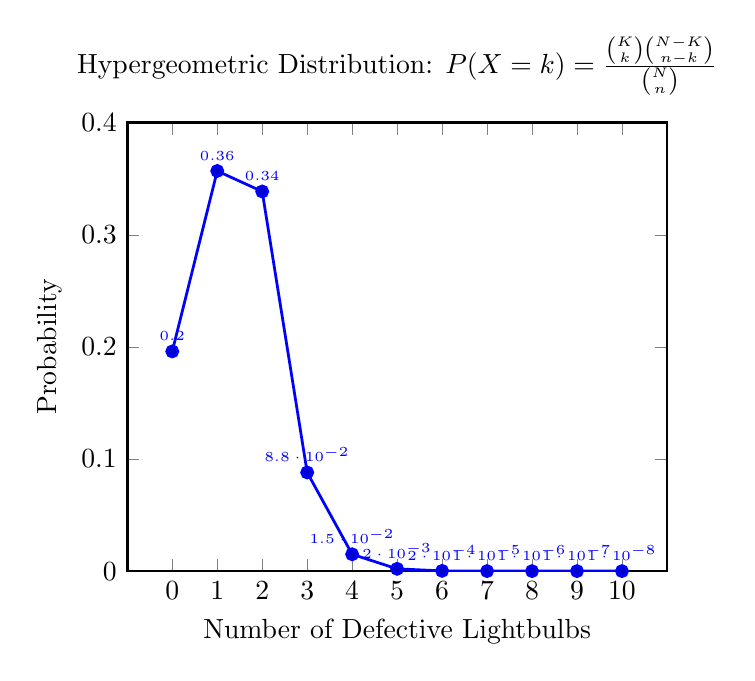
\begin{tikzpicture}
        \begin{axis}[
            line width=1pt,
            title={Hypergeometric Distribution: $P(X = k) = \frac{\binom{K}{k} \binom{N-K}{n-k}}{\binom{N}{n}}$},
            symbolic x coords={0,1,2,3,4,5,6,7,8,9,10},
            xtick=data,
            ylabel={Probability},
            xlabel={Number of Defective Lightbulbs},
            ymin=0,
            ymax=0.4,
            bar width=15pt,
            nodes near coords,
            every node near coord/.append style={font=\tiny},
        ]
        \addplot coordinates {
            (0,0.196)
            (1,0.357)
            (2,0.3387)
            (3,0.088)
            (4,0.015)
            (5,0.002)
            (6,0.0002)
            (7,0.00001)
            (8,0.000001)
            (9,0.0000001)
            (10,0.00000001)
        };
        \end{axis}
        \end{tikzpicture}
    \end{figure}
    \end{mynote}
    \item A fair die is thrown 10 times. We need to find the probability that each of 1,2,3,4 appear twice while 5 and 6 appear once each. 
    Let the events be defined as follows:
    $A_i$: Face $i$ appears on the die. \\
    We have -
    \begin{itemize}
        \item Total number of outcomes when a fair die is thrown 10 times = $6^{10}$
        \item Number of favorable outcomes where each of 1,2,3,4 appear twice while 5 and 6 appear once each = $\frac{10!}{2!2!2!2!1!1!}$
        \item Thus, the probability that each of 1,2,3,4 appear twice while 5 and 6 appear once each is given by -
        \[P = \frac{\frac{10!}{2!2!2!2!1!1!}}{6^{10}}\]
        \[\boxed{= \frac{113400}{60466176} \approx 0.001874
        }\]
    \end{itemize}
\end{enumerate}
\chapter{}
\begin{enumerate}
    \item We have the frequency table as follows - 
    \begin{center}
        \begin{tabular}{|c|ccccc|}
            \hline
            Expenditure in Rs. & 40-59 & 60 -79 & 80-99 & 100-119 & 120-139 \\
            \hline
            No. of families & 50 & $x_1$ & 500 & $x_2$ & 50 \\
            \hline
        \end{tabular}
    \end{center}
    \begin{enumerate}
        \item We have thhe mean given as Rs. 87.5. We need to find the values of $x_1$ and $x_2$. We have -
    \[\mu = \frac{\sum f_i x_i}{\sum f_i}\]
    where $f_i$ is the frequency and $x_i$ is the mid-point of the class interval. Thus, we have -
    \[87.5 = \frac{50 \cdot 49.5 + x_1 \cdot 69.5 + 500 \cdot 89.5 + x_2 \cdot 109.5 + 50 \cdot 129.5}{50 + x_1 + 500 + x_2 + 50}\]
    \[87.5 (600 + x_1 + x_2) = 2475 + 69.5 x_1 + 44750 + 109.5 x_2 + 6475\]
    \[52500 + 87.5 x_1 + 87.5 x_2 = 53700 + 69.5 x_1 + 109.5 x_2\]
    \[18 x_1 - 22 x_2 = 1200\]
    \[9 x_1 - 11 x_2 = 600 \quad \ldots (1)\]
    We also have the total number of families as 1000. Thus, we have -
    \[50 + x_1 + 500 + x_2 + 50 = 1000\]
    \[x_1 + x_2 = 400 \quad \ldots (2)\]
    Solving equations (1) and (2), we get -
    \[x_1 = 220, \quad x_2 = 180\]
    \[\boxed{(x_1, x_2) = (220, 180)
    }\]
    \item We have the median given as Rs. 87.5. We need to find the values of $x_1$ and $x_2$. We have the cumulative frequency table as follows -
    \begin{center}
        \begin{tabular}{|c|ccccc|}
            \hline
            Expenditure in Rs. & 40-59 & 60 -79 & 80-99 & 100-119 & 120-139 \\
            \hline
            No. of families & 50 & $x_1$ & 500 & $x_2$ & 50 \\
            Cumulative frequency & 50 & $50 + x_1$ & $550 + x_1$ & $550 + x_1 + x_2$ & 1000 \\
            \hline
        \end{tabular}
    \end{center}
    We know that the median class is the class where the cumulative frequency is greater than or equal to $\frac{N}{2}$. Here, $N = 1000$. Thus, we have -
    \[\frac{N}{2} = 500\]   
    Thus, the median class is 80-99. We have -
    \[\text{Median} = L + \left(\frac{\frac{N}{2} - F}{f_m}\right) \cdot h\]
    where $L$ is the lower limit of the median class, $N$ is the total number of observations, $F$ is the cumulative frequency of the class preceding the median class, $f_m$ is the frequency of the median class and $h$ is the class width. Thus, we have -
    \[87.5 = 79.5 + \left(\frac{500 - (50 + x_1)}{500}\right) \cdot 20\]
    \[8 = \left(\frac{450 - x_1}{500}\right) \cdot 20\]
    \[2000 = 9000 - 20 x_1\]
    \[20 x_1 = 7000\]
    \[x_1 = 350 \quad \ldots (1)\]
    We also have the total number of families as 1000. Thus, we have -
    \[50 + x_1 + 500 + x_2 + 50 = 1000\]
    \[x_1 + x_2 = 400 \quad \ldots (2)\]
    Solving equations (1) and (2), we get -
    \[x_1 = 350, \quad x_2 = 50\]
    \[\boxed{(x_1, x_2) = (350, 50)
    }\]
    \item We have the mode given as Rs. 87.5. We need to find the values of $x_1$ and $x_2$. We have the cumulative frequency table as follows -
    \begin{center}
        \begin{tabular}{|c|ccccc|}
            \hline
            Expenditure in Rs. & 40-59 & 60 -79 & 80-99 & 100-119 & 120-139 \\
            \hline
            No. of families & 50 & $x_1$ & 500 & $x_2$ & 50 \\
            Cumulative frequency & 50 & $50 + x_1$ & $550 + x_1$ & $550 + x_1 + x_2$ & 1000 \\
            \hline
        \end{tabular}
    \end{center}
    We know that the modal class is the class with the highest frequency. Here, the modal class is 80-99. We have -
    \[\text{Mode} = L + \left(\frac{f_1 - f_0}{2f_1 - f_0 - f_2}\right) \cdot h\]
    where $L$ is the lower limit of the modal class, $f_1$ is the frequency of the modal class, $f_0$ is the frequency of the class preceding the modal class, $f_2$ is the frequency of the class succeeding the modal class and $h$ is the class width. Thus, we have -
    \[87.5 = 79.5 + \left(\frac{500 - x_1}{2 \cdot 500 - x_1 - x_2}\right) \cdot 20\]
    \[8 = \left(\frac{500 - x_1}{1000 - x_1 - x_2}\right) \cdot 20\]
    \[4000 = 10000 - 20 x_1 - 20 x_2\]
    \[20 x_1 + 20 x_2 = 6000\]
    \[x_1 + x_2 = 300 \quad \ldots (1)\]
    We also have the total number of families as 1000. Thus, we have -
    \[50 + x_1 + 500 + x_2 + 50 = 1000\]
    \[x_1 + x_2 = 400 \quad \ldots (2)\]
    Solving equations (1) and (2), we get a contradiction. Thus, there is no solution for $x_1$ and $x_2$ such that the mode is Rs. 87.5.
    \[\boxed{\text{No solution for } (x_1, x_2)
    }\]
    \end{enumerate}
    \item We have that the values of a variable are in G.P, i.e., $a, ar, ar^2, ar^3, \ldots, ar^{n-1}$. We need to show that A.M., G.M. and H.M. are in G.P. We have -
    \begin{enumerate}
        \item Arithmetic Mean (A.M.) is given by -
        \[A.M. = \frac{a + ar + ar^2 + ar^3 + \ldots + ar^{n-1}}{n} = \frac{a(1 + r + r^2 + r^3 + \ldots + r^{n-1})}{n}\]
        \[= \frac{a\left(\frac{r^n - 1}{r - 1}\right)}{n} = \frac{a(r^n - 1)}{n(r - 1)}\]
        \item Geometric Mean (G.M.) is given by -
        \[G.M. = (a \cdot ar \cdot ar^2 \cdot ar^3 \cdot \ldots \cdot ar^{n-1})^{\frac{1}{n}} = (a^n r^{\frac{n(n-1)}{2}})^{\frac{1}{n}} = a r^{\frac{n-1}{2}}\]
        \item Harmonic Mean (H.M.) is given by -
        \[H.M. = \frac{n}{\frac{1}{a} + \frac{1}{ar} + \frac{1}{ar^2} + \frac{1}{ar^3} + \ldots + \frac{1}{ar^{n-1}}} = \frac{n}{\frac{1}{a}(1 + \frac{1}{r} + \frac{1}{r^2} + \ldots + \frac{1}{r^{n-1}})}\]
        \[= \frac{na}{\left(\frac{1 - \frac{1}{r^n}}{1 - \frac{1}{r}}\right)} = \frac{na(r - 1)r^{n-1}}{r^n - 1}\]
    \end{enumerate}
    We need to show that A.M., G.M. and H.M. are in G.P. Thus, we need to show that -
    \[(G.M.)^2 = A.M. \cdot H.M.\]
    We have -
    \[(G.M.)^2 = (a r^{\frac{n-1}{2}})^2 = a^2 r^{n-1}\]
    \[A.M. \cdot H.M. = \left(\frac{a(r^n - 1)}{n(r - 1)}\right) \cdot \left(\frac{na(r - 1)r^{n-1}}{r^n - 1}\right) = a^2 r^{n-1}\]
    Thus, we have shown that -
    \[(G.M.)^2 = A.M. \cdot H.M.\]
    Therefore, A.M., G.M. and H.M. are in G.P.
    \item We have the frequency of a variable assuming value $i$ for $i = 1, 2, \ldots, 7$ is given by $f(i) = i^2$. We need to find the mean of the variable, that is $E(X)$. We have -
    \[E(X) = \frac{\sum_{i=1}^{7} i \cdot f(i)}{\sum_{i=1}^{7} f(i)} = \frac{\sum_{i=1}^{7} i \cdot i^2}{\sum_{i=1}^{7} i^2} = \frac{\sum_{i=1}^{7} i^3}{\sum_{i=1}^{7} i^2}\]
    We know that -
    \[\sum_{i=1}^{n} i^2 = \frac{n(n+1)(2n+1)}{6}\]
    \[\sum_{i=1}^{n} i^3 = \left(\frac{n(n+1)}{2}\right)^2\]
    Thus, we have -
    \[E(X) = \frac{\left(\frac{7 \cdot 8}{2}\right)^2}{\frac{7 \cdot 8 \cdot 15}{6}} = \frac{(28)^2}{140} = \frac{784}{140} = \frac{56}{10} = 5.6\]
    \[\boxed{E(X) = 5.6
    }\]
    \item We have the A.M. of $x_1, x_2, \ldots, x_5$, with $x_i \geq x_j \iff i \geq j$ as 10. We have $y_1 = 14$, $y_2 = x_1$, $y_3 = y_4 = x_2$, $y_5 = y_6 = x_3$, $y_7 = y_8 = x_4, y_9 = y_10 = x_5$. We need to show that the A.M. of $y_1, y_2, \ldots, y_{10}$ cannot be less than 10.4. 
    We have -
    \[A.M. = \frac{x_1 + x_2 + x_3 + x_4 + x_5}{5} = 10\]
    \[x_1 + x_2 + x_3 + x_4 + x_5 = 50\]
    We need to find the A.M. of $y_1, y_2, \ldots, y_{10}$. Thus, we have -
    \[A.M. = \frac{y_1 + y_2 + y_3 + y_4 + y_5 + y_6 + y_7 + y_8 + y_9 + y_{10}}{10}\]
    \[= \frac{14 + x_1 + x_2 + x_2 + x_3 + x_3 + x_4 + x_4 + x_5 + x_5}{10}\]
    \[= \frac{14 + x_1 + 2x_2 + 2x_3 + 2x_4 + 2x_5}{10}\]
    \[= \frac{14 + (x_1 + x_2 + x_3 + x_4 + x_5) + (x_2 + x_3 + x_4 + x_5)}{10}\]
    \[= \frac{14 + 50 + (x_2 + x_3 + x_4 + x_5)}{10}\]
    \[= \frac{64 + (x_2 + x_3 + x_4 + x_5)}{10}\]
    Since $x_1 \leq x_2 \leq x_3 \leq x_4 \leq x_5$, we have -
    \[x_2 + x_3 + x_4 + x_5 \geq 4x_1\]
    Thus, we have -
    \[A.M. \geq \frac{64 + 4x_1}{10}\]
    Since $x_1 + x_2 + x_3 + x_4 + x_5 = 50$, we have -
    \[x_1 \leq 10\]
    Thus, we have -
    \[A.M. \geq \frac{64 + 4 \cdot 10}{10} = \frac{64 + 40}{10} = \frac{104}{10} = 10.4\]
    \[\boxed{A.M. \geq 10.4
    }\]
    \item The mean of 50 observations is 18. Values 22 and 16 were wrongly copied as 19 and 24 respectively. We need to find the correct mean. We have -
    \[ \text{Correct Sum} = \text{Original Sum} - \text{Wrong Values} + \text{Correct Values}\]
    \[= 50 \cdot 18 - (19 + 24) + (22 + 16)\]
    \[= 900 - 43 + 38 = 895\]
    \[ \text{Correct Mean} = \frac{\text{Correct Sum}}{50} = \frac{895}{50} = 17.9\]
    \[\boxed{\text{Correct Mean} = 17.9}\]
    \item If the average monthly income of factory workers is Rs. 5200 and average income of male workers is Rs. 5400 and Rs. 4600 respectively. We need to find the percentage of male and female workers in the factory. Let the number of male workers be $m$ and the number of female workers be $f$. We have -
    \[5200(m + f) = 5400m + 4600f\]
    \[5200m + 5200f = 5400m + 4600f\]
    \[5200f - 4600f = 5400m - 5200m\]
    \[600f = 200m\]
    \[\frac{m}{f} = \frac{600}{200} = 3\]
    Thus, we have -
    \begin{enumerate}
        \item Percentage of male workers -
        \[\frac{m}{m + f} \cdot 100 = \frac{3f}{3f + f} \cdot 100 = \frac{3}{4} \cdot 100 = 75\%\]
        \[\boxed{75\%}\]
        \item Percentage of female workers -
        \[\frac{f}{m + f} \cdot 100 = \frac{f}{3f + f} \cdot 100 = \frac{1}{4} \cdot 100 = 25\%\]
        \[\boxed{25\%}\]
    \end{enumerate}
    \item A variable x takes the values 1, 2, 3, ..., k with cumulative frequencies $F_1, F_2, F_3, \ldots, F_k$ respectively. We need to show that the mean of the variable is given by -
    \[\text{Mean} = \frac{1}{N} \sum F_i\]
    where $N$ is the total number of observations. 
    \begin{proof}    
    We know that the mean of the variable is given by -
    \[\text{Mean} = \frac{1}{N} \sum_{i=1}^{k} x_i f_i\]
    where $f_i$ is the frequency of the variable taking value $x_i$. We have -
    \[f_1 = F_1\]
    \[f_2 = F_2 - F_1\]
    \[f_3 = F_3 - F_2\]
    \[\vdots\]
    \[f_k = F_k - F_{k-1}\]
    Thus, we have -
    \[\text{Mean} = \frac{1}{N} \left(1 \cdot F_1 + 2 \cdot (F_2 - F_1) + 3 \cdot (F_3 - F_2) + \ldots + k \cdot (F_k - F_{k-1})\right)\]
    \[= \frac{1}{N} \left(F_1 + 2F_2 - 2F_1 + 3F_3 - 3F_2 + \ldots + kF_k - kF_{k-1}\right)\]
    \[= \frac{1}{N} \left(kF_k + (2 - 1)F_2 + (3 - 2)F_3 + \ldots + (k - (k-1))F_{k-1} - F_1\right)\]
    \[= \frac{1}{N} \left(kF_k + F_2 + F_3 + \ldots + F_{k-1} - F_1\right)\]
    \[= \frac{1}{N} \left(F_1 + F_2 + F_3 + \ldots + F_k\right)\]
    \[\boxed{= \frac{1}{N} \sum F_i
    }\]
    \end{proof}
    \item We have a frequency table with intervals of 10 marks each. The median of the distribution is 35.5. On verification, two observations belonging to the interval 31-40 were included in the class 21-30. After correction, the median was found to be 36.5. We need to calculate the corrected frequency of the class 31-40. 
    Let the frequency of the class 21-30 be $f_1$ and the frequency of the class 31-40 be $f_2$. We have the median formula as -
    \[\text{Median} = L + \left(\frac{\frac{N}{2} - F}{f}\right) \cdot h\]
    where $L$ is the lower class boundary of the median class, $N$ is the total number of observations, $F$ is the cumulative frequency of the class preceding the median class, $f$ is the frequency of the median class and $h$ is the class width. \\
    For the initial median of 35.5, we have -
    \[35.5 = 31 + \left(\frac{\frac{N}{2} - (F + f_1)}{f_2}\right) \cdot 10\]
    \[\Rightarrow 4.5 = \left(\frac{\frac{N}{2} - F - f_1}{f_2}\right) \cdot 10\]
    \[\Rightarrow \frac{N}{2} - F - f_1 = \frac{4.5 f_2}{10} = 0.45 f_2 \quad \text{(1)}\]
    For the corrected median of 36.5, we have -
    \[36.5 = 31 + \left(\frac{\frac{N}{2} - (F + f_1 - 2)}{f_2 + 2}\right) \cdot 10\]
    \[\Rightarrow 5.5 = \left(\frac{\frac{N}{2} - F - f_1 + 2}{f_2 + 2}\right) \cdot 10\]
    \[\Rightarrow \frac{N}{2} - F - f_1 + 2 = \frac{5.5 (f_2 + 2)}{10} = 0.55 f_2 + 1.1 \quad \text{(2)}\]
    Subtracting (1) from (2), we get -
    \[2 = (0.55 f_2 + 1.1) - (0.45 f_2)\]
    \[2 = 0.1 f_2 + 1.1\]   
    \[\Rightarrow 0.9 = 0.1 f_2\]
    \[\Rightarrow f_2 = 9\]
    Therefore, the corrected frequency of the class 31-40 is given by -
    \[\boxed{f_2 + 2 = 9 + 2 = 11
    }\]
    \item The upper boundary of each class interval has a constant ratio to the lower boundary. Show that the G.M. may be expressed as 
    $$\ln G = A + \frac{k}{n} \sum_{i=1}^{r} (i-1)f_i$$
    \begin{proof}
    Let the lower boundary of the first class interval be $a$ and the common ratio be $r$. Thus, we have the class intervals as -
    \begin{itemize}
        \item Class 1: $a$ to $ar$
        \item Class 2: $ar$ to $ar^2$
        \item Class 3: $ar^2$ to $ar^3$
        \item $\ldots$
        \item Class $i$: $ar^{i-1}$ to $ar^i$
    \end{itemize}
    Let the frequency of class $i$ be $f_i$. We have the G.M. as -  
    \[\ln G = \frac{1}{N} \sum_{i=1}^{r} f_i \ln x_i\]
    where $x_i$ is the mid-point of class $i$. We have -
    \[x_i = \frac{ar^{i-1} + ar^i}{2} = \frac{a r^{i-1} (1 + r)}{2}\]
    Thus, we have -
    \[\ln G = \frac{1}{N} \sum_{i=1}^{r} f_i \ln \left(\frac{a r^{i-1} (1 + r)}{2}\right)\]
    \[= \frac{1}{N} \sum_{i=1}^{r} f_i \left(\ln a + (i-1) \ln r + \ln \frac{1 + r}{2}\right)\]
    \[= \frac{1}{N} \left(\sum_{i=1}^{r} f_i \ln a + \sum_{i=1}^{r} f_i (i-1) \ln r + \sum_{i=1}^{r} f_i \ln \frac{1 + r}{2}\right)\]
    \[= \frac{1}{N} \left(N \ln a + \ln r \sum_{i=1}^{r} f_i (i-1) + N \ln \frac{1 + r}{2}\right)\]
    \[= \ln a + \ln \frac{1 + r}{2} + \frac{\ln r}{N} \sum_{i=1}^{r} f_i (i-1)\]
    Let us denote $\ln a + \ln \frac{1 + r}{2}$ by $A$ and $\ln r$ by $k$. Thus, we have -
    \[\ln G = A + \frac{k}{N} \sum_{i=1}^{r} (i-1) f_i\]
    \[\boxed{= A + \frac{k}{n} \sum_{i=1}^{r} (i-1)f_i
    }\]
    \end{proof}
    \item In a batch of 15, 5 students failed the test. The marks of students who passed were 90, 60, 70, 80, 80, 90, 60, 50, 40, 70. We need to find median marks of all the 15 students.
    We have the marks of the 10 students who passed the test as follows -
    \begin{center}
        \begin{tabular}{|c|c|}
            \hline
            Marks & Frequency \\
            \hline
            40 & 1 \\
            50 & 1 \\
            60 & 2 \\
            70 & 2 \\
            80 & 2 \\
            90 & 2 \\
            \hline
        \end{tabular}
    \end{center}
    We need to find the median of all 15 students. Thus, we have -
    \[ \text{Median} = L + \left(\frac{\frac{N}{2} - F}{f}\right) \cdot h\]
    where $L$ is the lower class boundary of the median class, $N$ is the total number of observations, $F$ is the cumulative frequency of the class preceding the median class, $f$ is the frequency of the median class and $h$ is the class width. \\
    Here, we have -
    \[N = 15\]
    \[\frac{N}{2} = \frac{15}{2} = 7.5\]
    The median class is 60-70. Thus, we have -
    \[L = 60\]
    \[F = 2\]
    \[f = 4\]
    \[h = 10\]
    Thus, we have -
    \[ \text{Median} = 60 + \left(\frac{7.5 - 2}{4}\right) \cdot 10\]
    \[= 60 + \left(\frac{5.5}{4}\right) \cdot 10 = 60 + 13.75 = 73.75\]
    \[\boxed{\text{Median} = 73.75
    }\]
\end{enumerate}
\chapter{}
\begin{enumerate}
    \item A variable only takes values $x_1, x_2$ with equal frequencies. We need to find the mean deviation and standard deviation in terms of $x_1$ and $x_2$.
    \begin{enumerate}
        \item Mean Deviation:
        We have the mean of the variable as -
        \[\mu = \frac{x_1 + x_2}{2}\]
        Thus, we have the mean deviation as -
        \[MD = \frac{|x_1 - \mu| + |x_2 - \mu|}{2} = \frac{\left|x_1 - \frac{x_1 + x_2}{2}\right| + \left|x_2 - \frac{x_1 + x_2}{2}\right|}{2}\]
        \[= \frac{\left|\frac{x_1 - x_2}{2}\right| + \left|\frac{x_2 - x_1}{2}\right|}{2} = \frac{\frac{|x_1 - x_2|}{2} + \frac{|x_1 - x_2|}{2}}{2} = \frac{|x_1 - x_2|}{2}\]
        \[\boxed{MD = \frac{|x_1 - x_2|}{2}
        }\]
        \item Standard Deviation:
        We have the standard deviation of the variable as -
        \[\sigma = \sqrt{\frac{(x_1 - \mu)^2 + (x_2 - \mu)^2}{2}} = \sqrt{\frac{\left(x_1 - \frac{x_1 + x_2}{2}\right)^2 + \left(x_2 - \frac{x_1 + x_2}{2}\right)^2}{2}}\]
        \[= \sqrt{\frac{\left(\frac{x_1 - x_2}{2}\right)^2 + \left(\frac{x_2 - x_1}{2}\right)^2}{2}} = \sqrt{\frac{2\left(\frac{(x_1 - x_2)^2}{4}\right)}{2}} = \sqrt{\frac{(x_1 - x_2)^2}{4}} = \frac{|x_1 - x_2|}{2}\]
        \[\boxed{\sigma = \frac{|x_1 - x_2|}{2}
        }\]
    \end{enumerate}
    \item We have $3x + 4y = 5$ and the mean deviation of $x$ about its mean is 8. We need to find the mean deviation of $y$ about its mean.
    We have the equation $3x + 4y = 5$. Thus, we have -
    \[y = \frac{5 - 3x}{4}\]
    Let the mean of $x$ be $\mu_x$ and the mean of $y$ be $\mu_y$. Thus, we have -
    \[\mu_y = \frac{5 - 3\mu_x}{4}\]
    We need to find the mean deviation of $y$ about its mean, i.e., $MD_y$. We have -
    \[MD_y = E(|y - \mu_y|) = E\left(\left|\frac{5 - 3x}{4} - \frac{5 - 3\mu_x}{4}\right|\right) = E\left(\left|\frac{-3(x - \mu_x)}{4}\right|\right)\]
    \[= \frac{3}{4} E(|x - \mu_x|) = \frac{3}{4} MD_x\]
    Given that $MD_x = 8$, we have -
    \[MD_y = \frac{3}{4} \cdot 8 = 6\]
    \[\boxed{MD_y = 6
    }\]
    \item We have the number of observations as 100, with mean and sd aas 40.1 and 5 respectively. It was later found that 50 was copied instead of the correct value 40. We need to find the correct mean and sd.
    \begin{enumerate}
        \item Correct Mean:
        We have -
        \[ \text{Correct Sum} = \text{Original Sum} - \text{Wrong Value} + \text{Correct Value}\]
        \[= 100 \cdot 40.1 - 50 + 40\]
        \[= 4010 - 50 + 40 = 4000\]
        \[ \text{Correct Mean} = \frac{\text{Correct Sum}}{100} = \frac{4000}{100} = 40\]
        \[\boxed{\text{Correct Mean} = 40
        }\]
        \item Correct Standard Deviation:
        We have the formula for standard deviation as -
        \[\sigma = \sqrt{\frac{\sum x_i^2}{N} - \mu^2}\]
        where $x_i$ are the observations, $N$ is the number of observations and $\mu$ is the mean. Thus, we have -
        \[5 = \sqrt{\frac{\sum x_i^2}{100} - (40.1)^2}\]
        \[25 = \frac{\sum x_i^2}{100} - 1608.01\]
        \[\sum x_i^2 = 162833.01\]
        Now, we need to find the correct value of $\sum x_i^2$. We have -
        \[\text{Correct } \sum x_i^2 = \text{Original } \sum x_i^2 - (\text{Wrong Value})^2 + (\text{Correct Value})^2\]
        \[= 162833.01 - 50^2 + 40^2\]
        \[= 162833.01 - 2500 + 1600 = 161933.01\]
        Thus, we have the correct standard deviation as -
        \[\sigma = \sqrt{\frac{161933.01}{100} - (40)^2} = \sqrt{1619.3301 - 1600} = \sqrt{19.3301} \approx 4.396\]
        \[\boxed{\text{Correct Standard Deviation} \approx 4.396
        }\]
    \end{enumerate}
    \item We have the class intervals as 10 marks each, total number of students as 40. We have the variance and mean as 90 and 40 respectively. Two observations belonging to the interval 21-30 were included in the class 31-40. We need to find the correct variance and mean. 
    Let the frequency of the class 21-30 be $f_1$ and the frequency of the class 31-40 be $f_2$. We have the mean formula as -
    \[\mu = \frac{\sum f_i x_i}{N}\]
    where $f_i$ is the frequency of class $i$, $x_i$ is the mid-point of class $i$ and $N$ is the total number of observations. \\
    For the initial mean of 40, we have -
    \[40 = \frac{\sum f_i x_i}{40}\]
    \[\Rightarrow \sum f_i x_i = 1600 \quad \text{(1)}\]
    For the corrected mean, we have -
    \[\mu = \frac{\sum f_i x_i - 2 \cdot 25 + 2 \cdot 35}{40} = \frac{\sum f_i x_i + 20}{40}\]
    \[\Rightarrow \mu = \frac{1600 + 20}{40} = \frac{1620}{40} = 40.5\]
    \[\boxed{\text{Correct Mean} = 40.5
    }\]
    We have the variance formula as -
    \[\sigma^2 = \frac{\sum f_i x_i^2}{N} - \mu^2\]
    where $f_i$ is the frequency of class $i$, $x_i$ is the mid-point of class $i$ and $N$ is the total number of observations. \\
    For the initial variance of 90, we have -
    \[90 = \frac{\sum f_i x_i^2}{40} - (40)^2\] 
    \[\Rightarrow \sum f_i x_i^2 = (90 + 1600) \cdot 40 =  67600 \quad \text{(2)}\]
    For the corrected variance, we have -
    \[\sigma^2 = \frac{\sum f_i x_i^2 - 2 \cdot 25^2 + 2 \cdot 35^2}{40} - (40.5)^2\]
    \[\Rightarrow \sigma^2 = \frac{67600 - 1250 + 2450}{40} - 1640.25\]
    \[\Rightarrow \sigma^2 = \frac{68800}{40} - 1640.25 = 1720 - 1640.25 = 79.75\]
    \[\boxed{\text{Correct Variance} = 79.75
    }\]
    \item The mean square deviation around 1 and -1 is 3 and 7 respectively. We need to find the sd of the observations. 
    Let the mean of the observations be $\mu$. We have the mean square deviation around 1 as -
    \[MSD_1 = \frac{\sum (x_i - 1)^2}{N} = 3\]
    \[\Rightarrow \sum (x_i - 1)^2 = 3N\]
    \[\Rightarrow \sum (x_i^2 - 2x_i + 1) = 3N\]
    \[\Rightarrow \sum x_i^2 - 2 \sum x_i + N = 3N\]
    \[\Rightarrow \sum x_i^2 - 2N\mu + N = 3N\]
    \[\Rightarrow \sum x_i^2 = 2N\mu + 2N \quad \text{(1)}\]
    We have the mean square deviation around -1 as -
    \[MSD_{-1} = \frac{\sum (x_i + 1)^2}{N} = 7\]
    \[\Rightarrow \sum (x_i + 1)^2 = 7N\]
    \[\Rightarrow \sum (x_i^2 + 2x_i + 1) = 7N\]
    \[\Rightarrow \sum x_i^2 + 2 \sum x_i + N = 7N\]
    \[\Rightarrow \sum x_i^2 + 2N\mu + N = 7N\]
    \[\Rightarrow \sum x_i^2 = -2N\mu + 6N \quad \text{(2)}\]
    Solving equations (1) and (2), we get -
    \[2N\mu + 2N = -2N\mu + 6N\]
    \[\Rightarrow 4N\mu = 4N\]
    \[\Rightarrow \mu = 1\]
    Substituting the value of $\mu$ in equation (1), we get -
    \[\sum x_i^2 = 2N \cdot 1 + 2N = 4N\]
    We have the formula for standard deviation as -
    \[\sigma = \sqrt{\frac{\sum x_i^2}{N} - \mu^2}\]
    \[= \sqrt{\frac{4N}{N} - (1)^2} = \sqrt{4 - 1} = \sqrt{3}\]
    \[\boxed{\sigma = \sqrt{3}
    }\]
    \item We have the distribution as follows - 
    \begin{center}
        \begin{tabular}{|c|ccccccccc|}
            \hline
            $x$ & 0 & 1 & 2 & 3 & 4 & 5 & 6 & 7 & 8 \\
            \hline
            $f$ & 4 & 10 & 13 & 21 & 23 & 20 & 18 & 9 & 2 \\
            \hline
        \end{tabular}
    \end{center}
    We need to find the mean deviation around median for this distribution.
    We have the total number of observations as -
    \[N = 4 + 10 + 13 + 21 + 23 + 20 + 18 + 9 + 2 = 120\]
    We need to find the median of the distribution. Thus, we have -
    \[\frac{N}{2} = \frac{120}{2} = 60\]
    The median class is 4. Thus, we have -
    \[L = 4\]
    \[F = 4 + 10 + 13 + 21 = 48\]
    \[f = 23\]
    \[h = 1\]
    Thus, we have -
    \[ \text{Median} = 4 + \left(\frac{60 - 48}{23}\right) \cdot 1 = 4 + \frac{12}{23} = \frac{92 + 12}{23} = \frac{104}{23} \approx 4.52\]
    Now, we need to find the mean deviation around median. Thus, we have -
    \[MD = \frac{\sum f_i |x_i - \text{Median}|}{N}\]
    \begin{multline}
= \frac{4 \left|0 - \frac{104}{23}\right| + 10 \left|1 - \frac{104}{23}\right| + 13 \left|2 - \frac{104}{23}\right| + 21 \left|3 - \frac{104}{23}\right| + 23 \left|4 - \frac{104}{23}\right| + 20 \left|5 - \frac{104}{23}\right|}{120} \\ + \frac{18 \left|6 - \frac{104}{23}\right| + 9 \left|7 - \frac{104}{23}\right| + 2 \left|8 - \frac{104}{23}\right|}{120}
        \end{multline}
        \begin{multline}
= \frac{4 \cdot \frac{104}{23} + 10 \cdot \frac{81}{23} + 13 \cdot \frac{58}{23} + 21 \cdot \frac{35}{23} + 23 \cdot \frac{12}{23} + 20 \cdot \frac{19}{23} + 18 \cdot \frac{42}{23} + 9 \cdot \frac{65}{23} + 2 \cdot \frac{88}{23}}{120} \\
= \frac{\frac{416 + 810 + 754 + 735 + 276 + 380 + 756 + 585 + 176}{23}}{120} = \frac{\frac{4888}{23}}{120} = \frac{4888}{2760} = \frac{1222}{690} \approx 1.77
        \end{multline}
    \item In a batch of 10 children, IQ of a dull boy is 36 below the average IQ of the batch. Show that the sd of IQ for all children cannot be less that 10.8. If the sd is 11.4, we need to find the sd without the dull boy. 
    We have the mean IQ of the batch as $\mu$. Thus, we have the IQ of the dull boy as $\mu - 36$. We need to show that the sd of IQ for all children cannot be less than 10.8.
    We have the formula for standard deviation as -
    \[\sigma = \sqrt{\frac{\sum (x_i - \mu)^2}{N}}\]
    where $x_i$ are the observations, $N$ is the number of observations and $\mu$ is the mean. \\
    Thus, we have -
    \[\sigma^2 = \frac{\sum (x_i - \mu)^2
}{N}\]
    \[\Rightarrow \sum (x_i - \mu)^2 = N \sigma^2\]
    \[\Rightarrow \sum (x_i - \mu)^2 = 10 \sigma^2 \quad \text{(1)}\]
    We know that -
    \[(x_i - \mu)^2 \geq 0\]
    Thus, we have -
    \[(\mu - 36 - \mu)^2 \leq \sum (x_i - \mu)^2\]
    \[\Rightarrow 1296 \leq 10 \sigma^2\]
    \[\Rightarrow \sigma^2 \geq 129.6\]
    \[\Rightarrow \sigma \geq \sqrt{129.6} = 10.8\]
    Thus, we have shown that the sd of IQ for all children cannot be less than 10.8. 
    Now, we need to find the sd without the dull boy.
    We have the formula for standard deviation as -
    \[\sigma = \sqrt{\frac{\sum (x_i - \mu)^2}{N}}\]
    where $x_i$ are the observations, $N$ is the number of observations and $\mu$ is the mean. \\
    We have the mean after removing the dull boy as - 
    $$\mu' = \frac{10\mu - (\mu - 36)}{9} = \frac{9\mu + 36}{9} = \mu + 4$$
    We have the sum of squares after removing the dull boy as -
    \[\sum (x_i - \mu')^2 = \sum (x_i - \mu + \mu - \mu')^2\]
    \[= \sum (x_i - \mu - 4)^2 = \sum (x_i - \mu)^2 - 8 \sum (x_i - \mu) + 16N\]
    \[= \sum (x_i - \mu)^2 + 16N\]
    \[= 10 \sigma^2 + 160 \quad \text{(2)}\]
    Thus, we have the sd without the dull boy as -
    \[\sigma' = \sqrt{\frac{\sum (x_i - \mu')^2}{N - 1}} = \sqrt{\frac{10 \sigma^2 + 160}{9}}\]
    Given that $\sigma = 11.4$, we have -
    \[\sigma' = \sqrt{\frac{10 \cdot (11.4)^2 + 160}{9}} = \sqrt{\frac{10 \cdot 129.96 + 160}{9}} = \sqrt{\frac{1299.6 + 160}{9}} = \sqrt{\frac{1459.6}{9}} \approx \sqrt{162.18} \approx 12.74\]
    \[\boxed{\sigma' \approx 12.74
    }\]
    \item We have the Distribution as follows -
    \begin{center}
        \begin{tabular}{|c|cccccc|}
            \hline 
            Age (in years) & 20-25 & 25-30 & 30-35 & 35-40 & 40-45 & 45-50 \\
            \hline
            No. of persons & 110 & 90 & 75 & 55 & 40 & 30 \\
            \hline
        \end{tabular}
    \end{center}
    We need to find the mean deviation about median and sd for the above distribution.
    We have the total number of persons as -
    \[N = 110 + 90 + 75 + 55 + 40 + 30 = 400\]
    We need to find the median of the distribution. Thus, we have -
    \[\frac{N}{2} = \frac{400}{2} = 200\]
    The median class is 30-35. Thus, we have -
    \[L = 30\]
    \[F = 110 + 90 = 200\]
    \[f = 75\]
    \[h = 5\]
    Thus, we have -
    \[ \text{Median} = 30 + \left(\frac{200 - 200}{75}\right) \cdot 5 = 30 + 0 = 30\]
    Now, we need to find the mean deviation about median. Thus, we have -
    \[MD = \frac{\sum f_i |x_i - \text{Median}|}{N}\]
    \[= \frac{110 |22.5 - 30| + 90 |27.5 - 30| + 75 |32.5 - 30| + 55 |37.5 - 30| + 40 |42.5 - 30| + 30 |47.5 - 30|}{400}\]
    \[= \frac{110 \cdot 7.5 + 90 \cdot 2.5 + 75 \cdot 2.5 + 55 \cdot 7.5 + 40 \cdot 12.5 + 30 \cdot 17.5}{400}\]
    \[= \frac{825 + 225 + 187.5 + 412.5 + 500 + 525}{400} = \frac{2675}{400} = 6.6875\]
    \[\boxed{MD \approx 6.69
    }\]
    Now, we need to find the sd for the distribution. We have the formula for standard deviation as -
    \[\sigma = \sqrt{\frac{\sum f_i x_i^2}{N} - \mu^2}\]
    where $f_i$ is the frequency of class $i$, $x_i$ is the mid-point of class $i$ and $N$ is the total number of observations. \\
    We have the mean as -
    \[\mu = \frac{\sum f_i x_i}{N} = \frac{110 \cdot 22.5 + 90 \cdot 27.5 + 75 \cdot 32.5 + 55 \cdot 37.5 + 40 \cdot 42.5 + 30 \cdot 47.5}{400}\]
    \[= \frac{2475 + 2475 + 2437.5 + 2062.5 + 1700 + 1425}{400} = \frac{15575}{400} = 38.9375\]
    Now, we have -
    \[\sum f_i x_i^2 = 110 \cdot (22.5)^2 + 90 \cdot (27.5)^2 + 75 \cdot (32.5)^2 + 55 \cdot (37.5)^2 + 40 \cdot (42.5)^2 + 30 \cdot (47.5)^2\]
    \[= 110 \cdot 506.25 + 90 \cdot 756.25 + 75 \cdot 1056.25 + 55 \cdot 1406.25 + 40 \cdot 1806.25 + 30 \cdot 2256.25\]
    \[= 55687.5 + 68062.5 + 79218.75 + 77343.75 + 72250 + 67687.5 = 420250\]
    Thus, we have the sd as -
    \[\sigma = \sqrt{\frac{420250}{400} - (38.9375)^2} = \sqrt{1050.625 - 1516.015625}\approx 7.29 \]
    \[\boxed{\sigma \approx 7.29
    }\]
    \item We have two groups of 15, 22 with variances 9 and 16 respectively. We have that their means differ by 8.8. We need to find the sd of the combined group.
    We have the formula for standard deviation of combined group as -
    \[\sigma_c = \sqrt{\frac{(n_1 - 1) \sigma_1^2 + (n_2 - 1) \sigma_2^2 + \frac{n_1 n_2}{n_1 + n_2} (\mu_1 - \mu_2)^2}{n_1 + n_2 - 1}}\]
    where $n_1, n_2$ are the number of observations in group 1 and group 2 respectively, $\sigma_1, \sigma_2$ are the standard deviations of group 1 and group 2 respectively and $\mu_1, \mu_2$ are the means of group 1 and group 2 respectively. \\
    Thus, we have -
    \[\sigma_c = \sqrt{\frac{(15 - 1) \cdot 9 + (22 - 1) \cdot 16 + \frac{15 \cdot 22}{15 + 22} \cdot (8.8)^2}{15 + 22 - 1}}\]
    \[= \sqrt{\frac{14 \cdot 9 + 21 \cdot 16 + \frac{330}{37} \cdot 77.44}{36}}\]
    \[= \sqrt{\frac{126 + 336 + 691.2}{36}} = \sqrt{\frac{1153.2}{36}} \approx \sqrt{32.0333} \approx 5.66\]
    \[\boxed{\sigma_c \approx 5.66
    }\]
    \item We need to show that if a single observation $x$ is added to a set of $n$ observations with mean $\bar{x}$ and variance $s^2$, then the new variance will be larger than the old if $$|x - \bar{x}| > s \sqrt{\frac{n+1}{n}}$$
    \begin{proof}
    Let the new mean after adding the observation $x$ be $\bar{x'}$ and the new variance be $s'^2$. We have -
    \[\bar{x'} = \frac{n \bar{x} + x}{n + 1}\]
    We have the formula for variance as -
    \[s^2 = \frac{\sum (x_i - \bar{x})^2}{n}\]
    where $x_i$ are the observations and $n$ is the number of observations. \\
    Thus, we have -
    \[s'^2 = \frac{\sum (x_i - \bar{x'})^2 + (x - \bar{x'})^2}{n + 1}\]
    \[= \frac{\sum (x_i - \bar{x} + \bar{x} - \bar{x'})^2 + (x - \bar{x'})^2}{n + 1}\]
    \[= \frac{\sum (x_i - \bar{x})^2 + 2(\bar{x} - \bar{x'}) \sum (x_i - \bar{x}) + n(\bar{x} - \bar{x'})^2 + (x - \bar{x'})^2}{n + 1}\]
    \[= \frac{n s^2 + n(\bar{x} - \bar{x'})^2 + (x - \bar{x'})^2}{n + 1}\]
    We need to show that $s'^2 > s^2$. Thus, we have -
    \[\frac{n s^2 + n(\bar{x} - \bar{x'})^2 + (x - \bar{x'})^2}{n + 1} > s^2\]
    \[\Rightarrow n s^2 + n(\bar{x} - \bar{x'})^2 + (x - \bar{x'})^2 > (n + 1) s^2\]
    \[\Rightarrow n(\bar{x} - \bar{x'})^2 + (x - \bar{x'})^2 > s^2\]
    Substituting the value of $\bar{x'}$, we get -
    \[n\left(\bar{x} - \frac{n \bar{x} + x}{n + 1}\right)^2 + \left(x - \frac{n \bar{x} + x}{n + 1}\right)^2 > s^2\]
    \[\Rightarrow n\left(\frac{\bar{x} - x}{n + 1}\right)^2 + \left(\frac{x - \bar{x}}{n + 1}\right)^2 > s^2\]
    \[\Rightarrow \frac{n (x - \bar{x})^2 + (x - \bar{x})^2}{(n + 1)^2} > s^2\]
    \[\Rightarrow \frac{(n + 1)(x - \bar{x})^2}{(n + 1)^2} > s^2\]
    \[\Rightarrow \frac{(x - \bar{x})^2}{n + 1} > s^2\]
    \[\Rightarrow |x - \bar{x}| > s \sqrt{n + 1}\]
    \[\Rightarrow |x - \bar{x}| > s \sqrt{\frac{n + 1}{n}}\]
    Thus, we have shown that if a single observation $x$ is added to a set of $n$ observations with mean $\bar{x}$ and variance $s^2$, then the new variance will be larger than the old if $$|x - \bar{x}| > s \sqrt{\frac{n+1}{n}}$$
    \end{proof}
\end{enumerate}
\chapter{}
\begin{enumerate}
    \item The mean, mode and coefficient of variation of the weekly wages of a group of workers are Rs. 50, Rs. 58 and 40\% respectively. We need to find the sd and median and coefficient of skewness of the weekly wages.
    \begin{enumerate}
        \item Standard Deviation:
        We have the formula for coefficient of variation as -
        \[CV = \frac{\sigma}{\mu} \cdot 100\]
        where $\sigma$ is the standard deviation and $\mu$ is the mean. \\
        Substituting the values, we get -
        \[40 = \frac{\sigma}{50} \cdot 100\]
        \[\Rightarrow \sigma = \frac{40 \cdot 50}{100} = 20\]
        Thus, the standard deviation is Rs. 20.
        \[\boxed{\sigma = 20
        }\]
        \item Median:
        We have the formula for median in terms of mean and mode as -
        \[\text{Median} = 3 \cdot \text{Mode} - 2 \cdot \text{Mean}\]
        \[= 3 \cdot 58 - 2 \cdot 50
        = 174 - 100 = 74\]
        Thus, the median is Rs. 74.
        \[\boxed{\text{Median} = 74
        }\]
        \item Coefficient of Skewness:
        We have the formula for coefficient of skewness as -
        \[Sk = \frac{3(\mu - \text{Median})}{\sigma}\]
        \[= \frac{3(50 - 74)}{20} = \frac{3(-24)}{20} = \frac{-72}{20} = -3.6\]
        Thus, the coefficient of skewness is -3.6.
        \[\boxed{Sk = -3.6
        }\]
    \end{enumerate}
    \item In a moderately skewed distribution, the mean is 50, median is 53 and coefficient of variation is 20\%. We need to find the value of coefficient of skewness.
    We have the formula for coefficient of skewness as -
    \[Sk = \frac{3(\mu - \text{Median})}{\sigma}\]
    We have the mean as $\mu = 50$ and median as 53. We need to find the standard deviation $\sigma$. We have the formula for coefficient of variation as -
    \[CV = \frac{\sigma}{\mu} \cdot 100\]
    Substituting the values, we get -
    \[20 = \frac{\sigma}{50} \cdot 100\]
    \[\Rightarrow \sigma = \frac{20 \cdot 50}{100} = 10\]
    Now, substituting the values in the formula for coefficient of skewness, we get -
    \[Sk = \frac{3(50 - 53)}{10} = \frac{3(-3)}{10} = \frac{-9}{10} = -0.9\]
    Thus, the coefficient of skewness is -0.9.
    \[\boxed{Sk = -0.9
    }\]
    \item We have sd of a distribution as 3. We need to calculate the value of $\mu_4$ such that the distribution is - 
    \begin{enumerate}
        \item Leptokurtic: 
        We have the condition for leptokurtic distribution as -
        \[\frac{\mu_4}{\sigma^4} > 3\]
        where $\mu_4$ is the fourth central moment and $\sigma$ is the standard deviation. \\
        Substituting the value of $\sigma$, we get -
        \[\frac{\mu_4}{3^4} > 3\]
        \[\Rightarrow \frac{\mu_4}{81} > 3\]
        \[\Rightarrow \mu_4 > 243\]
        Thus, for the distribution to be leptokurtic, $\mu_4$ should be greater than 243.
        \[\boxed{\mu_4 > 243
        }\]
        \item Mesokurtic:
        We have the condition for mesokurtic distribution as -
        \[\frac{\mu_4}{\sigma^4} = 3\]
        where $\mu_4$ is the fourth central moment and $\sigma$ is the standard deviation. \\
        Substituting the value of $\sigma$, we get -
        \[\frac{\mu_4}{3^4} = 3\]
        \[\Rightarrow \frac{\mu_4}{81} = 3\]
        \[\Rightarrow \mu_4 = 243\]
        Thus, for the distribution to be mesokurtic, $\mu_4$ should be equal to 243.
        \[\boxed{\mu_4 = 243
        }\]
        \item Platykurtic:
        Similarly, we have the condition for platykurtic distribution as -
        \[\frac{\mu_4}{\sigma^4} < 3\]
        where $\mu_4$ is the fourth central moment and $\sigma$ is the standard deviation. \\
        Same as parts (a) and (b), we get -
        \[\mu_4 < 243\]
        Thus, for the distribution to be platykurtic, $\mu_4$ should be less than 243.
        \[\boxed{\mu_4 < 243
        }\]
    \end{enumerate}
    \item We need to verify whether the data is consistent or not. We have the data as follows - 
    \begin{enumerate}
        \item $m_2 = 16, m_3 = -64, m_4 = 162$ \\
        We have the formula for central moments in terms of raw moments as -
        \[\mu_2 = m_2 - m_1^2\]
        \[\mu_3 = m_3 - 3m_1 m_2 + 2m_1^3\]
        \[\mu_4 = m_4 - 4m_1 m_3 + 6m_1^2 m_2 - 3m_1^4\]
        where $\mu_n$ is the $n^{th}$ central moment and $m_n$ is the $n^{th}$ raw moment. \\
        We need to find the value of $m_1$. We have the condition for consistency as -
        \[\mu_4 \geq \mu_2^2\]
        Substituting the values, we get -
        \[162 \geq (16 - m_1^2)^2\]
        \[\Rightarrow 162 \geq 256 - 32m_1^2 + m_1^4\]
        \[\Rightarrow m_1^4 - 32m_1^2 + 94 \leq 0\]
        \[\Rightarrow (m_1^2 - 2)(m_1^2 - 30) \leq 0\]
        \[\Rightarrow 2 \leq m_1^2 \leq 30\]
        \[\Rightarrow \sqrt{2} \leq |m_1| \leq \sqrt{30}\]
        Thus, the data is consistent for $|m_1|$ in the range \[\sqrt{2}, \sqrt{30}\].
        \item Mean = 63, Median = 65, coefficient of skewness = -0.375, Variance=576. \\
        We have the formula for coefficient of skewness as -
        \[Sk = \frac{3(\mu - \text{Median})}{\sigma}\]
        where $\mu$ is the mean and $\sigma$ is the standard deviation. \\
        We have the standard deviation as -
        \[\sigma = \sqrt{576} = 24\]
        Substituting the values, we get -
        \[-0.375 = \frac{3(63 - 65)}{24}\]
        \[-0.375 = \frac{3(-2)}{24}\]
        \[-0.375 = -0.25\]
        Thus, the data is not consistent.
        \[\boxed{\text{Data is not consistent}
        }\]
        \item $b_1 = 0.7, b_2 = 15$ \\
        We have the formula for coefficient of skewness in terms of moments as -
        \[b_1 = \frac{\mu_3^2}{\mu_2^3}\]
        \[b_2 = \frac{\mu_4}{\mu_2^2}\]
        where $\mu_n$ is the $n^{th}$ central moment. \\
        We need to find the value of $\mu_2$. We have the condition for consistency as -
        \[b_2 \geq b_1 + 1\]
        Substituting the values, we get -
        \[15 \geq 0.7 + 1\]
        \[15 \geq 1.7\]
        Thus, the data is consistent.
        \[\boxed{\text{Data is consistent}
        }\]
    \end{enumerate}
    \item The measure of skewness is 0.32. It is also known that the mean and variance are 29.6 and 42.25. We need to find the median and mode of the distribution.
    We have the formula for coefficient of skewness as -
    \[Sk = \frac{3(\mu - \text{Median})}{\sigma}\]
    where $\mu$ is the mean and $\sigma$ is the standard deviation. \\
    We have the standard deviation as -
    \[\sigma = \sqrt{42.25} = 6.5\]
    Substituting the values, we get -
    \[0.32 = \frac{3(29.6 - \text{Median})}{6.5}\]
    \[\Rightarrow 0.32 \cdot 6.5 = 3(29.6 - \text{Median})\]
    \[\Rightarrow 2.08 = 88.8 - 3 \cdot \text{Median}\]
    \[\Rightarrow 3 \cdot \text{Median} = 88.8 - 2.08 = 86.72\]
    \[\Rightarrow \text{Median} = \frac{86.72}{3} \approx 28.91\]
    \[\boxed{\text{Median} \approx 28.91
    }\]
    We have the formula for mode in terms of mean and median as -
    \[\text{Mode} = 3 \cdot \text{Median} - 2 \cdot \mu\]
    \[= 3 \cdot 28.91 - 2 \cdot 29.6\]
    \[= 86.73 - 59.2 = 27.53\]
    \[\boxed{\text{Mode} \approx 27.53
    }\]
    \item We have the mean as 120, mode as 123, and coefficient of skewness as -0.3. We need to find the coefficient of variation. 
    We have the formula for coefficient of skewness as -
    \[Sk = \frac{3(\mu - \text{Median})}{\sigma}\]
    where $\mu$ is the mean and $\sigma$ is the standard deviation. \\
    We need to find the median first. Substituting the values, we get -
    \[-0.3 = \frac{3(120 - \text{Median})}{\sigma}\]
    \[\Rightarrow -0.3 \sigma = 3(120 - \text{Median})\]
    \[\Rightarrow -0.1 \sigma = 120 - \text{Median}\]
    \[\Rightarrow \text{Median} = 120 + 0.1 \sigma \quad \text{(1)}\]
    We have the formula for mode in terms of mean and median as -
    \[\text{Mode} = 3 \cdot \text{Median} - 2 \cdot \mu\]
    Substituting the values, we get -
    \[123 = 3 \cdot \text{Median} - 2 \cdot 120\]
    \[\Rightarrow 123 = 3 \cdot \text{Median} - 240\]
    \[\Rightarrow 3 \cdot \text{Median} = 363\]
    \[\Rightarrow \text{Median} = 121 \quad \text{(2)}\]
    Solving equations (1) and (2), we get -
    \[121 = 120 + 0.1 \sigma\]
    \[\Rightarrow 0.1 \sigma = 1\]
    \[\Rightarrow \sigma = 10\]
    We have the formula for coefficient of variation as -
    \[CV = \frac{\sigma}{\mu} \times 100\]
    Substituting the values, we get -
    \[CV = \frac{10}{120} \times 100 = \frac{1000}{120} \approx 8.33\%\]
    \[\boxed{CV \approx 8.33\%}\]
    \item We have that a variable $X$ takes on only 2 values with equal frequency. We need to find $\mu_2, \mu_3$ and $\mu_4$ in terms of $a$ and $b$ where the two values are $a$ and $b$.
    Let the two values be $a$ and $b$. We have the mean as -
    \[\mu = \frac{a + b}{2}\]
    We have the formula for $n^{th}$ central moment as -
    \[\mu_n = \frac{(a - \mu)^n + (b - \mu)^n}{2}\]
    We now calculate $\mu_2, \mu_3$ and $\mu_4$ as follows -
    \begin{enumerate}
        \item $\mu_2$:
        \[\mu_2 = \frac{(a - \mu)^2 + (b - \mu)^2}{2}\]
        \[= \frac{\left(a - \frac{a + b}{2}\right)^2 + \left(b - \frac{a + b}{2}\right)^2}{2}\]
        \[= \frac{\left(\frac{a - b}{2}\right)^2 + \left(\frac{b - a}{2}\right)^2}{2} = \frac{\frac{(a - b)^2}{4} + \frac{(b - a)^2}{4}}{2} = \frac{\frac{(a - b)^2}{4} + \frac{(a - b)^2}{4}}{2} = \frac{\frac{2(a - b)^2}{4}}{2} = \frac{(a - b)^2}{4}\]
        \[\boxed{\mu_2 = \frac{(a - b)^2}{4}
        }\]
        \item $\mu_3$:
        \[\mu_3 = \frac{(a - \mu)^3 + (b - \mu)^3}{2}\]
        \[= \frac{\left(a - \frac{a + b}{2}\right)^3 + \left(b - \frac{a + b}{2}\right)^3}{2}\]
        \[= \frac{\left(\frac{a - b}{2}\right)^3 + \left(\frac{b - a}{2}\right)^3}{2} = \frac{\frac{(a - b)^3}{8} + \frac{(b - a)^3}{8}}{2} = \frac{\frac{(a - b)^3}{8} + \frac{-(a - b)^3}{8}}{2} = 0\]
        \[\boxed{\mu_3 = 0
        }\]
        \item $\mu_4$:
        \[\mu_4 = \frac{(a - \mu)^4 + (b - \mu)^4}{2}\]
        \[= \frac{\left(a - \frac{a + b}{2}\right)^4 + \left(b - \frac{a + b}{2}\right)^4}{2}\]
        \[= \frac{\left(\frac{a - b}{2}\right)^4 + \left(\frac{b - a}{2}\right)^4}{2} = \frac{\frac{(a - b)^4}{16} + \frac{(b - a)^4}{16}}{2} = \frac{\frac{(a - b)^4}{16} + \frac{(a - b)^4}{16}}{2} = \frac{\frac{2(a - b)^4}{16}}{2} = \frac{(a - b)^4}{16}\]
        \[\boxed{\mu_4 = \frac{(a - b)^4}{16}
        }\]
    \end{enumerate}
    \item We have the mean, variance and $\mu_3$ of a distribution as 10, 16, 64. We need to find the values of the first four moments around the origin, given $b_2 =4$. We have - 
    \begin{enumerate}
        \item $m_1$:
        We have the first moment around the origin as the mean. Thus, we have -
        \[\boxed{m_1 = 10
        }\]
        \item $m_2$:
        We have the formula for variance in terms of moments as -
        \[\sigma^2 = m_2 - m_1^2\]
        where $\sigma^2$ is the variance, $m_2$ is the second moment around the origin and $m_1$ is the first moment around the origin. \\
        Substituting the values, we get -
        \[16 = m_2 - 10^2\]
        \[\Rightarrow m_2 = 16 + 100 = 116\]
        \[\boxed{m_2 = 116
        }\]
        \item $m_3$:
        We have the formula for third central moment in terms of moments as -
        \[\mu_3 = m_3 - 3m_1 m_2 + 2m_1^3\]
        where $\mu_3$ is the third central moment, $m_3$ is the third moment around the origin and $m_1, m_2$ are the first and second moments around the origin respectively. \\
        Substituting the values, we get -
        \[64 = m_3 - 3 \cdot 10 \cdot 116 + 2 \cdot 10^3\]
        \[\Rightarrow 64 = m_3 - 3480 + 2000\]
        \[\Rightarrow m_3 = 64 + 3480 - 2000 = 1544\]
        \[\boxed{m_3 = 1544
        }\]
        \item $m_4$:
        We have the formula for coefficient of kurtosis in terms of moments as -
        \[b_2 = \frac{m_4 - 4m_1 m_3 + 6m_1^2 m_2 - 3m_1^4}{(m_2 - m_1^2)^2}\]
        where $b_2$ is the coefficient of kurtosis, $m_4$ is the fourth moment around the origin and $m_1, m_2, m_3$ are the first, second and third moments around the origin respectively. \\
        Substituting the values, we get -
        \[4 = \frac{m_4 - 4 \cdot 10 \cdot 1544 + 6 \cdot 10^2 \cdot 116 - 3 \cdot 10^4}{(116 - 10^2)^2}\]
        \[= \frac{m_4 - 61760 + 69600 - 30000}{16^2}\]
        \[= \frac{m_4 - 22160}{256}\]
        \[\Rightarrow 4 \cdot 256 = m_4 - 22160\]
        \[\Rightarrow m_4 = 1024 + 22160 = 23184\]
        \[\boxed{m_4 = 23184
        }\]
    \end{enumerate}
    \item We have the frequency table as follows -
    \begin{center}
        \begin{tabular}{|c|ccccccccc|}
            \hline
            Value & 0 & 1 & 2 & 3 & 4 & 5 & 6 & 7 & 8 \\
            \hline
            Frequency & 1 & 8 & 28 & 56 & 70 & 56 & 28 & 8 & 1 \\
            \hline
        \end{tabular}
    \end{center}
    We need to find the first four moments about the mean and hence find $b_1, b_2$. 
    We have the total frequency as -
    \[N = 1 + 8 + 28 + 56 + 70 + 56 + 28 + 8 + 1 = 256\]
    We have the mean as -
    \[\mu = \frac{\sum f_i x_i}{N} = \frac{1 \cdot 0 + 8 \cdot 1 + 28 \cdot 2 + 56 \cdot 3 + 70 \cdot 4 + 56 \cdot 5 + 28 \cdot 6 + 8 \cdot 7 + 1 \cdot 8}{256}\]
    \[= \frac{0 + 8 + 56 + 168 + 280 + 280 + 168 + 56 + 8}{256} = \frac{1024}{256} = 4\]
    Now, we calculate the first four moments about the mean as follows -
    \begin{enumerate}
        \item $\mu_2$:
        \[\mu_2 = \frac{\sum f_i (x_i - \mu)^2}{N}\]
        \[= \frac{1 \cdot 16 + 8 \cdot 9 + 28 \cdot 4 + 56 \cdot 1 + 70 \cdot 0 + 56 \cdot 1 + 28 \cdot 4 + 8 \cdot 9 + 1 \cdot 16}{256}\]
        \[= \frac{16 + 72 + 112 + 56 + 0 + 56 + 112 + 72 + 16}{256} = \frac{512}{256} = 2\]
        \[\boxed{\mu_2 = 2
        }\]
        \item $\mu_3$:
        \[\mu_3 = \frac{\sum f_i (x_i - \mu)^3}{N}\]
        \[= \frac{1 \cdot (-64) + 8 \cdot (-27) + 28 \cdot (-8) + 56 \cdot (-1) + 70 \cdot 0 + 56 \cdot 1 + 28 \cdot 8 + 8 \cdot 27 + 1 \cdot 64}{256}\]
        \[= \frac{-64 - 216 - 224 - 56 + 0 + 56 + 224 + 216 + 64}{256} = \frac{0}{256} = 0\]
        \[\boxed{\mu_3 = 0
        }\]
        \item $\mu_4$:
        \[\mu_4 = \frac{\sum f_i (x_i - \mu)^4}{N}\]
        \[= \frac{1 \cdot 256 + 8 \cdot 81 + 28 \cdot 16 + 56 \cdot 1 + 70 \cdot 0 + 56 \cdot 1 + 28 \cdot 16 + 8 \cdot 81 + 1 \cdot 256}{256}\]
        \[= \frac{256 + 648 + 448 + 56 + 0 + 56 + 448 + 648 + 256}{256} = \frac{2816}{256} = 11\]
        \[\boxed{\mu_4 = 11
        }\]
        \item $b_1, b_2$:
        We have the formula for coefficient of skewness as -
        \[b_1 = \frac{\mu_3^2}{\mu_2^3} = \frac{0^2}{2^3} = 0\]
        \[\boxed{b_1 = 0
        }\]
        We have the formula for coefficient of kurtosis as -
        \[b_2 = \frac{\mu_4}{\mu_2^2} = \frac{11}{2^2} = \frac{11}{4} = 2.75\]
        \[\boxed{b_2 = 2.75
        }\]
    \end{enumerate}
    \item We have the following frequency distribution -
    \begin{center}
        \begin{tabular}{|c|cccccc|}
            \hline 
            Class Interval & 21-24 & 25-28 & 29-32 & 33-36 & 37-40 & 41-44 \\
            \hline
            Frequency & 110 & 90 & 75 & 55 & 40 & 30 \\
            \hline
        \end{tabular}
    \end{center}
    We need to find the first four moments about the mean and hence find $b_1, b_2$.
    We have the total frequency as -
    \[N = 110 + 90 + 75 + 55 + 40 + 30 = 400\]
    We have the midpoints of the class intervals as follows -
    \begin{center}
        \begin{tabular}{|c|cccccc|}
            \hline 
            Class Interval & 21-24 & 25-28 & 29-32 & 33-36 & 37-40 & 41-44 \\
            \hline
            Midpoint & 22.5 & 26.5 & 30.5 & 34.5 & 38.5 & 42.5 \\
            \hline
        \end{tabular}
    \end{center}
    We have the mean as -
    \[\mu = \frac{\sum f_i x_i}{N} = \frac{110 \cdot 22.5 + 90 \cdot 26.5 + 75 \cdot 30.5 + 55 \cdot 34.5 + 40 \cdot 38.5 + 30 \cdot 42.5}{400}\]
    \[= \frac{2475 + 2385 + 2287.5 + 1897.5 + 1540 + 1275}{400} = \frac{13860}{400} = 34.65\]
    Now, we calculate the first four moments about the mean as follows -
    \begin{enumerate}
        \item $\mu_2$:
        \[\mu_2 = \frac{\sum f_i (x_i - \mu)^2}{N}\]
        \[\boxed{\mu_2 = 64.505
        }\]
        \item $\mu_3$:
        \[\mu_3 = \frac{\sum f_i (x_i - \mu)^3}{N}\]
        \[\boxed{\mu_3 \approx -646.43
        }\]
        \item $\mu_4$:
        \[\mu_4 = \frac{\sum f_i (x_i - \mu)^4}{N}\]
        \[\boxed{\mu_4 \approx 7437.26
        }\]
    \end{enumerate}
    We now have -
    \begin{enumerate}
        \item $b_1$:
        We have the formula for coefficient of skewness as -
        \[b_1 = \frac{\mu_3^2}{\mu_2^3} \approx \frac{(-646.43)^2}{(64.505)^3} \approx \frac{417860.5}{268601.5} \approx 1.555\]
        \[\boxed{b_1 \approx 1.555
        }\]
        \item $b_2$:
        We have the formula for coefficient of kurtosis as -
        \[b_2 = \frac{\mu_4}{\mu_2^2} \approx \frac{7437.26}{(64.505)^2} \approx \frac{7437.26}{4160.9} \approx 1.787\]
        \[\boxed{b_2 \approx 1.787
        }\]
    \end{enumerate}
\end{enumerate}

\end{document}